\documentclass[a4paper,12pt,oneside]{report}
\usepackage[Lenny]{fncychap}
\usepackage[utf8]{inputenc}
\usepackage[T1]{fontenc}
\usepackage{float}


%%% Escolha das fontes
% Charter
%\usepackage[charter]{mathdesign}

%%% Combo: Palatino + Helvetica + Courier, com EulerVM para matemática
\usepackage{mathpazo}
\usepackage[scaled=.95]{helvet}
\usepackage{courier}
\linespread{1.5} %%% Palatino needs more spacing.

%%% Idem, mas pxfonts para matemática
%\usepackage{pxfonts}
%\usepackage[scaled=.95]{helvet}
%\usepackage{courier}
%\linespread{1.05} %%% Palatino needs more spacing.

% Outras fontes
%\usepackage{bookman} % Obsoleto, usar Kerkis
%\usepackage{kmath,kerkis}
%\usepackage[urw-garamond]{mathdesign}
%\usepackage[utopia]{mathdesign}
%\usepackage{mathptmx} % Isso se eu quisesse usar com Times!
%\usepackage{mathrsfs}
%\usepackage{eulervm} % Euler iria bem, mas não nesta tese...
%\usepackage{libertine} % Fonte da Wikipedia!


% Geometria da página. Sugiro manter estas mesmas margens e 15 cm de espaço de texto.
\usepackage[a4paper,pdftex,top=3cm,bottom=2cm,left=3cm,right=2cm]{geometry}
%\textwidth=15.0 true cm

%
% Table of Contents
\setcounter{tocdepth}{2}

\usepackage{sprace}
\usepackage[]{units}
%
% Use isto pros headers


\usepackage{fancyhdr}
%\setlength{\headheight}{15.2pt}
%\pagestyle{fancy}

% % tenemos que apagar dedsde aqui para cambiar el formato de capitulo  

%\renewcommand{\chaptermark}[1]{%
%\markboth{\chaptername\ \thechapter.\ #1}{}}

%% E menos espaço ao começar o capítulo
%\usepackage{titlesec}
%\titleformat{\chapter}[display]
%  {\normalfont\rmfamily\huge\mdseries}
%  {\chaptertitlename\ \thechapter}{20pt}{\huge}
%\titlespacing*{\chapter}{0pt}{-20pt}{40pt}

% %  hasta aqui


% Linha Extra
% %\newcommand{\linha}{\enlargethispage{1\baselineskip}}

% Páginas bonitas
\fancypagestyle{plain}{%
\fancyhf{} % clear all header and footer fields
\fancyhead[R]{\thepage}
\renewcommand{\headrulewidth}{0pt}
}
% %\fancyfoot[C]{\textit \thepage} % except the center
% %\renewcommand{\headrulewidth}{0pt}
% %\renewcommand{\footrulewidth}{0pt}}

% %\fancypagestyle{fancyplain}{%
% %\fancyhf{}
% %\fancyhead[L]{\textit{\leftmark}}
% %\fancyhead[R]{\textit{\thepage}}
% %\fancyfoot[C]{\today} % Use este fancyfoot pros drafts (data no pé da página)!
% %\fancyfoot[C]{} % Use este fancyfoot (vazio) pra versão final!
% %\renewcommand{\headrulewidth}{0.6pt}
% %\renewcommand{\footrulewidth}{0pt}}





%%%%%%%
% Do the hypersetup
%%%%%%%

\hypersetup{pdftitle={Search for a Heavy Resonance in the MET + Jet Final state},
            pdfauthor={David Romero Abad},
            pdfsubject={High Energy Physics},
            pdfkeywords={High Energy Physics}
            			{Particle Physics}
            			{Hadron Colliders} 
				{Extra Dimensions}
				{Beyond the Standard Model},
			colorlinks=true,
			citecolor=blue,
			linkcolor=blue			
            }

\begin{document}

%%% This makes all the frontmatter stuff, sans the Table of Contents.
\pagestyle{plain}

%\input Preambulo.tex
\begin{titlepage}

\noindent  UNIVERSIDADE FEDERAL DO ABC \\
\noindent  CENTRO DE CIÊNCIAS NATURAIS E HUMANAS\\
\noindent  PROGRAMA DE PÓS-GRADUAÇÃO EM  FÍSICA\\


\begin{figure}[htb]
\begin{center}

\includegraphics[width=4cm]{logo}
\end{center}
\end{figure}



%\begin{figure}[h]
%\begin{center} %
%	\includegraphics[width=0.3\textwidth,height=0.4\textwidth]{C:/LOGOUNILI.jpg}
%\end{center}
%\end{figure}
\begin{center}
%\vspace*{0.35cm}
\noindent \Large Qualificação de Doutorado\\
\vspace*{0.5cm}
\noindent \Large \textbf{"Busca por ressonâncias pesadas na observação de jatos hadrônicos e energia faltante no experimento CMS do LHC"}\\
\vspace*{0.5cm}
\noindent   Estudante: \\
\vspace*{0.5cm}
\noindent \Large \textbf{David Romero Abad} \\
\vspace*{0.5cm}
\noindent  Orientador:   \\
\vspace*{0.5cm}
\noindent \Large  \textbf{Eduardo de Moraes Gregores}\\
\vspace*{0.5cm}
\noindent   Santo André \\
\vspace*{0.5cm}
\noindent  21 de julho del 2015 \\
\end{center}
\end{titlepage}
\titlepage

\newpage
$\ $
\thispagestyle{empty}




%\input blanco.tex

\pagenumbering{roman}


\begin{center}
{\large\textbf{Resumo}}
\end{center}
O Large Hadron Collider (LHC) do CERN foi projetado e construído com o objetivo de proporcionar a observação de fenômenos na fronteira das altas energias. O Compact Muon Solenoide (CMS) é um dos quatros experimentos que observam o resultado das colisões hadrônicas de altas energias geradas pelo LHC, podendo medir com grande precisão diversos parâmetros do Modelo Padrão das interações fundamentais bem como propiciar o descobrimento de novos constituintes da matéria e suas interações. Em sua nova fase de operação, iniciada em junho de 2015 e prevista para durar até 2020, ele irá gerar colisões de protons a 13 e 14 TeV, propiciando um ambiente de descobertas em regiões do espaço de fase ainda não acessíveis. O objetivo deste trabalho é investigar a possível existência de ressonâncias pesadas que tenham por sinal característico seu decaimento em bósons vetoriais massivos do Modelo Padrão, em particular em um par de bósons Z. Tais ressonância são previstas de existir em muitas extensões do Modelo Padrão, tais como as que prevem a existência de Dimensões Extras espaciais ou que possuam mecanismos que produzam Matéria Escura. Estudaremos o indício da existência de tais ressonâncias analisando os sinais experimentais surgidos quando um dos bósons Z decai em dois jatos hadrônicos e o outro decai invisivelmente em dois neutrinos.\\\\\\

\begin{center}
{\large\textbf{Abstract}}
\end{center}
The Large Hadron Collider (LHC) at CERN was designed with the purpose to observe new phenomena on the high energies frontier. The Compact Muon Solenoid (CMS) is one of the four experiments that examine the outcome of hadronic collisions at high energies generated by LHC. It can measure with great accuracy various parameters of the Standard Model of fundamental interactions as well as facilitate the discovery of new constituents of matter and their interactions.
In this new stage of operation, initiated in June 2015 and expected to last until 2020, the LHC will generate collisions of protons at energies of up to 13 and 14 TeV, providing an environment of discoveries in regions of phase space still not accessible. The objective of this work is to investigate the existence of heavy resonances which have as characteristic signature, its decay in massive vector bosons of the Standard Model, particularly in a pair of Z bosons.
These kind of resonances are predicted for many extensions of the Standard Model, such as Extra Dimensions or Dark Matter production. We will examine the evidence of such resonances by analyzing the experimental signatures arising when one of the Z bosons decays into two jets and the other decays invisibly into two neutrinos.


%\input blanco2.tex

%%% The Table of Contents and a new page
\tableofcontents
\newpage

%%%
%%% Ok, ready to start. Reset headings and page numbers.
%%%

\pagenumbering{arabic}

\listoffigures
 
\listoftables

\chapter{Introduction}

The Standard Model (SM) of particle physics is the most succesfull theory that we have in order to explain how the basic building blocks of matter interact, governed by four fundamental forces.
Remarkably, the SM provides a profitable description of all current experimental data and represents one of the triumphs of modern physics.\\
\indent
Significant improvement in understanding the SM and its possible extension has been reached in last years, driven in particular by the discovery of the Higgs boson in 2012 \cite{higgsdisco}. The existence of this scalar particle completes the SM, but also provoke many fundamental questions on its properties. 
For example, why the Higgs boson is so much lighter than the Planck mass? One would expect that the large quantum contributions to the square of the Higgs boson mass would inevitably make the mass huge, comparable to the scale at which new physics appears, unless there is an incredible fine-tuning cancellation between the quadratic radiative corrections and the bare mass ("hierarchy problem").\\
\indent
Like this, there are many other questions that the SM can not answer. Given this crossroad, it would seem unavoidable to search for explanation in theories beyond SM (BSM). During the Run2 the LHC will reach energies never before achieved in an accelerator. This opens an unparalleled portal to look for phenomena BSM.\\
\indent
Events comming from a resonance which decay in a pair of vector bosons with an energetic jet and large missing transverse momentum in the final state constitute a clean and distinctive signature in searches for new physics BSM at hadron colliders.\\
\indent
There are several theory models that motivate the existence of resonant massive particles that decay to pairs of bosons. These models intent to explain open questions of the SM such as the incorporation of gravity using extra dimensions. Among the models  are the Randall-Sundrum Warped Extra Dimensions model (RS) \cite{Randall:1999ee,Randall:1999vf} and the Bulk Graviton model \cite{Aga,Fitz}.\\
\indent
This analysis will be based on proton-proton collision data at $\sqrt{s}$ = 13 TeV to be collected by the CMS experiment at the CERN Large Hadron Collider (LHC) during 2015 with an expected luminosity of 1 to 10 fb$^{-1}$. The search strategy focuses on a localised excess in the transverse mass ($M_T$) distribution reconstructed from the transverse momentum of the Z-jet and the missing transverse energy (MET).\\ 
\indent
Although as a starting point we will use the RS model as a Benchmark, this analysis tries to be generic so that wherever possible we will try to perform a model independent search.\\
\indent
The challenge of the analyses described here is the reconstruction of the highly energetic decay products. Since resonances under study have masses of O(TeV), its decay products, i.e. the bosons, have on average transverse momenta of several hundred GeV and above. As a consequence, the particles emerging from the boson decays are very collimated. In particular, the decay products of the hadronically decaying bosons cannot be resolved anymore, but are
instead reconstructed as a single jet object. Dedicated techniques are applied to exploit the substructure of this object.\\
\indent 
Due to the large amount of technical content that involves an analysis of this kind, we will try as far as possible to define the unfamiliar concepts in the best of cases, and in others we choose to simply cite the references.\\
\indent
In chapter I, we give a brief description of the SM of fundamental interactions. In chapter 2 we focus in the LHC accelerator and the CMS detector. In chapter 3, we introduce the physics objects that will be used in this analysis and in
chapter 4 we outline the main steps followed in this analysis, showing preliminary studies done on the selection requirements thresholds in order to reduce the number of background events in comparison with the signal events.




\chapter{Theoretical Framework}


\section{Standard Model of Fundamental Interactions}

This chapter present a brief description of the Standard Model of Fundamental Interactions (SM), indicating their origins, particle content, interactions and  lagrangians of different sectors.\\
\indent
The electroweak theory of the SM was proposed by Glashow, Weinberg and Salam \cite{Glashow:1961tr, Salam, PhysRevLett.19.1264} to describe the electromagnetic and weak interactions of quarks and leptons, which is based on the local gauge group  $SU(2)_{L}\otimes U(1)_{Y}$.
Combined with quantum chromodynamics (QCD), which is the theory of strong interactions between quarks and gluons, with local gauge group $SU(3)_{C}$, the model foresees a unified framework to detail these three forces of nature.\\
\indent
It is necessary to make a differentiation between different types of fundamental particles involved in the SM. The particles are divided into: bosons (particles of integer spin), responsible for transmitting the fundamental forces of the nature, and fermions (particles of half-integer spin) that are the constituents of matter. Since not all fermions have the same properties, they have been divided into two types: leptons and quarks. One of the differences is that quarks have fractional electric charge while the charge of the leptons are multiples of the electron charge. The quarks exhibit a very peculiar property called "confinement", which means that free quarks have not been observed. Quarks feel all interactions, but leptons are not affected by the strong force.\\
\indent
In particle physics, a generation is a division of elementary particles. Between generations, particles differ only in their mass. All interactions and quantum numbers are identical. There are three generations according to SM of particle physics. Each member of an higher generation has bigger mass than the corresponding particle of the previous generation. This hierarchy of mass causes particles to decay from high to low generations, which explains why ordinary matter (atoms) is made of particles of the first generation. Every atom is then composed of first generation particles. The second and third generations of charged particles do not form normal matter and are only seen in extremely high-energy environments. The table below  summarizes the main properties of fermions:

\begin{table}[h]
\footnotesize
\begin{center}
\begin{tabular}{|c|c|c|c|}\hline\hline
\multicolumn{4}{|c|}{\bfseries Fermions}\\ \hline\hline
  \textbf{Generation} & \ \textbf{Fermions} &  \textbf{Mass [MeV]}  &  \textbf{Charge} ($Q/\left|e\right|$) \\ \hline
  &u & $2.3$ & $2/3$   \\ \cline{2-4}
  & d & $4.8$ & $-1/3$ \\\cline{2-4} 
\raisebox{1.5ex}[0pt]{$1^{a}$}   &e & $0.511$ & $-1$   \\ \cline{2-4}
  & $\nu_{e}$ & $ < 2 \times 10^{-6}$ & $0$  \\ \hline
 &c & $1.275\times 10^{3}$ & $2/3$ \\ \cline{2-4} 
  &s & $95$ & $-1/3$ \\ \cline{2-4}
\raisebox{1.5ex}[0pt]{$2^{a}$} &$\mu$ & $105.66$ & $-1$ \\ \cline{2-4}
  & $\nu_{\mu}$ & $<  0.19$ & $0$ \\ \hline
&t & $173.21\times 10^{3}$ & $2/3$ \\ \cline{2-4}  
  &b & $4.18\times 10^{3}$ & $-1/3$ \\ \cline{2-4}
\raisebox{1.5ex}[0pt]{$3^{a}$} &$\tau$ & $1777$ & $-1$ \\ \cline{2-4}
 & $\nu_{\tau}$ & $< 18.2$ & $0$  \\ \hline\hline
\end{tabular}
\caption{Fermions Generations}\label{tab3} 
\end{center}
\end{table}

Unlike leptons, quarks are confined within hadrons, and they are not seen as physical particles. The masses of the quarks can not be measured directly, but can be determined indirectly through their influence on hadronic properties.\\
\indent
The different interactions are described in the quantum language in terms of bosons exchange between the constituents fermions.

\begin{table}[h]
%\centering
\resizebox{0.85\textwidth}{!}{\begin{minipage}{\textwidth}
\renewcommand{\arraystretch}{1.3}
\begin{tabular}{|c|c|c|c|c|}
\hline
\multicolumn{5}{|c|}{\textbf{Types of Interactions}}   \\ 
\hline
 Interaction & Gauge Group & Boson & Symbol & Relative Magnitude \\ 
\hline
Strong  & $SU(3)$ & gluons (8 types)  & $g$  & 1   \\ 
\hline
Electromagnetic  & $U(1)$  & photon  & $\gamma$  & $10^{-2}$  \\ 
\hline
Weak  & $SU(2)$  & intermediate vector bosons  & $W^{\pm}$, $Z^{0}$  & $10^{-7}$  \\ 
\hline
Gravitational  & ?  & Graviton (hypothetical)  & $G$  & $10^{-39}$  \\
\hline 
\end{tabular} 
\end{minipage}}
\caption{Fundamental Interactions \label{table:interactions} }
\end{table}

As the \cref{table:interactions} shows, there are four types of fundamental interactions.
The strong interactions are responsible to bind the quarks inside the proton and the neutron, while maintaining the neutron and the proton in the nucleus. The force between quarks is mediated by massless particles called gluons.
Electromagnetism is responsible for binding electrons in the atom, the atoms in the molecules, and intermolecular forces in liquids and solids. These interactions are mediated by the exchange of photons.
Weak interactions are typified by $\beta$ nuclear decay processes, which involves the emission of an electron and a neutrino by a radioactive nucleus.
The mediators of the weak force are bosons $W^{\pm}$ and $Z^{0}$, with masses of the order of
100 times the proton mass. Gravitational interactions act on all types of particles. 
As can seen from the \cref{table:interactions}, the relative magnitude of the gravitational interaction is very small, thus, for practical purposes it is not considered within the SM.

\begin{figure}[h]
  \centering
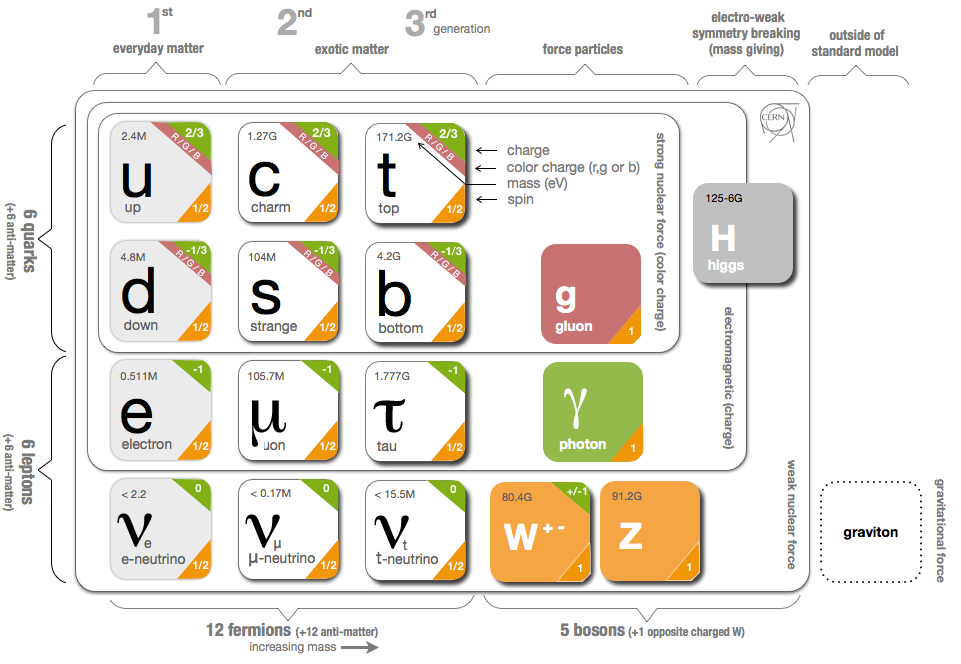
\includegraphics[width=12cm]{SM_chapter_plots/SM}
\label{SMfigure}\caption{Particles of the Standard Model}
\end{figure}

\subsection{Electroweak Interaction}

The SM propose a doublet representation for the left-handed fields and singlets for the right-handed fields:
\begin{eqnarray}
L^{i}=\left(
\begin{array}{c}
\displaystyle \nu_{e L}\\
\displaystyle e_{L}
\end{array}\right),
\left(
\begin{array}{c}
\displaystyle \nu_{\mu L}\\
\displaystyle \mu_{L}
\end{array}\right),
\left(
\begin{array}{c}
\displaystyle \nu_{\tau L}\\
\displaystyle \tau_{L}
\end{array}\right),
\qquad
Q^{i}=\left(
\begin{array}{c}
\displaystyle u_{L}\\
\displaystyle d_{L}
\end{array}\right),
\left(
\begin{array}{c}
\displaystyle c_{L}\\
\displaystyle s_{L}
\end{array}\right),
\left(
\begin{array}{c}
\displaystyle t_{L}\\
\displaystyle b_{L}
\end{array}\right).        
\end{eqnarray}
\begin{eqnarray}
e_{R}^{i} &=& \left\lbrace e_{R}, \mu_{R}, \tau_{R} \right\rbrace ,  \nonumber\\
u_{R}^{i} &=& \left\lbrace u_{R}, c_{R}, t_{R} \right\rbrace , \qquad d_{R}^{i} = \left\lbrace d_{R}, s_{R}, b_{R} \right\rbrace .
\end{eqnarray}
Where $i$ runs over the generations of fermions. The $L$ (left-handed) and $R$ (right-handed) indices appears because the projections operators were applied over the wave functions, where $\psi_{L}=P_{L}\psi$ and $\psi_{R}=P_{R}\psi$, with $P_{L}=(1-\gamma^{5})/2$ and $P_{R}=(1+\gamma^{5})/2$.\\
The free massless fermionic lagrangian is:
\begin{displaymath} 
\lagrangean_{f}=\frac{i}{2}\sum^{3}_{i=1}\left\{\:\bar{L}^{i}\:\not\! \partial\:L^{i}+\:  \bar{Q}^{i}\:\not\! \partial\:Q^{i}+\:\bar{e}_{R}^{i}\:\not\! \partial\:e_{R}^{i} + \:\bar{u}_{R}^{i}\:\not\! \partial\:u_{R}^{i} + \:\bar{d}_{R}^{i}\:\not\! \partial\:d_{R}^{i}  \right\}+\hbox{h.c}
\end{displaymath}
with $\bar{\psi}=\psi^{\dag}\:\gamma^{0}$.\\
The proposed Lagrangian must be invariant under local gauge transformations:
\begin{eqnarray}
\Psi_{i}\:'&=&\:\hbox{exp}\left[i\:\alpha(x)_{j}\sigma_{j}+i\:\beta(x)Y\right]\Psi_{i}\nonumber\\
\chi_{i}\:'&=&\:\hbox{exp}\left[i\:\beta(x)Y\right]\:\chi_{i}  
\end{eqnarray}
where $\Psi_{i}=\left\{L^{i},Q^{i}\right\}$ and $\chi_{i}=\left\{e_{R}^{i}, u_{R}^{i}, d_{R}^{i} \right\}$. Also, 
 $\alpha$ and $\beta$ are parameters belonging to the symmetry groups $SU(2)$ and $U(1)$ respectively, $\sigma_{j}$ are the Pauli matrices and $Y$ is the hypercharge.
In order to mantain the gauge invariance after the transformations, we have to introduce the covariant derivatives:
\begin{eqnarray}
D_{L}^{\:\mu}&=&\;\partial^{\mu}-\:i\:\left(g/2\right)\:\sigma_{j}\:A^{\mu}_{j}+\:ig'\:B^{\:\mu}\:Y\;\nonumber\\
D_{R}^{\:\mu}\:&=&\;\partial^{\mu}+\:i\:g'\:B^{\:\mu}\:Y\;\:
\end{eqnarray}
Finally we get:
\begin{eqnarray}\label{leptonico}
\lagrangean_{f}=\frac{i}{2}\sum^{3}_{i=1}\left\{\:\bar{L}^{i}\:\not\!\! D_{L}\:L^{i}+\:\bar{Q}^{i}\:\not\!\! D_{L}\:Q^{i}+\:  \bar{e}_{R}^{i}\:\not\!\! D_{R}\:e_{R}^{i}+\:  \bar{u}_{R}^{i}\:\not\!\! D_{R}\:u_{R}^{i}+\:  \bar{d}_{R}^{i}\:\not\!\! D_{R}\:d_{R}^{i}\right\}+\hbox{h.c}\nonumber\\
\end{eqnarray}
where $\not\!\! D\equiv \displaystyle\gamma_{\mu}D^{\:\mu}$ and $g'$, $g$ are the coupling constants of the groups $U(1)$ and $SU(2)$ respectively. $A^{\mu}$, $B^{\mu}$ are gauge fields.\\
\indent
So far we have presented the Lagrangian of fermions and their interactions with the gauge fields via the covariant derivative. The complete Lagrangian density of SM should also contain terms that describe the gauge bosons when there is no fermions involve (free bosonic Lagrangian).
These expressions should also be locally gauge invariants under $SU(2)_{L}\otimes U(1)_{Y}$. Similarly in the case of fermions we assume, for the moment,  massless gauge bosons. The bosonic lagrangian is:
\begin{eqnarray}\label{bosott}
\lagrangean_{B}=\frac{1}{2g^{2}}\:\hbox{Tr} \left(\mathcal{F}_{\mu\nu}\:\mathcal{F}^{\mu\nu}\right)-\frac{1}{4}B_{\mu\nu}\:B^{\mu\nu}
\end{eqnarray}
\begin{flushleft}
where the fields are expressed as function of the group generators
\begin{eqnarray*}
\mathcal{ F}_{\mu\nu}(x)=-\frac{ig}{2}\sigma_{a}F^{a}_{\mu\nu}(x),\ \ \ \ \  A_{\mu}(x)=-\frac{ig}{2}\sigma_{a}A^{a}_{\mu}(x)
\end{eqnarray*}
resulting:
\begin{eqnarray}
\lagrangean_{B}&=&-\frac{1}{4}\sum^{3}_{a=1}F^{a}_{\mu\nu}F^{\mu\nu a}-\frac{1}{4}B_{\mu\nu}B^{\mu\nu}
\end{eqnarray}
To maintain the local gauge invariance of the Lagrangian, it follows that:
\end{flushleft}
\begin{eqnarray}
F^{a}_{\mu\nu}&=&\partial_{\mu}A^{a}_{\nu}-\partial_{\nu}A^{a}_{\mu}+g\:\epsilon^{a}_{bc}\:A^{b}_{\mu} A^{c}_{\nu},\ \ \ \ \ \ \ \ \ a=\hbox{1,2,3.}\nonumber\\
B_{\mu\nu}&=&\partial_{\mu}B_{\nu}-\partial_{\nu}B_{\mu}
\end{eqnarray}
The Lagrangian (\ref{bosott}) involves gauge fields connected with the groups $SU(2)_{L}$ and $U(1)_{Y}$ and, the number of fields is related to the number of group generators. In our case we have four gauge fields $A^{1}$, $A^{2}$, $A^{3}$ and $B$.\\

\subsection{Strong Interaction}

The Strong interaction between quarks and gluons in the SM, is described by the Quantum Chromodynamics (QCD). The QCD is a non-abelian gauge field theory based on the  symmetry group $SU(3)_{C}$.
The Lagrangian of QCD, invariant under $SU(3)_{C}$ gauge transformations, is given by:
\begin{eqnarray}
\lagrangean_{S}&=&\sum_{q}\:\bar{\psi}_{q,a}\left( i\not\!\! D -m_{q} \right)\psi_{q,a} - \dfrac{1}{4}\:G^{A}_{\mu\nu}G^{A \mu\nu} 
\end{eqnarray}
The $\psi_{q,a}$ are quark-field spinors for a quark flavor $q$ and mass $m_{q}$, with a color index $a$ that runs from $a=1$ to $N_{C}=3$. In order to maintain gauge invariant, the covariant derivative take the form:
\begin{eqnarray}
D_{\mu} = \partial_{\mu} + ig_{S}\dfrac{\lambda_{A}}{2}\mathcal{A}_{\mu}^{A} 
\end{eqnarray}  
where $g_{S}$ is the QCD coupling constant, $\lambda_{A}$ the Gell-Mann matrices and $\mathcal{A}_{\mu}^{A}$ the gauge field of the gluons where $A$ runs from $A=1,\dots,8$. The field tensor $G^{A}_{\mu\nu}$ is given by:
\begin{eqnarray}\label{gluon}
G^{A}_{\mu\nu}&=&\partial_{\mu}\mathcal{A}^{A}_{\nu}-\partial_{\nu}\mathcal{A}^{A}_{\mu}+g_{S}\:f_{ABC}\:\mathcal{A}^{B}_{\mu} \mathcal{A}^{C}_{\nu},\ \ \ \ \ \
\left[ \lambda_{A}, \lambda_{B} \right] = 2if_{ABC}\lambda_{C}
\end{eqnarray}
where $f_{ABC}$ are the structure constants of the $SU(3)$ group.

\subsection{Spontaneous Symmetry Breaking}\label{QES}

Until now all the fermions and gauge bosons were considered massless, but in reality for all particles proposed in the SM only
the photons are massless. The simple addition of the mass terms to the Lagrangian density spoils the gauge invariance and the renormalization of the theory.\\
\indent
In order to maintain the theory renormalizable it is essential to introduce the masses by a mechanism that keeps the gauge invariance
of the Lagrangian density, this is achieved through the Higgs mechanism \cite{Higgs:1966ev}.\\
\indent
This mechanism uses the spontaneous symmetry breaking  (SSB), initially proposed by  by Goldstone, Salam and Weinberg \cite{PhysRev.127.965}, which states that under a certain symmetry transformation, the Lagrangian remains invariant, but not so the vacuum state. If the symmetry is global, a massless particle appears which is called the Nambu-Goldstone boson \cite{PhysRevLett.4.380,Goldstone:1961eq}.\\
\indent
When this method is applied in a local gauge theory, something amazing happens: the Nambu-Goldstone bosons are absorbed by gauge particles and turn massless particles on massive ones. This is called Higgs-Kibble mechanism \cite{Higgs:1966ev,PhysRev.155.1554}.
Now we construct a local gauge invariant Lagrangian for
zero spin particles, consisting of a free or kinetic part and a potential. By introducing the covariant derivative in the kinetic term, we ensure their gauge invariance.
Then we have:
\begin{eqnarray}
\lagrangean_{H}=\left[D^{\mu}\Phi\right]^{\dagger}\left[D_{\mu}\Phi\right]+\mu^{2}\Phi^{\dagger}\Phi-\lambda^{2}\left[\Phi^{\dagger}\Phi\right]^{2}
\end{eqnarray}
where $\Phi$ is a scalar complex field  which transform as a $SU(2)_{L}$ doublet :
\begin{eqnarray}
\Phi=\left(\begin{array}{c}
\phi^{+}\\
\phi^{0}
\end{array}\right)
\end{eqnarray}
To meet gauge invariance: 
\begin{eqnarray}
D_{\mu}\:=\left[\;\partial_{\mu}-\:\frac{i\:g}{2}\:\sigma_{j}\:A^{j}_{\mu}+\:\frac{ig'}{2}Y\:B_{\mu}\;\right]\:\nonumber
\end{eqnarray}
In a similar way, $g$ y $g'$ are the coupling constants, $\sigma_{j}$ and $Y$ are the generators, and $B_{u}$ and $A^{j}_{\mu}$ are the gauge fields of the groups $U(1)_{Y}$ and $SU(2)_{L}$ respectively.\\
The SSB implies that the Higgs field expand over the vacuum.
\begin{eqnarray}
\Phi=\frac{1}{\sqrt{2}}\left(\begin{array}{c}
0\\
v+h(x)
\end{array}\right)
\end{eqnarray}
where $v$  is the vacuum expectation value and $h$ is the Higgs field.

\subsection{Yukawa Lagrangian}

In the previous section the Higgs field was introduced in order to generate mass for the SM particles. The gauge bosons couples with the scalar field through the covariant derivative, but in the case of fermions, they not show 
any link with the scalar field. For that reason, we need to
introduce a new Lagrangian (by hand) in which the Higgs field engages with the fermions: 
\begin{equation}\label{yukawa}
\lagrangean_{Y}=-\sum_{\lepton=1}^{3} G_{\lepton}\left[\bar{L}^{\lepton}\Phi\:e^{\lepton}_{R}\:\right]- \sum_{i,j=1}^{3}\left[\:\Gamma^{u}_{ij}\:\bar{Q}^{i}\:\tilde{\Phi}\:u^{j}_{R} + \Gamma^{d}_{ij}\:\bar{Q}^{i}\:\Phi\: d^{j}_{R}  \right]  
+\hbox{h.c.} 
\end{equation}
with
\begin{equation}
\tilde{\Phi} \equiv i\tau^{2}\Phi^{\dag}=\left(\begin{array}{c}
\phi^{0 \dag}\\
-\phi^{-}
\end{array}\right) 
\end{equation}
where the index runs over the number of generations, and the $\Gamma^{u},\Gamma^{d}$ are 3x3 matrices which determine the fermion masses and mixings.
This lagrangian is know as Yukawa Lagrangian.\\
After the SSB we obtain the complete Lagrangian density of the SM, in the unitary gauge:
\begin{eqnarray}
\lagrangean &=& \bar{\psi}_{f}\left(i \:\not\! \partial-m_{f} \right)\psi_{f}\nonumber\\
&-&\dfrac{1}{4}F_{\mu\nu}F^{\mu\nu}-\dfrac{1}{4}G^{A}_{\mu\nu}G^{A \mu\nu}\nonumber\\
&-&\dfrac{1}{2}F^{\dag}_{W \mu\nu}F^{\mu\nu}_{W} + m_{W}^{2}W^{\dag}_{\mu}W^{\mu}\nonumber\\
&-&\dfrac{1}{2}Z_{\mu\nu}Z^{\mu\nu} +\dfrac{1}{2}m_{Z}^{2}Z_{\mu}Z^{\mu}\nonumber\\
&+& \dfrac{1}{2} \left(\partial_{\mu} h \right)\left(\partial^{\mu} h \right)- \dfrac{1}{2} m_{H}^{2}h^{2} + \text{interaction terms}   
\end{eqnarray}
where :
\begin{eqnarray}
F^{\mu\nu} &=& \partial^{\nu}A^{\mu}-\partial^{\mu}A^{\nu} \nonumber\\
F^{\mu\nu}_{W} &=& \partial^{\nu}W^{\mu}-\partial^{\mu}W^{\nu} \nonumber\\
Z^{\mu\nu} &=& \partial^{\nu}Z^{\mu}-\partial^{\mu}Z^{\nu}
\end{eqnarray}
are the fields related with the photon, W boson and Z boson respectively. The field $\psi_{f}$ runs over all the fermions and   $G^{A}_{\mu\nu}$ is the gluon field previously defined in (\ref{gluon}). The mass terms are given by:
\begin{eqnarray}
m_{\lepton} &=& \dfrac{G_{\lepton} v}{\sqrt{2}}\\
m_{W} &=& \dfrac{1}{2} vg\\
m_{Z} &=& \dfrac{1}{2} v\sqrt{g^{2}+g'^{2}}\\
m_{H} &=& \sqrt{ 2 v^{2} \lambda}
\end{eqnarray}



\section{Beyond Standard Model}

Although the Standard Model accurately describes the fundamental interations in nature and agrees with all the experimental data we have at our disposal today it is still incomplete. Perhaps it is only a part of a bigger picture that includes new physics. Some of the unanswered main questions are:  Why is the weak scale so much smaller than the Planck scale?  What is the origin of the difference between matter and antimatter, and is it related to the origin of the matter in the Universe? What is the nature of the astrophysical dark matter? How does one unify the fundamental interactions?\\
\indent
In this section we will give a little insight into some of these problems and some models which try to give an answer.

\subsection{The Hierarchy Problem}\label{hierarchy}

When radiative corrections are performed to the Higgs mass, for example at one loop level (\cref{figurehiggsmass}), one needs to integrate over  the momentum of the virtual particles. In general we have to limit the integral by a cut-off ($\Lambda$) related with  the next energy scale in the theory.
If the next scale is gravity, $\Lambda$ is the Planck scale $M_{P} \sim 10^{18}$ \gev. Thus, if the SM were valid up to the Planck scale, then the Higgs mass $m_{H}$,	and therefore the minimum of the Higgs potential $v$ , would be driven from the weak scale to the Planck scale by the radiative corrections (eqn. \ref{higgsmasseq}).
\begin{figure}[H]
  \centering
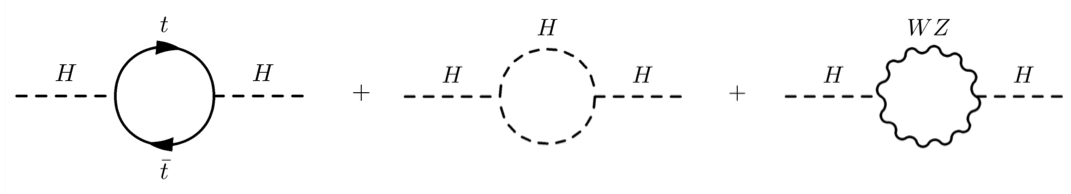
\includegraphics[width=15cm]{SM_chapter_plots/higgsmass}
\caption{Radiative Corrections to the Higgs Mass. \label{figurehiggsmass}}
\end{figure}
\begin{eqnarray}\label{higgsmasseq}
m_{H}^{2} = m_{H,0}^{2} + \dfrac{3 g^{2}}{32 \pi^{2}}\dfrac{\Lambda^{2}}{m_{W}^{2}}\left[ m_{H}^{2} + 2m_{W}^{2} + m_{Z}^{2} - \dfrac{4}{3} m_{t}^{2}  \right] 
\end{eqnarray}
To avoid this, one
has to adjust the Higgs bare mass $m_{H,0}$ to one
part in $10^{17}$. This is quite unnatural, and is what we call the
gauge \textbf{hierarchy problem}.
In order to solve this unnatural fine tunning some theories beyond SM were proposed, for example, Supersymmetry (SUSY), Composite Higgs and Extra Dimensions. We will focus only in the last of these models.

\subsection{Dark Matter}

Dark matter is a hypothetical kind of matter that cannot be seen with telescopes but accounts for most of the matter in the universe. Dark matter neither emits nor absorbs light or any other electromagnetic radiation at any significant level. This means that it has not electric charge and can interact only via gravitational force, or weak force similar to neutrinos.
The existence and properties of dark matter are inferred from many sources,
\paragraph{Velocity curves of spinning galaxies} In 1970 an American astronomer, Vera Rubin, measured the speed of stars in rotating galaxies accurately enough to convince the scientific community. She observed that stars in spinning galaxies were all rotating at roughly the same velocity, no matter their distance to the galactic centre. This is in contradiction with Kepler’s law that describes the rotation of planets around the Sun.  This could only happen if huge amounts of invisible matter filled the entire galaxy and beyond.
\paragraph{Gravitational lensing} We know that light moves in a straight line in free space. In the presence of a massive object such as a star or a galaxy, the space is deformed and light follows the curvature of the distorted space. Light coming from a distant galaxy will bend when passing near a massive clump of dark matter and the galaxy will appear shifted, as if coming from different places.
\paragraph{Cosmic microwave background} Astrophysicists can infer how much dark matter exists by studying the cosmic microwave background. From the amount of radiation associated to each frequency, astrophysicists can calculate the quantity of dark matter contained in the Universe.\\

\indent Experiments at the (LHC) may supply more direct evidence about dark matter. According to many theories, dark matter particles would be light enough to be produced at the LHC. If they were generated at the LHC, they would escape through the detectors leaving no signal. However, they would transport energy and momentum, so one could infer their existence from the amount of energy and momentum "missing" after a collision. Dark matter candidates arise frequently in theories that suggest physics beyond the Standard Model, such as Supersymmetry and Extra Dimensions.

\subsection{Extra Dimensions}

Why is gravity so much weaker than the other fundamental forces?  One possibility is that we don’t feel the full effect of gravity  because part of it spreads to extra dimensions. If extra dimensions exist, they could explain why gravity is weaker than the other forces of nature.

How could we test for extra dimensions? 
Some theorists suggest that a particle called the "graviton" is associated with gravity. If gravitons exist, it should be possible to create them at the LHC, but they would rapidly disappear into extra dimensions. A graviton might escape our detectors, leaving an empty zone that we notice as an imbalance in momentum and energy in the event. We would need to carefully study the properties of the missing object to work out whether it is a graviton escaping to another dimension or something else. This method of searching for missing energy in events is also used to look for dark matter or supersymmetric particles.

	

\subsubsection{Large Extra Dimensions}

The reason why we have not observed the extra dimensions yet is that contrary to the ordinary four space-time dimensions which are very large (or infinite), these hypothetical extra dimensions are finite, that is they are compactified. The  question that one needs to ask is how large could the size of the extra dimensions be without getting into conflict with observations.\\
\indent 
Assuming that there are $n$ extra dimensions, calling the fundamental Planck scale of the theory (in $4+n$ dimension) $M_{*}$, the usual Planck scale (in 4 dimensions) $M_{Pl}$, $r$ the compactification radius of the extra dimension, and using the matching for the gravitational and the gauge coupling, it is found that \cite{Csaki:2004ay}:
\begin{eqnarray}
M_{Pl}^{2} &=& M_{*}^{n+2}V_{(n)}= M_{*}^{n+2}\left(2 \pi r \right)^{n} \sim r^{n}M_{*}^{n+2}\label{planck}\\ 
\dfrac{1}{g_{4}^{2}} &=& V_{(n)}M_{*}^{n} \sim r^{n}M_{*}^{n}
\end{eqnarray}
In the second equation we assume that the gauge field propagates in all dimensions. Considering that the spacetime is flat, and that the $n$ extra dimensions are compact, where $V_{n}$ is the volume of the extra dimensional space and $g_{4}$ is the coupling constant. From these two equations it is obtainned:
\begin{eqnarray}
r \sim \dfrac{1}{M_{Pl}}\:g_{4}^{\frac{n+2}{n}}
\end{eqnarray}
This would imply that in a higher dimensional theory $r \sim 1/M_{Pl}$. In this case there would be no hope of finding these tiny extra dimensions. Now, we will investigate what happen if, instead of the previous assumption, the SM fields were localized in 4 dimensions, and only gravity were to propagate into the extra dimension. 
In that case new phenomena will appear in the gravitational sector when you reach distances as short as the size of the extra dimension. However, it is very hard to test gravity at very short distances. The bound in the size of the extra dimension ($r\leq$ \unit[0.1]{mm}) is given by Cavendish type experiments if only gravity propagates in the extra dimension.\\ 
\indent
For $M_{*}\sim$ \unit[1]{TeV} the model is called "Large Extra Dimensions", proposed by Arkani-Hamed, Dimopoulos and Dvali (ADD) \cite{ArkaniHamed:1998rs}.
From (eqn. \ref{planck}) we find:
\begin{eqnarray}
r \sim 2\times 10^{17}\times 10^{\frac{32}{n}} \text{cm}
\end{eqnarray}
Therefore, if we select $n=1$ , we get that $r\sim 10^{8}$ Km, which is certainly excluded. Taking $n=2$ , one has $r \sim 1$ mm, which is a distance scale already constrained by Cavendish-type experiments.\\
\indent
The fact that gravity propagates in compact extra dimensions leads to the existence of graviton excitations with a mass gap given by $\Delta m \sim 1/R$.
The graviton in this $(4+n)$-dimensional formulation can be equivalently expressed as a set of 3-dimensional Kaluza–Klein (KK) modes  with different graviton masses. The coupling of the KK modes to the SM energy–momentum tensor leads to an effective theory with virtual-graviton exchange at leading order (LO) in perturbation theory. An ultraviolet (UV) cutoff must be introduced to avoid divergences in the summed contributions from all modes.


\subsubsection{Universal Extra Dimensions}

Universal Extra Dimensions \cite{PhysRevD.64.035002} are models in which all of the SM fields live in $4+n$ dimensions with the $n$ extra dimensions taken to be flat and compact. 
In the Minimal Universal Extra Dimensions (MUED) we have five dimensions, namely only one extra dimension. In this model the hierarchy problem is not addressed but have some interesting features as a stable dark matter candidate.
In this case the extra dimension is compactified in a circle of radius $r$. 
The key element is the conservation of momentum in the universal dimensions. In the equivalent four-dimensional theory this implies KK number conservation. For example, in five dimensions (5D), $p_{5}$ the fifth component of the 5D momentum is quantified and given by
\begin{eqnarray}
p_{5} = n/r
\end{eqnarray}
Promoting the full SM to extra dimensions bring some problems, for example the fermions are generically non-chiral (with respect to our four dimensions). This problem is solved by "orbifolding", \ie, compactifying on surfaces with endpoints. In five dimensions, the only choice is $S^{1}/Z_{2}$, which identifies opposite sides of a circle to create a line segment with two endpoints.

\begin{figure}[H]
  \centering
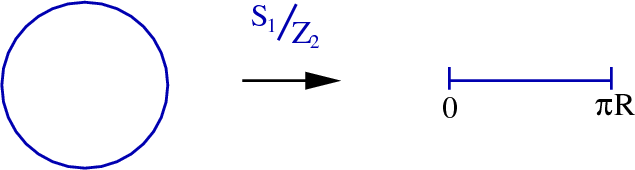
\includegraphics[width=12cm]{SM_chapter_plots/orbifold}
\label{orbifigure}\caption{orbifold}
\end{figure}

As a consequence of the orbifolding, translational invariance along the 5th dimension is broken, which results that the KK-number conservation is broken too, but there is a remnant left: the parity
of the KK modes must be conserved at	 the vertex. In addition, KK-parity conservation means that the lightest state of
the first KK level cannot decay into zero-modes, making it
stable and a candidate for dark matter.
The masses of the KK modes at tree levl are given by:
\begin{eqnarray}
m_{n}^{2} = \dfrac{n^{2}}{r^{2}}+ m_{SM}^{2}
\end{eqnarray}
with $n=0,1,2,\dots$. Note that for $n=0$ (zero mode) we obtain the mass on the SM particles. In general the mass of the SM particles are smaller than the compactification radius of the extra dimension, so the KK modes are practically degenerate. Radiative corrections generate mass splittings, but these are still
small enough for the energy yield to be small in the production and subsequent decay of KK states.

\subsubsection{Warped Extra Dimension}

\paragraph{Randall Sundrum (RS) Models}

Lisa Randall and Raman Sundrum proposed a model where there is only one warped extra dimension which is compactified on the $S^{1}/Z_{2}$ orbifold \cite{Randall:1999ee,Randall:1999vf}. Two 4D branes (the Planck brane and the TeV brane) are separated by the fifth extra dimension with size $r_{c}$ (fig. \ref{RSfigure}). Even though the extra dimension is curved, the brane itself remains static and flat, that is, it preserves 4D Lorentz invariance. This means that the induced metric at every point along the extra dimension has to be the ordinary flat 4D Minkowski metric, and the components of the 5D metric depend only on the fifth coordinate $y$. The ansatz for the most general metric satisfying these properties is given by:
\begin{eqnarray}
ds^{2}= e^{-A(y)} dx^{\mu}dx^{\nu} \eta_{\mu\nu} - dy^{2} 
\end{eqnarray}
Where $\eta_{\mu\nu}=\text{diag}(-1,1,1,1)$ and the amount of curvature (warping) along the extra dimension depends on the function $e^{-A(y)}$, which is therefore called the warp-factor. This
type of geometry is called "non-factorizable" because the metric of the 4D subspace is $y$-dependent.
In the simplest version of the RS model it is assumed that the SM fields live on the so-called TeV brane while gravity lives everywhere. Unlike the ADD case, however, there is a "cosmological" constant in the 5D bulk and both branes have distinct tensions. Solving the 5D Einstein’s equations provides a unique solution for these quantities and also determines that $A(y) = k\left| y \right| $, where k is a dimensionful parameter. A basic assumption of this model is that there are no large mass hierarchies present, so that we expect that $k \sim M_{*}$, the 5D fundamental or Planck scale. In fact, once we solve Einstein’s equations and plug the solutions back into the original action and integrate over $y$ we find that:
\begin{eqnarray}
M_{Pl}^{2} = \dfrac{M_{*}^{3}}{k}\left(1-e^{-2\pi k r_{c}} \right)  
\end{eqnarray}
The warp factor $e^{-\pi k r_{c}}$ will be a very small quantity which implies that $M_{Pl}$, $M_{*}$ and $k$ have essentially comparable magnitudes following from the assumption that no hierarchies exist. If we calculate the Ricci
curvature invariant for this 5D space, we find that it is  constant, $ R_{5} = - 20 k^{2}$ and thus $k$ is a measure of the
constant curvature of this space. A space with constant negative curvature is called an Anti-DeSitter space and so this 5D version is called $AdS_{5}$.
\begin{figure}[H]
  \centering
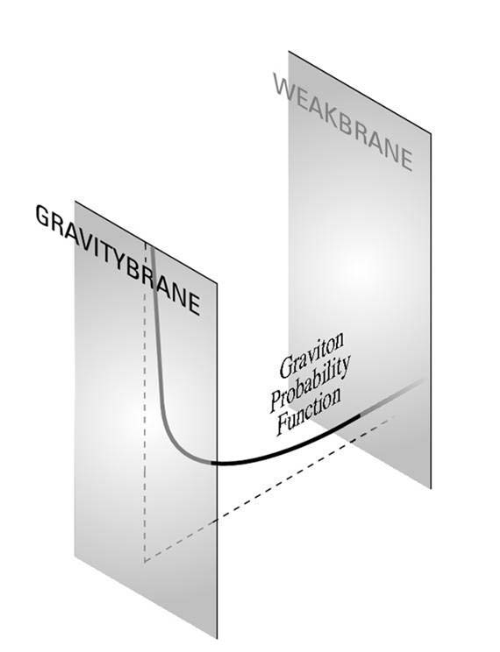
\includegraphics[width=6cm]{SM_chapter_plots/RS}
\caption{Graviton probability function \label{RSfigure}}
\end{figure}

It will be assumed that all dimensionful parameters in the action will have their mass scale set by $M_{*} \sim M_{Pl} \sim k$ so that there is no fine-tuning. However, the warp factor rescales them as one moves about in $y$ so that, in particular, all masses will appear to be of order the
TeV scale on the SM brane. This means that if there is some mass parameter, $m$, in the action which is order $M_{Pl}$, we on TeV brane will measure it to be reduced by the warp factor, i.e., $me^{-\pi k r_{c}}$. Note that if $kr_{c} \sim 11$ (a
small hierarchy) this exponential suppression reduces a mass of order $10^{18}$ GeV to only 1 TeV. Thus the ratio of the weak scale to $M_{Pl}$ is explained through an exponential factor and no large ratios appear anywhere else in the model. It has been shown by Goldberger and Wise \cite{Goldberger:1999un} that values of $kr_{c} \sim 11$ are indeed natural and can be provided by a stable configuration. Hence we have obtained a true solution to the hierarchy problem.
If we consider the action for the Higgs field on the TeV brane:
\begin{eqnarray}
S = \int d^{4}x dy \sqrt{-g} \left(g^{\mu\nu}\partial_{\mu}H^{\dag}\partial_{\nu}H-\left(H^{2}-v_{0}^{2} \right)^{2}\right)\delta\left(y-\pi r_{c} \right)     
\end{eqnarray}
From this we see that the vev that we observe on the SM brane is not $v_{0}$ but
\begin{eqnarray}
v = v_{0} e^{ -\pi k r_{c}}
\end{eqnarray}
which is of order the TeV scale.
Even though gravitons are spin-2, it turns out that their masses
and wave functions are identical to the case of a scalar field in the RS bulk which is far simpler to analyze. If we solve the Klein-Gordon equation, but now in the case of curved space, after a separation of variables via the KK decomposition the solutions are linear combination of $J_{2}$, $Y_{2}$ Bessel functions and the mass of the KK states are given by: 
\begin{eqnarray}
m_{n} = x_{n} k e ^{-\pi r_{c}}
\end{eqnarray}
where $x_{n}$ are roots of $J_{1}(x_{n})=0$. Here $x_{n} = 0, 3.8317, 7.0155, 10.173, \dots$ etc. Since $k e^{-\pi k r_{c}}$ is of the order of a few hundred GeV at most, we see that the KK graviton masses are of similar magnitude with comparable, but unequal, spacing, i.e., the KK gravitons have approximately weak/TeV scale masses. We thus have weak scale graviton KKs with weak scale couplings that should be produced as spin-2 resonances at colliders.

\paragraph{Bulk Graviton Model}

Different models with warped extra dimensions allow the SM fields to propagate in the ED. In these models, as a consequence of the localization of SM particles near the Planck or the TeV brane, decays to diphotons and dileptons are suppressed by a factor proportional to the volume of the extra dimension. This scenario is more compatible with electroweak precision tests and limits on flavor-changing neutral current processes than the original RS1. The different couplings of the graviton to the SM fields result in two distinctive effects: the branching fraction to SM vector-boson pairs can become dominant for certain values of the model parameters, and a very strong enhancement in the longitudinal polarization of the vector bosons is predicted. Because of the aforementioned suppression of photon and fermion couplings, the total production cross section is also smaller with respect to RS1 gravitons: in the Agashe–Davoudiasl–Perez–Soni (ADPS) model \cite{Agashe:2007zd} for $M = 700$ GeV and $\tilde{k}= 0.50$ , it amounts to 0.31 pb in pp collisions at $\sqrt{s} = 7$ TeV, and the branching fraction to longitudinally polarized ZZ bosons is about 12$\%$.






\chapter{CMS Experiment}

\section{Large Hadron Collider (LHC)}

The Large Hadron Collider is the largest and most powerful particle accelerator ever built. It boost protons, to produce two beams travelling in opposite directions, which collide at four points where the two rings of the machine intersect.\\
\indent
The design energy per proton beam is of 7 TeV. The protons of the LHC circulate around the ring in well defined
bunches. In the LHC, under nominal operating conditions, each proton beam has 2808 bunches, with each bunch containing about 10$^{11}$ protons. They measure a few centimetres long and a millimetre wide when they are far from a collision point. As they approach the
collision points, they are squeezed to about 16 $\mu$m to allow for a greater chance of proton-proton collisions. The LHC uses a bunch spacing of 25 ns (or about 7 m), which  corresponds to a frequency of 40 MHz \cite{lhc}. Nowdays, each proton beam flying around the LHC have an energy of 6.5 TeV, so when two protons collide the collision energy is 13 TeV.\\
\indent
There are seven experiments installed at the LHC (Fig. \ref{fig:LHC}); The biggest experiments consist in two general-purpose detectors to investigate the largest range of physics possible : The Compact Muon Solenoid (CMS) and A Toroidal LHC ApparatuS (ATLAS), and two specialized for focussing on specific phenomena: A Large Ion Collider Experiment (ALICE) and Large Hadron Collider beauty experiment(LHCb).
The smaller experiments on the LHC are the TOTal Elastic and diffractive cross section Measurement (TOTEM), Large Hadron
Collider forward experiment (LHCf) and the Monopole and Exotics Detector at the LHC (MOEDAL). The first two experiments are  focused on "forward particles", protons or heavy ions that brush past each other rather than meeting head on when the beams collide and the last experiment searches for a hypothetical particle called the magnetic monopole.  
TOTEM will be installed close to the CMS interaction point, LHCf will be installed near ATLAS and MOEDAL near LHCb. 

\begin{figure}[H]
  \centering
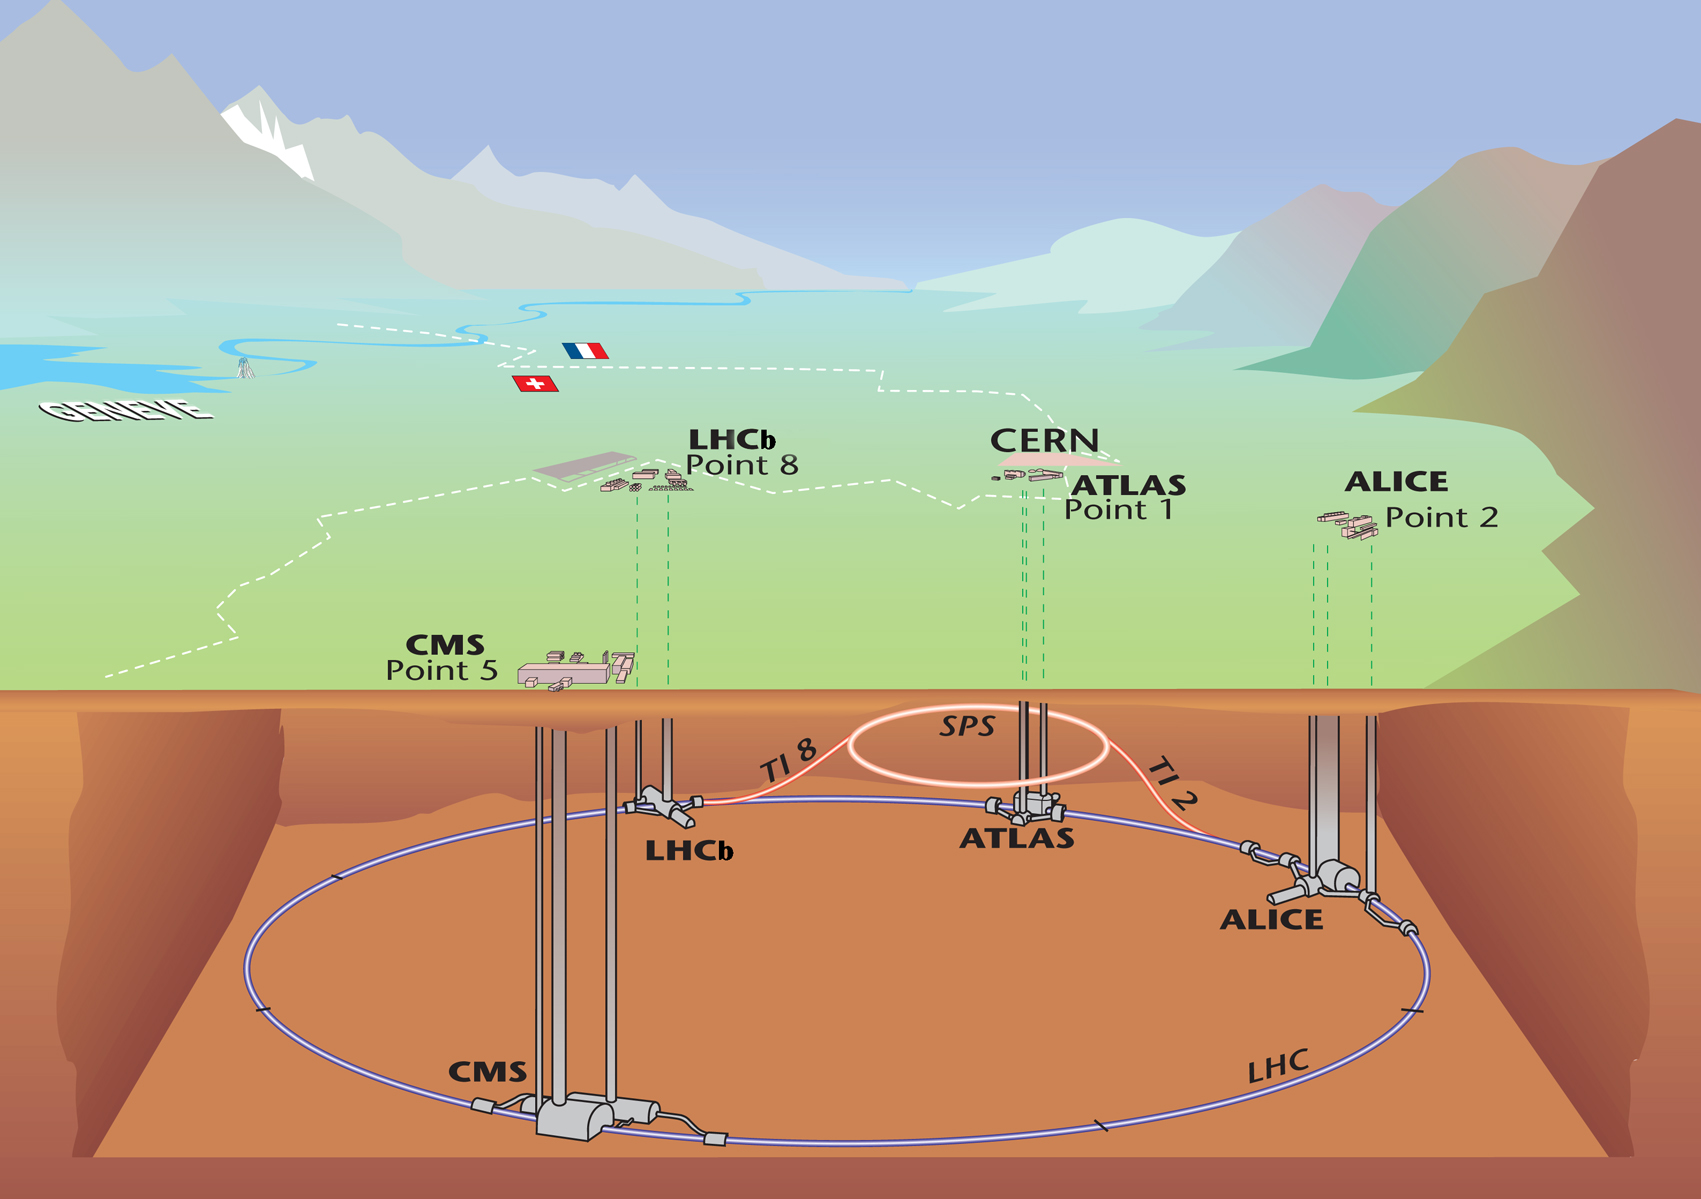
\includegraphics[width=10cm]{CMS_chapter_plots/lhc}
  \caption{Overall view of the LHC experiments \label{fig:LHC}}
\end{figure}
\noindent


\section{CMS Detector}

The central feature of the CMS apparatus is a superconducting solenoid of \unit[6]{m} internal diameter, providing a magnetic field of \unit[3.8]{T}.\\
\indent
Within the superconducting solenoid volume are a silicon pixel and strip tracker, a lead tungstate crystal electromagnetic calorimeter (ECAL), and a brass and scintillator hadron calorimeter (HCAL), each composed of a barrel and two endcap sections. Muons are measured in gas-ionization detectors embedded in the steel flux-return yoke outside the solenoid. Extensive forward calorimetry complements the coverage provided by the barrel and endcap detectors.\\

\begin{figure}[H]
  \centering
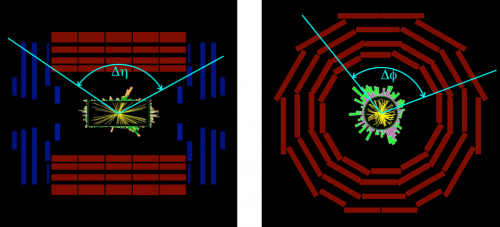
\includegraphics[width=12cm]{CMS_chapter_plots/image_eta}
\label{eta}\caption{$\eta$ and $\phi$ coordinates in the CMS detector}
\end{figure}
\noindent
\indent
A right-handed coordinate system is used with its origin at the nominal interaction point (IP). The x-axis points to the center of
the LHC ring, the y-axis is vertical and points upward, and the z-axis is parallel to the counterclock-wise beam direction. The azimuthal angle $\phi$ is measured with respect to the x-axis in the xy-plane and the polar angle $\theta$ is defined with respect to the z-axis, while the pseudorapidity is defined as $\eta = -\ln\left[\tan\left(\theta/2 \right)  \right]$. 

\begin{figure}[h]
  \centering
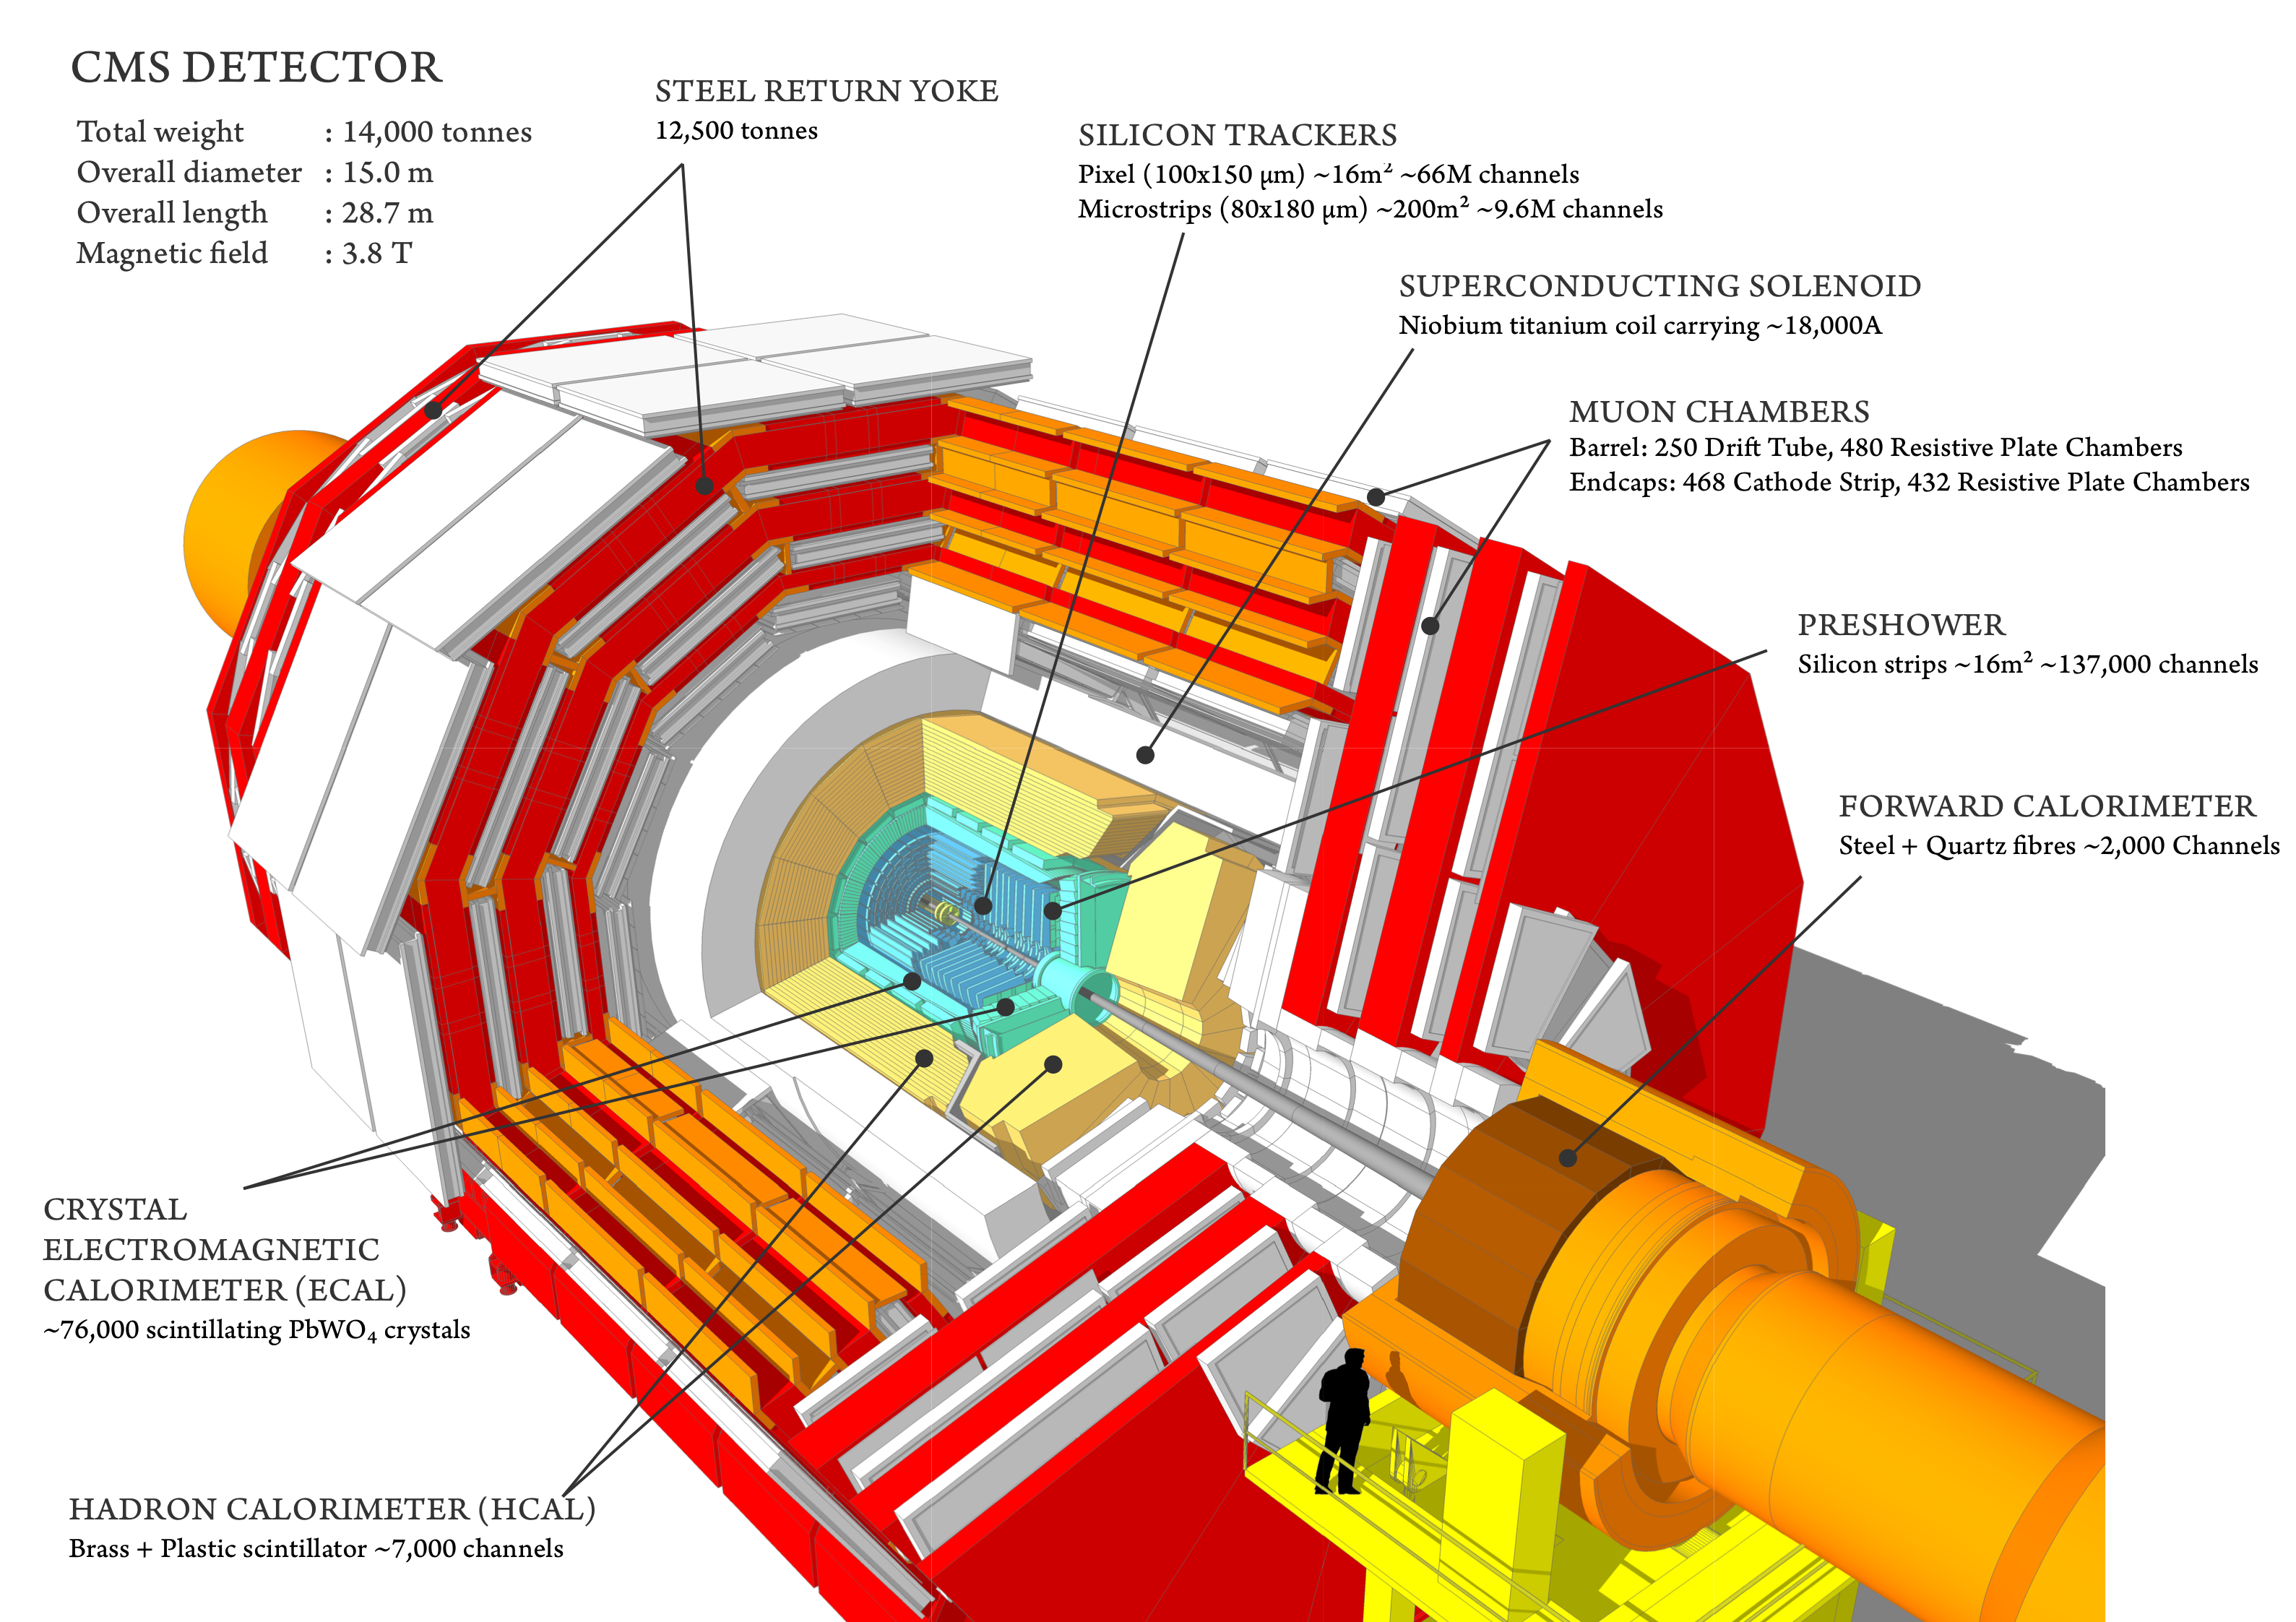
\includegraphics[width=15cm]{CMS_chapter_plots/cms_120918_03}
\label{figure}\caption{Schematic view of the CMS detector}
\end{figure}


\subsection{CMS sub-detectors and components}

\subsubsection{The Magnet}

The CMS collaboration has decided to operate the magnet at a central magnetic flux density
of 3.8 T. After the first years of operation, once the aging of the coil is better understood, the
collaboration may decide to operate the magnet at 4 T.

Since the magnet is the main component of CMS in terms of size, weight and structural
rigidity, it is used as the principal structural element to support all barrel detector components.


Its magnet consists mainly of three parts: a superconducting coil, a vacuum tank and the magnet yoke. The solenoid produces an axial field whereas the yoke is responsible for the return of the magnetic flux. Due to the general design of the CMS detector, the yoke is split into a cylindrical central part, the barrel, and at the extremities, two endcaps made of 600 $\mm$ thick disks.


The yoke contributes to only 8$\%$ of the central magnetic flux density; its main role
is to increase the field homogeneity in the tracker volume and to reduce the stray field by returning
the magnetic flux of the solenoid. In addition, the steel plates play the role of absorber for the four
interleaved layers (“stations”) of muon chambers, which provide for a measurement of the muon
momentum independent of the inner tracking system.




\subsubsection{CMS Tracking system}

The main idea behind "tracking" is to measure the momentum of the particles. The hole tracking system is enclosed in a huge solenoid magnet, which produces an approximately uniform magnetic field pointing along the direction on the LHC beam. As the charged particle flies from the center of the detector, its trajectory are bended. Along its path, it leaves hits in the detecting material.
In a process called track reconstruction, CMS software connects the hits and produces a track. Although we only need three layers to find the particle's paths we actually have many more in order to get a final result for the path that is more accurate.\\
\indent
There will actually be many particles passing through the detector at the same time, so we need lots of measurements to be sure that we are seeing the real track.
If we know the charge of the particle, the intensity of the magnetic field and the radius of the path, we can calculate its transverse momentum.\\
\indent
The tracking system is divide into two different subsystems, the Silicon Pixels and the Silicon Strips.

\paragraph{Silicon Pixels} The CMS pixel detector consists of about 65 million distinct pixels spread over three cylinders of a meter long and in radius of \unit[4]{cm}, \unit[7]{cm} and \unit[10]{cm} (\cref{fig:pixel}).\\
\indent
When a particle passes through our silicon detector, it produce a electron-hole pairs. These electron-hole pairs are pulled in opposite directions by an electric field, and pulled into "contacts". Then, the charge built up on those contacts produces a current that flows into our electronics.\\
\indent 
The key feature of a pixel detector is that the individual contacts are two-dimensional; for every 0.05 by 0.4 millimeter pixel, there is a separate circuit and separate electronics. This gives us a very precise measurement of where, exactly, the particle passed through the detector.
\begin{figure}[H]
  \centering
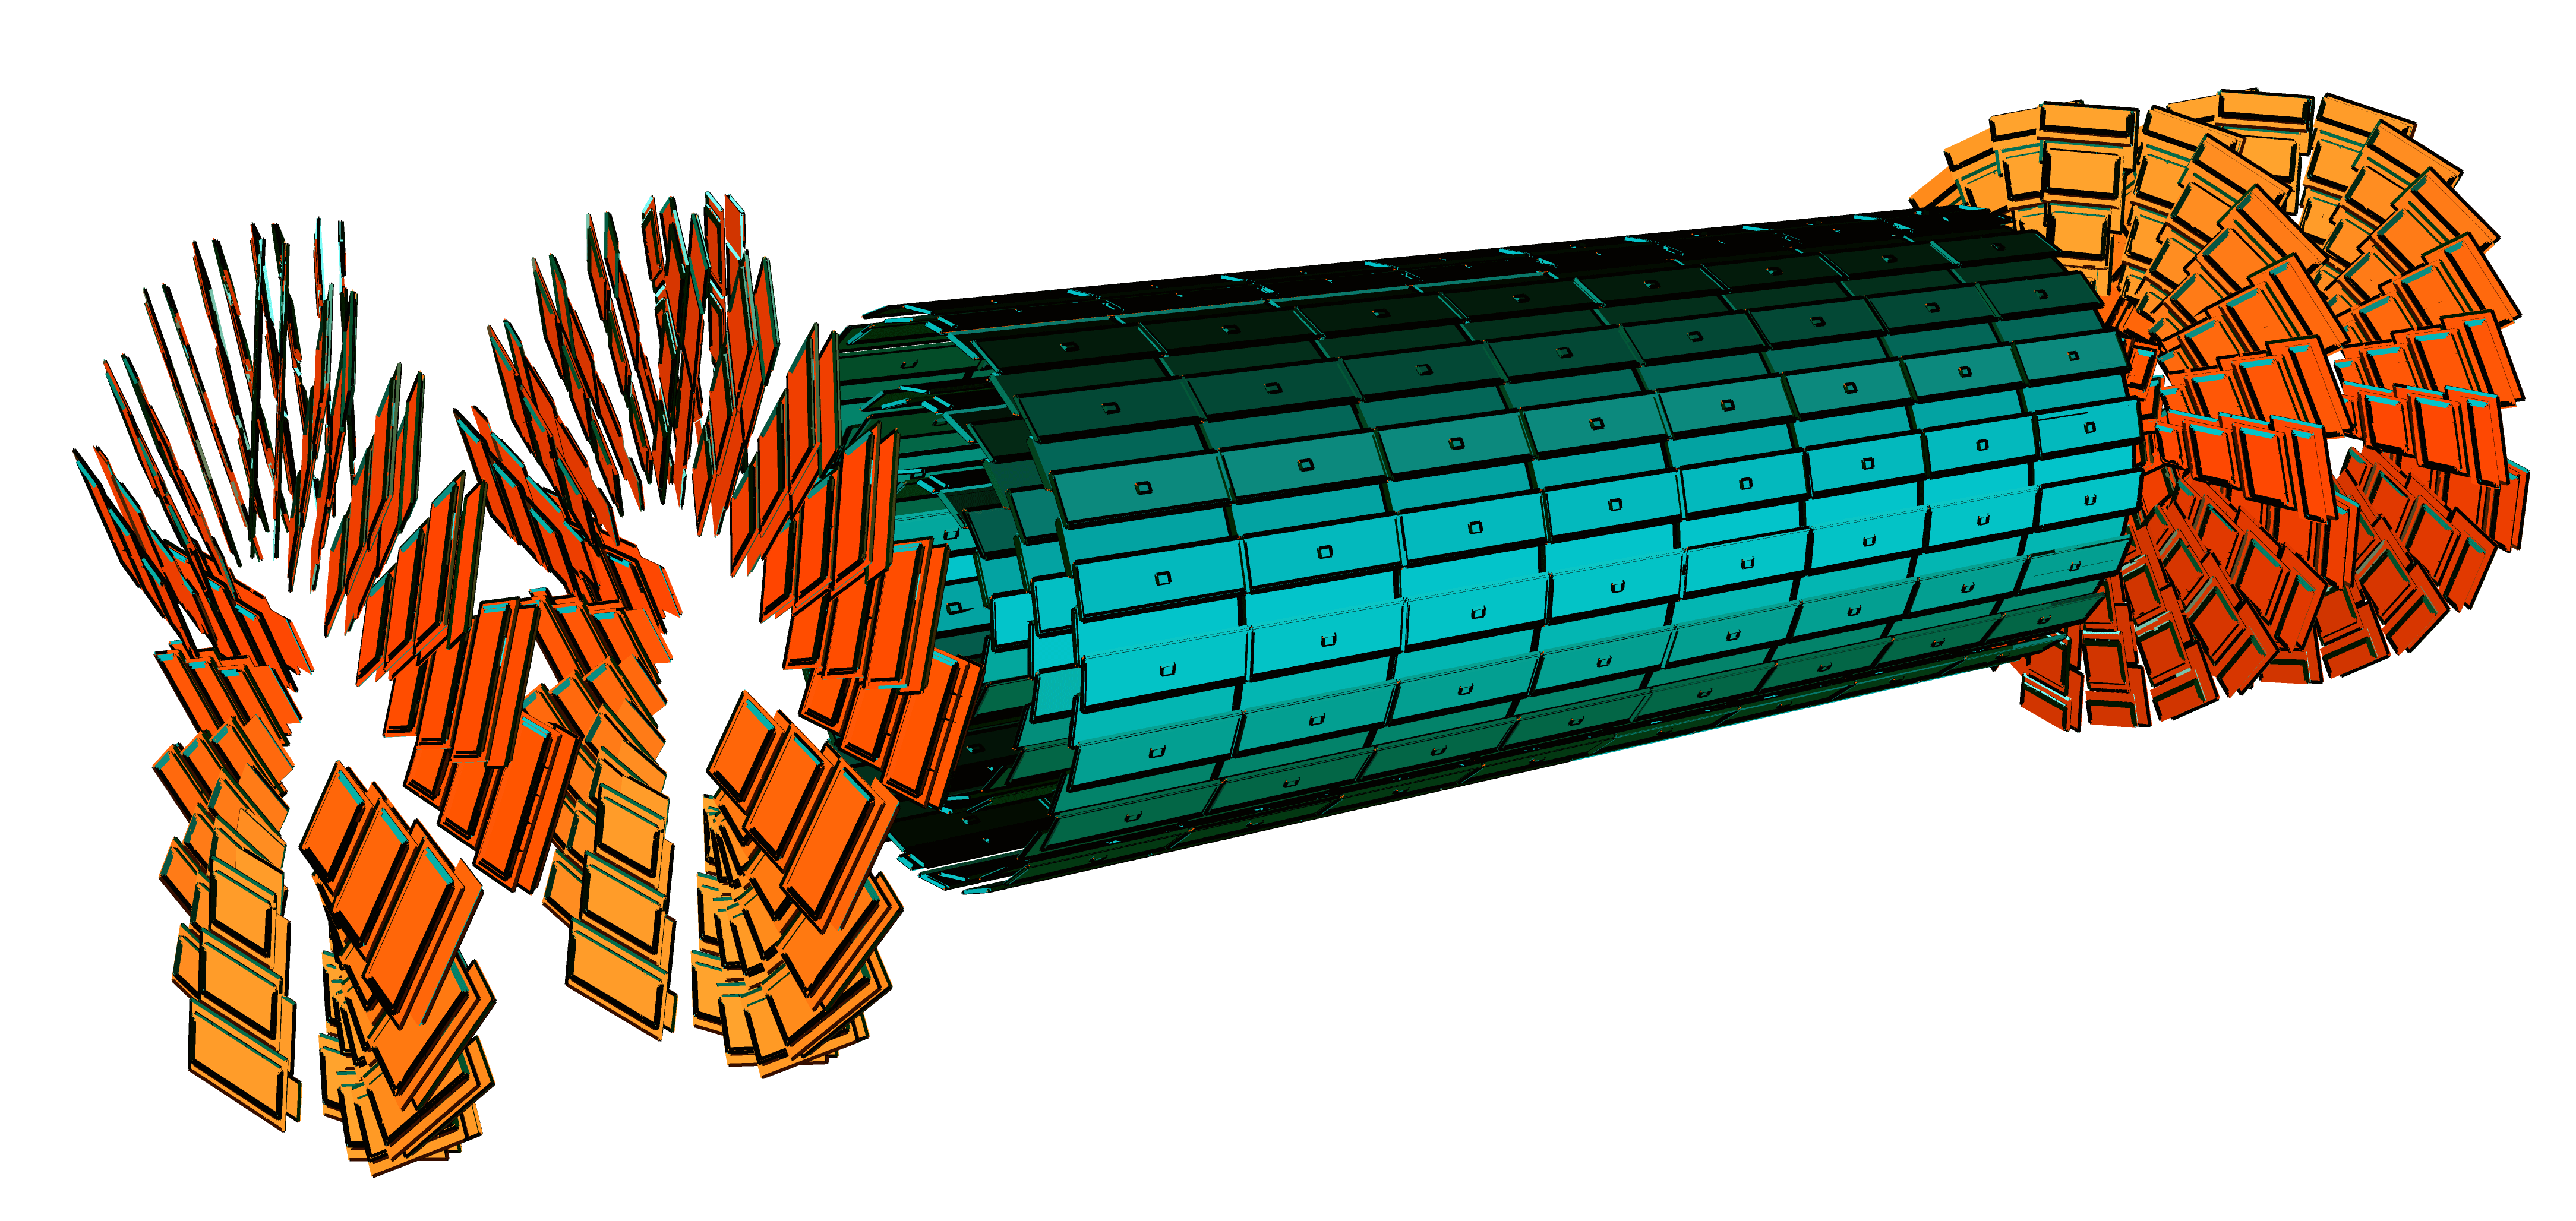
\includegraphics[width=10cm]{CMS_chapter_plots/pixel2}
  \caption{Pixel Detector \label{fig:pixel}}
\end{figure}

\paragraph{Silicon Strips}

The SST consists of four main subsystems, shown in \cref{fig:strip}
: the four-layer Tracker Inner Barrel (TIB), the six-layer Tracker Outer Barrel (TOB) and, on each side of the barrel region, the three-disk Tracker Inner Disks (TID), and the nine-disk Tracker End Caps (TEC).

Each TID disk is made of three rings of modules, while TEC disks have seven rings. The whole SST has a diameter of \unit[2.4]{m} and a length of \unit[5.5]{m}, being the largest silicon detector ever built with an active area of \unit[198]{m$^{2}$}. Its acceptance ranges over a region in pseudo-rapidity $\left| \eta\right|$ < 2.5.

This part of the tracker consist of 15 148 detector
modules and comprises 9.3 million detector channels. Each detector module consists of a carbon or graphite fibre frame, which supports the silicon sensor and the associated front-end readout electronics.
 
The silicon detectors work in much the same way as the pixels: as a charged particle crosses the material it knocks electron from atoms and within the applied electric field these move giving a very small pulse of current lasting a few nanoseconds. This small amount of charge is then amplified by APV25 chips, giving us "hits" when a particle passes, allowing us to reconstruct its path.

The charge on each microstrip is read out and amplified by an Analogue Pipeline Voltage (APV25) chip. Four or six such chips are housed within a “hybrid”, which also contains electronics to monitor key sensor information, such as temperature, and provide timing information in order to match “hits” with collisions. The APV25 stores the signals in a memory for several microseconds and then processes them before sending to a laser to be converted into infrared pulses.


\begin{figure}[H]
  \centering
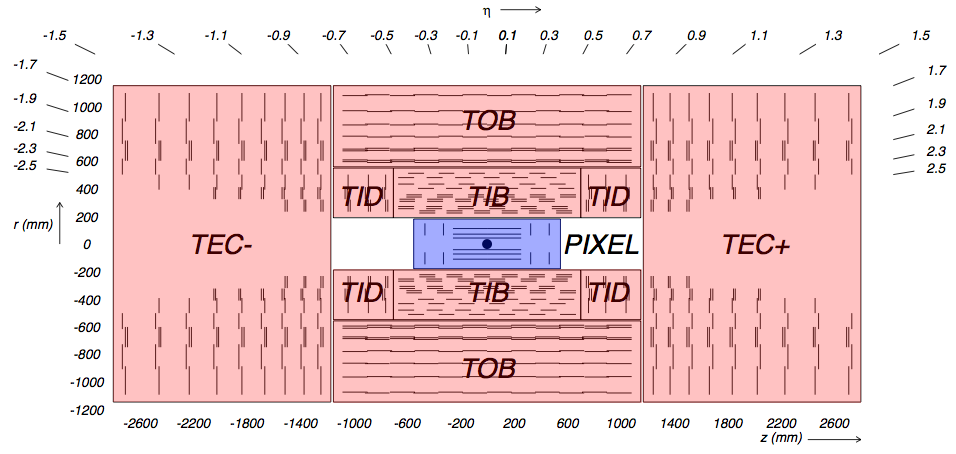
\includegraphics[width=10cm]{CMS_chapter_plots/strip}
  \caption{Strip and Pixel Detector \label{fig:strip}}
\end{figure}

\subsubsection{Electromagnetic Calorimeter (ECAL)}

The ECAL is divided into sections; a barrel section and two endcap sections. The barrel covers the pseudo-rapidity region $\eta$ < 1.48 and is constructed from 61200 lead tungstate crystals. The
crystals are grouped into units, called supermodules, of 1700 crystals. There are 36 supermodules in the barrel.

The endcaps cover the pseudo-rapidity region 1.48 < $\eta$ < 3.0. Each endcap is made from two ‘Dees’ and 7244 crystals. The crystals are grouped into modules of 25 crystals, known as supercrystals. The inner and outer boundaries of the endcaps are made more circular by the addition of smaller units known as partial supercrystals.

\begin{figure}[H]
  \centering
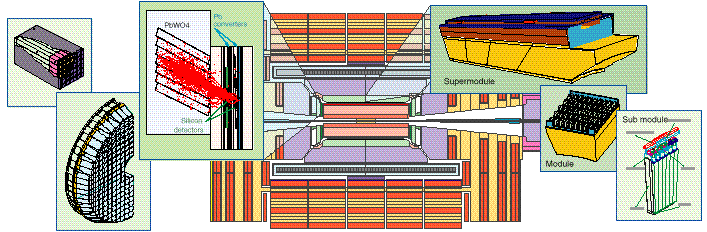
\includegraphics[width=14cm]{CMS_chapter_plots/caloc}
  \caption{Electromagnetic Calorimeter \label{fig:caloc}}
\end{figure}
\noindent
Lead tungstate (PbWO4) is a dense, fast and radiation-tolerant scintillating crystal. These three properties of the crystal make it an ideal choice for the CMS ECAL. The short radiation length and small Moliere radius allow a compact calorimeter to be constructed. The scintillation decay time is very fast with 80$\%$ of the scintillation light collected within 25ns (in the LHC bunches of protons collide every 25ns). 

\subsubsection{Hadronic Calorimeter (HCAL)}

The HCAL \cite{HCAL} is a sampling calorimeter which finds a particle’s position, energy and arrival time using alternating	 layers of "absorber" and fluorescent "scintillator" materials that produce a rapid light pulse when the particle passes through.

Special optic fibres collect up this light and deliver it into readout boxes where photodetectors amplify the signal. When the amount of light in a given region is summed up over many layers of tiles in depth, called a "tower", this total amount of light is a measure of a particle’s energy. 

The hadron calorimeter barrel is radially restricted between the outer extent of the electromagnetic calorimeter (R = 1.77 m) and the inner extent of the magnet coil (R = 2.95 m). This constrains the total amount of material which can be put in to absorb the hadronic shower. Therefore, an outer hadron calorimeter is placed outside the solenoid complementing the barrel calorimeter. Beyond $|\eta| = 3$, the forward hadron calorimeters placed at 11.2 m from the interaction point extend the pseudorapidity coverage down to $|\eta| = 5.2$. 

The HCAL is organized into barrel (formed by two sections : Hadron Barrel(HB) in the region $|\eta|$ < 1.4 and Hadron Outer (HO) in the region $|\eta|$ < 1.26), Hadron Endcap (HE) [1.3<$|\eta|$ < 3.0]  and Hadron Forward (HF) [2.9<$|\eta|$ < 5.0]  sections.(Fig. \ref{fig:hcal1})
\begin{figure}[H]
  \centering
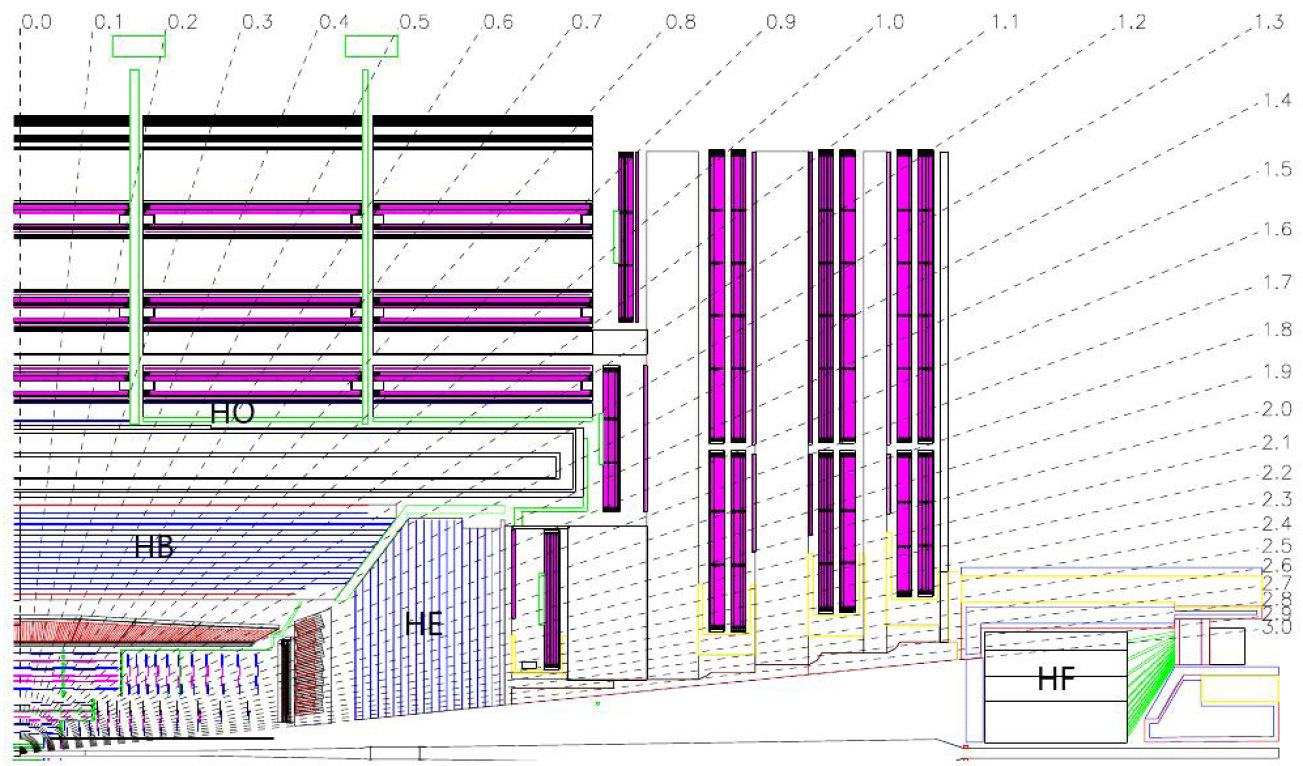
\includegraphics[width=9cm]{CMS_chapter_plots/hcal1}
  \caption{Longitudinal view of the CMS detector showing the locations of the hadron barrel
  (HB), endcap (HE), outer (HO) and forward (HF) calorimeters. \label{fig:hcal1}}
\end{figure}

The HB is a sampling calorimeter covering the pseudorapidity range $|\eta|$ < 1.4, resulting in 2304 towers with a segmentation $\Delta\eta\times\Delta\phi=0.087\times 0.087$.
The HB consists of 36 identical azimuthal wedges which form the two half-barrels (HB$+$ and HB$-$).
\begin{figure}[H]
  \centering
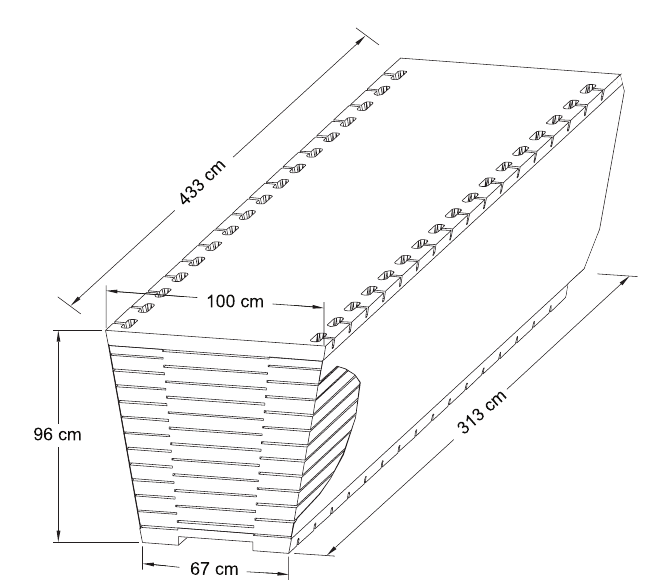
\includegraphics[width=8cm]{CMS_chapter_plots/hcal3}
  \caption{View of an HB wedge. \label{fig:hcal3}}
\end{figure}

The wedges (Fig. \ref{fig:hcal3}) are constructed out of flat brass absorber plates aligned parallel to the beam axis.
The HB baseline active material is 3.7 mm thick Kuraray SCSN81 plastic scintillator, chosen for its long term stability and moderate radiation hardness.

The granularity of the HCAL is 25 times coarser than that of
the ECAL, which would not allow charged and neutral hadrons to be spatially separated in jets with a transverse momentum much above 100 GeV/c. The hadron energy resolution in the combined ECAL-HCAL system is, however, of the order of 10$\%$ at 100 GeV. This resolution allows neutral hadrons to be detected as an energy excess on top of the energy deposited by the charged hadrons pointing to the same calorimeter cells.

More details about the Hadronic Calorimeter may be found in \cite{HCAL2, HCAL3, HCAL4, HCAL5}.

\subsubsection{The Muon System}
\noindent Quality muon detection is one of CMS's most important function. From its earliest conceptual stages, robust and precise muon detection has been the central theme.

Muons can penetrate several metres of iron without interacting. Unlike most particles they are not stopped by any of CMS's calorimeters ($\tau \approx$ 2.2 $\mu$s). Therefore, chambers to detect muons are placed at the very edge of the experiment where they are the only particles likely to register a signal. 

\noindent
The CMS muon system is designed to have the capability of reconstructing the momentum and charge of muons over the the entire kinematic range of the LHC. 

\noindent
The Muon system is a type of tracking detector, and is divided in two main regions: the Barrel ($|\eta|$< 1.2) and  the endcap (1.2 <$|\eta|$< 2.4).\\
There are three types of detectors in the Muon System:

\paragraph{Drift Tubes (DT)}
The drift tube (DT) chamber (Fig. \ref{fig:DT}) system measures muon positions in the barrel part of the detector.

The chamber volume is filled with a Ar(85 $\%$)/CO$_{2}$(15 $\%$) gas mixture, kept at atmospheric pressure.  When a muon or any charged particle passes through the volume, it knocks electrons off the atoms of the gas. By registering where along the wire electrons hit, as well as by calculating the muon's original distance away from the wire, DTs give two coordinates for the muon’s position.
\begin{figure}[H]
  \centering
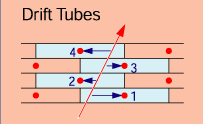
\includegraphics[width=6cm]{CMS_chapter_plots/DT}
  \caption{Muon Drift Tubes \label{fig:DT}}
\end{figure}
\paragraph{Cathode Strip Chamber (CSC)}
Cathode strip chambers (CSC) are used in the endcap disks where the magnetic field is inhomogeneous and particle rates are high.

CSCs consist of arrays of positively charged "anode" wires crossed with negatively charged copper "cathode" strips within a gas volume.

When muons pass through, they knock electrons off the gas atoms, which flock to the anode wires creating an avalanche of electrons. Positive ions move away from the wire and towards the copper cathode, also inducing a charge pulse in the strips, at right angles to the wire direction.
\begin{figure}[H]
  \centering
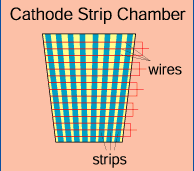
\includegraphics[width=5cm]{CMS_chapter_plots/CSC}
  \caption{Cathode Strip Chamber \label{fig:CSC}}
\end{figure}

\paragraph{Resistive Plate Chambers (RPC)}
Resistive plate chambers (RPC) are fast gaseous detectors that provide a muon trigger system parallel with those of the DTs and CSCs.

RPCs consist of two parallel plates, a positively-charged anode and a negatively-charged cathode, both made of a very high resistivity plastic material and separated by a gas volume.

When a muon passes through the chamber, electrons are knocked out of gas atoms. These electrons in turn hit other atoms causing an avalanche of electrons. The electrodes are transparent to the signal (the electrons), which are instead picked up by external metallic strips after a small but precise time delay. The pattern of hit strips gives a quick measure of the muon momentum, which is then used by the trigger to make immediate decisions about whether the data are worth keeping. 

RPCs combine a good spatial resolution with a time resolution of just one nanosecond (one billionth of a second).
\begin{figure}[H]
  \centering
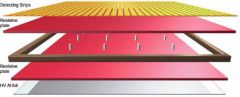
\includegraphics[width=5cm]{CMS_chapter_plots/RPClayers}
  \caption{Resistive Plate Chambers \label{fig:RPClayers}}
\end{figure}


In total there are 1400 muon chambers: 250 drift tubes (DTs) and 540 cathode strip chambers (CSCs) track the particles’ positions and provide a trigger, while 610 resistive plate chambers (RPCs) form a redundant trigger system, which quickly decides to keep the acquired muon data.

The Barrel Detector consists of 4 concentric “stations” (Fig. \ref{fig:mustations}) of 250 chambers inside the magnet return yoke of CMS, which is in turn divided into 5 wheels. Each wheel is divided into 12 sectors, each covering a $30^{\circ}$ azimuthal angle.

The 2 innermost stations, named MS1 and MS2, consist of “sandwiches” made of a DT chamber placed between 2 RPCs. The 2 outermost stations, MS3 and MS4, consist of packages of a DT chamber coupled to a layer made of 1, 2, or 4 RPCs, depending on the sector and station, placed on the innermost side of the station.

\begin{figure}[H]
  \centering
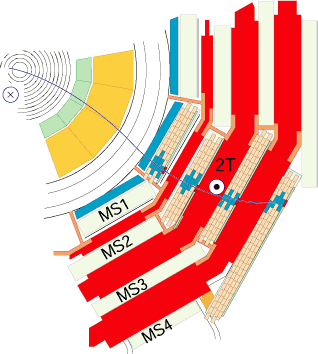
\includegraphics[width=6cm]{CMS_chapter_plots/mustations}
  \caption{Muons Stations \label{fig:mustations}}
\end{figure}

More information about the CMS Muon System may be found in \cite{MUON}.

\subsection{CMS Data Acquisition and Triggering}\label{triggerbase}

When CMS performs at its peak, about one billion proton-proton interactions will take place every second inside the detector. There is no way that data from all these events could be read out, and even if they could, most would be less likely to reveal new phenomena.

We therefore need a "trigger" \cite{TRIGGER1,TRIGGER2} that can select the potentially interesting events, and reduce the rate to just a few hundred "events" per second, which can be read out and stored on computer disk for subsequent analysis.

This task is performed by the trigger system, which is the start of the physics event selection process. The rate is reduced in two steps called Level-1 (L1) Trigger and High-Level Trigger (HLT), respectively. The Level-1 Trigger consists of custom-designed, largely programmable electronics, whereas the HLT is a software
system implemented in a filter farm of about one thousand commercial processors. The rate reduction capability is designed to be at least a factor of $10^{6}$ for the combined L1 Trigger and HLT. 

Level 1 of the trigger is an extremely fast and wholly automatic process that looks for simple signs of interesting physics, e.g. particles with a large amount of energy or in unusual combinations.

The Level 1 trigger select the best 100,000 events each second from the billion available. For the next test, the HLT assimilate and synchronise information from different parts of the detector to recreate the entire event and send it to a farm of more than 1000 standard computers.

\begin{figure}[H]
  \centering
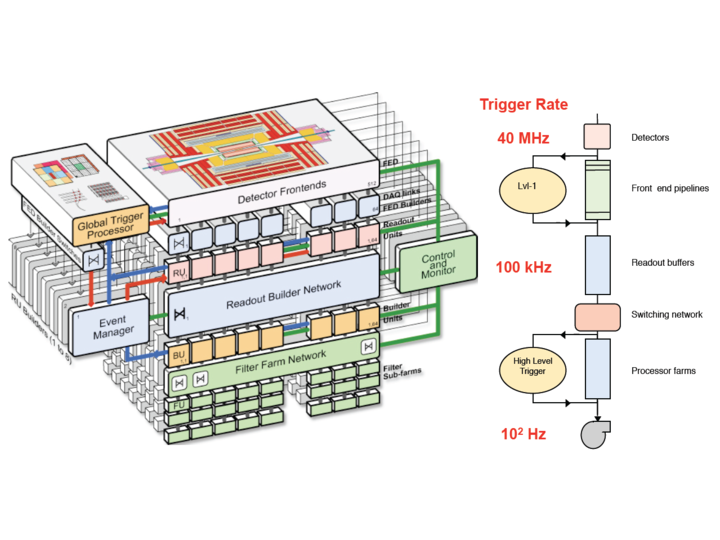
\includegraphics[width=14cm]{CMS_chapter_plots/TRIGGER}
  \caption{CMS Triggering System \label{fig:TRIGGER}}
\end{figure}

Overall they select 100 events per second and the remaining 99,900 are thrown out. We are left with only the collision events that might teach us something new about physics. 

\subsection{Computing and Software}

The CMS Computing Model \cite{COMPUTING} describes how computing centres available to CMS around the world are distributed and configured in a tiered architecture that functions as a single coherent system. It also describes how detector data and MC data travel through the tiers, and how data are distributed, stored, and accessed.

\paragraph{The CMS Data Hierarchy}
CMS Data is arranged into a hierarchy of data tiers. Each physics event is written into each data tier, where the tiers each contain different levels of information about the event. The three main data tiers written in CMS are:
\begin{itemize}
\item 
\textbf{RAW}: full event information from the Tier-0 (i.e. from CERN), containing "raw" detector information (detector element hits, etc)
RAW is not used directly for analysis
        
\item   
\textbf{RECO} ("RECOnstructed data"): the output from first-pass processing by the Tier-0. This layer contains reconstructed physics objects, but it's still very detailed RECO can be used for analysis, but is too big for frequent or heavy use when CMS has collected a substantial data sample.

\item   
\textbf{AOD} ("Analysis Object Data"): this is a condense version of the RECO event information, and is expected to be used for most analyses AOD provides a trade-off between event size and complexity of the available information to optimize flexibility and speed for analyses      
\end{itemize} 

     
\paragraph{CMSSW and Event Data Model (EDM)} 
The overall collection of software, referred to as CMSSW, is built around a Framework, an Event Data Model (EDM), and Services needed by the simulation, calibration and alignment, and reconstruction modules that process event data.

The CMSSW event processing model consists of one executable, called \textit{cmsRun}, and many plug-in modules which are managed by the Framework. All the code needed in the event processing (calibration, reconstruction algorithms, etc.) is contained in the modules. The same executable is used for both detector and Monte Carlo data.

The CMSSW executable, cmsRun, is configured at run time by the user's job-specific configuration file. This file tells cmsRun:

\begin{itemize}
\item 
which data to use
\item 
which modules to execute
\item
which parameter settings to use for each module
\item
what is the order or the executions of modules, called path
\item
how the events are filtered within each path, and
\item
how the paths are connected to the output files 
\end{itemize}

Unlike the previous event processing frameworks, cmsRun is extremely light:only the required modules are dynamically loaded at the beginning of the job.

The CMS Event Data Model (EDM) is centered around the concept of an Event. An Event is a C++ object container for all RAW and reconstructed data related to a particular collision. During processing, data are passed from one module to the next via the Event, and are accessed only through the Event. All objects in the Event may be individually or collectively stored in ROOT files, and are thus directly browsable in ROOT. This allows tests to be run on individual modules in isolation. 


\chapter{General description of the physics objects}

\section{Track reconstruction}

Under nominal conditions of the LHC at $\sqrt{s}=13$ TeV a typical instantaneous luminosity around $\designlumi$ is expected, with the proton bunches intersecting at intervals of 25 ns. Therefore, the CMS tracker will be cross by about 1000 charged particles at each bunch crossing, producing an average of more than twenty proton-proton (pp) collisions. These multiple interactions are known as \emph{pileup} \cite{1742-6596-404-1-012045}, to which prior or later bunch crossings can also contribute because of the finite time resolution of the detector.

The first step in processing the data prior to track reconstruction is the efficient detection of \emph{hits},
which represent the positions in the sensors of the tracker where charged particles passed through.
Track reconstruction is the process of using the hits on the pixel (section \ref{pixel}) and strip tracker (section \ref{strip}) to estimate the momentum and the position parameters (the longitudinal $z_{0}$ and transverse $d_{0}$ distances relative to the beam axis) of the charged particles responsible for the hits (tracks). Figure \ref{fig:tracks_par} shows the position parameters of a track.

\begin{figure}[H]
  \caption{
 Geometrical description of the closest approach point of a track (curved line) to the beam line:  transverse ($d_{0}$) and longitudinal ($z_{0}$) impact parameters.
    \label{fig:tracks_par}}
  \centering
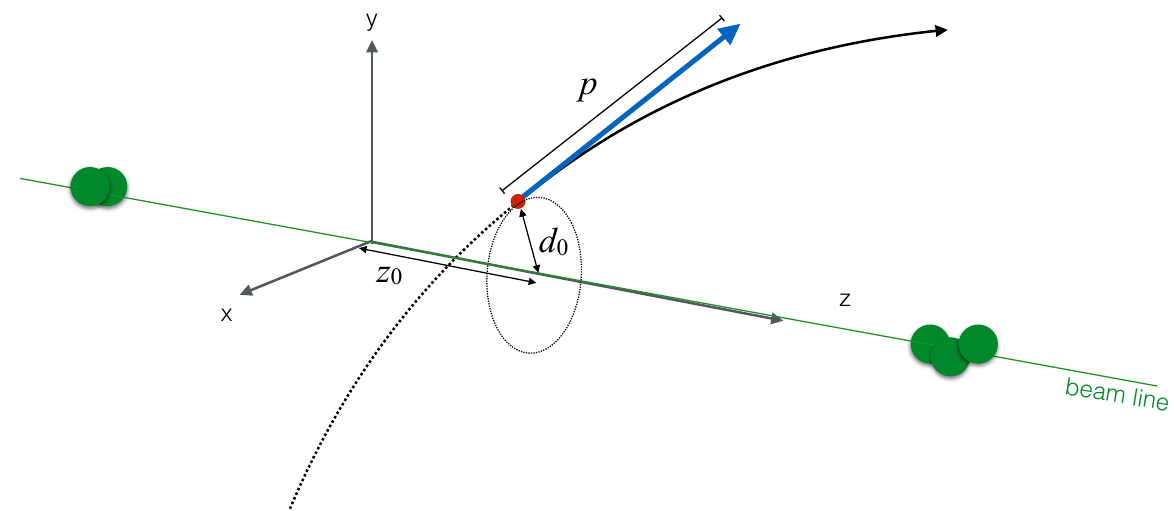
\includegraphics[width=15cm]{Chapter3_plots/trackpar.pdf}
\caption*{Source: Andreas Salzburger \cite{Bortolleto}.}
\end{figure}

%In the quasi-uniform magnetic field of the tracker, charged particles follow helical paths and therefore five parameters are needed to define a trajectory. Three pixel hits (triplet) are used to form a track, from which the transverse momentum, the longitudinal $z_{0}$ and transverse $d_{0}$ impact parameters (IP) are computed.
Reconstructing the trajectories of charged particles is a computationally challenging task. Hence, CMS developed a software, which support pattern recognition and track fitting in the same framework, called \emph{Combinatorial Track Finder} (CTF) \cite{Chatrchyan:2014fea}.
This software is based on an adaptation of the \emph{Combinatorial Kalman filter} method \cite{Billoir:1989mh,Billoir:1990we,Mankel:1997dy}, which in turn is an extension of the \emph{Kalman filter} method \cite{Fruhwirth:1987fm}.  

The collection of reconstructed tracks is produced by multiple passes (iterations) of the CTF track
reconstruction sequence, in a process called \emph{iterative tracking}. 
The idea behind iterative tracking is to search in the initial iterations for the easiest tracks to find (e.g., of relatively large $\pt$, and produced near the interaction region). After each iteration, the hits related with tracks are removed in a search
for more difficult classes of tracks (e.g., low-$\pt$, or greatly displaced tracks).
Each iteration process contains four steps:

%\begin{figure}[H]
%  \centering
%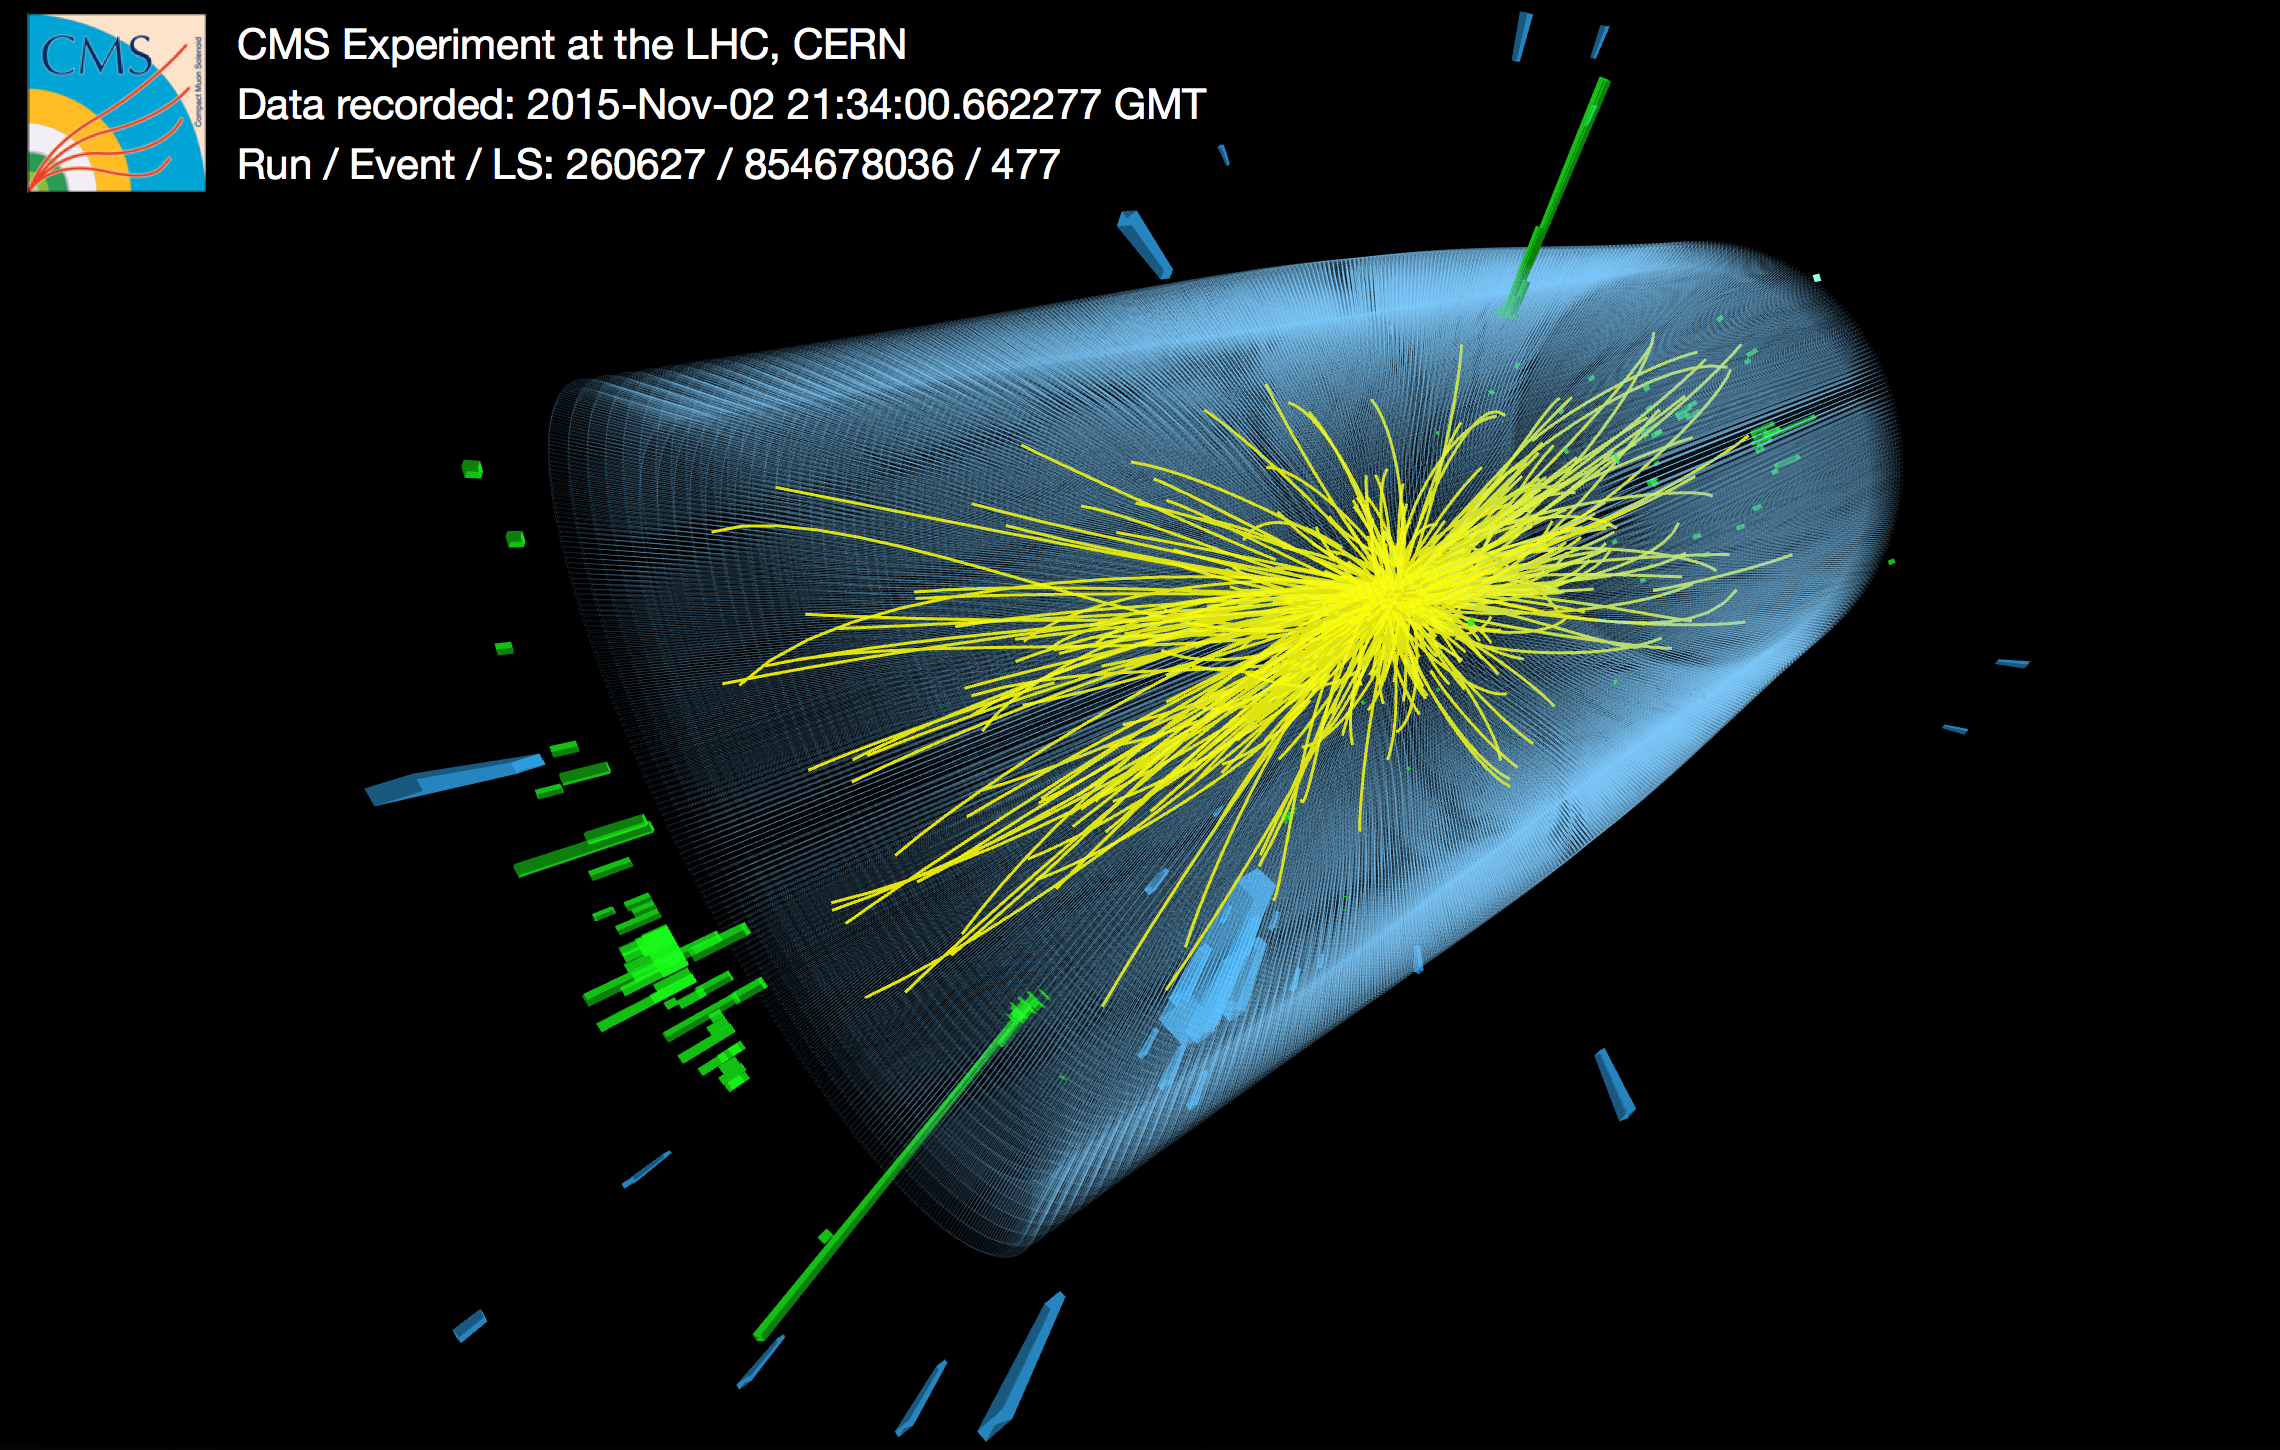
\includegraphics[width=10cm]{Chapter3_plots/tracks_display}
%  \caption{
%  A typical event display of a 13 TeV proton-proton collision observed by the CMS in 2015. The yellow lines are the measured tracks of charged particles produced in the collision.
%    \label{fig:tracks_display}}
%\end{figure}
\begin{itemize}
\item 
Seed generation provides initial track candidates found using only a few (2 or 3) hits. A seed
defines the initial estimate of the trajectory parameters and their uncertainties
\item
Track finding is based on a Kalman filter. It extrapolates the seed trajectories along the
expected flight path of a charged particle, searching for additional hits that can be assigned
to the track candidate.
\item
The track-fitting module is used to provide the best possible estimate of the parameters of
each trajectory by means of a Kalman filter and smoother.
\item
Track selection sets quality flags, and discards tracks that fail certain specified criteria
\end{itemize}

Muons are reconstructed better than any other charged particle in the tracker, as they mainly
interact with the silicon detector through ionization of the medium and, unlike electrons, their
energy loss through bremsstrahlung is negligible. Muons therefore tend to cross the entire volume
of the tracking system, producing detectable hits in several sensitive layers of the detector.
For isolated muons with $1 < \pt < 100$ GeV, the tracking efficiency is $>$99$\%$ over the full $\eta$-range of tracker acceptance,
and does not depend on $\pt$ as shown in Fig.\ref{fig:trackeff}. The fake rate is completely negligible.

\begin{figure}[!ht]
\caption{
Track reconstruction efficiencies for single isolated muons passing high-purity quality requirements. Results are shown as a function of $\eta$ (left), for $\pt$ = 1, 10, and 100 GeV. They are also shown as a function of $\pt$ (right), for the barrel, transition, and
endcap regions, which are defined by the $\eta$ intervals of 0–0.9, 0.9–1.4 and 1.4–2.5, respectively. 
}
\begin{tabular}{cc}
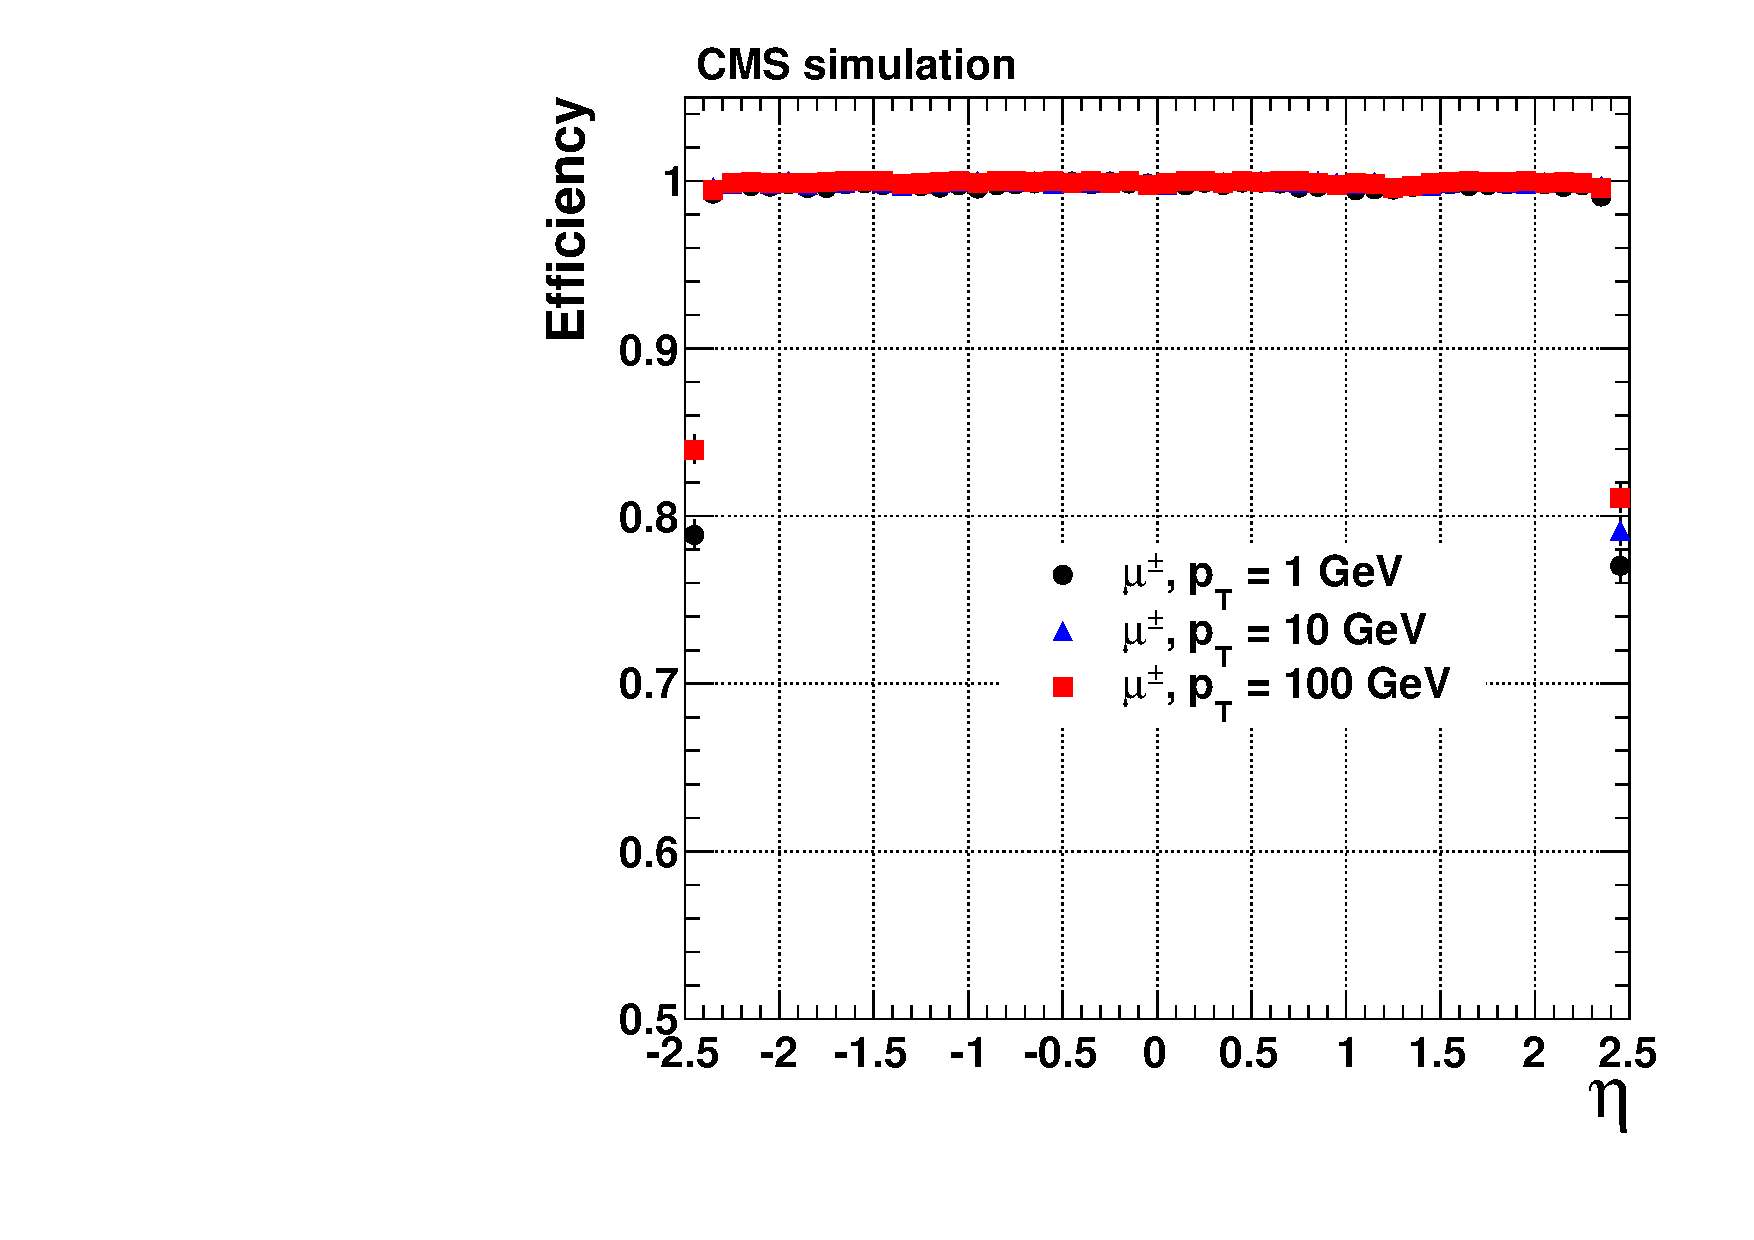
\includegraphics[width=7cm]{Chapter3_plots/CMS-TRK-11-001_Figure_008-a} &
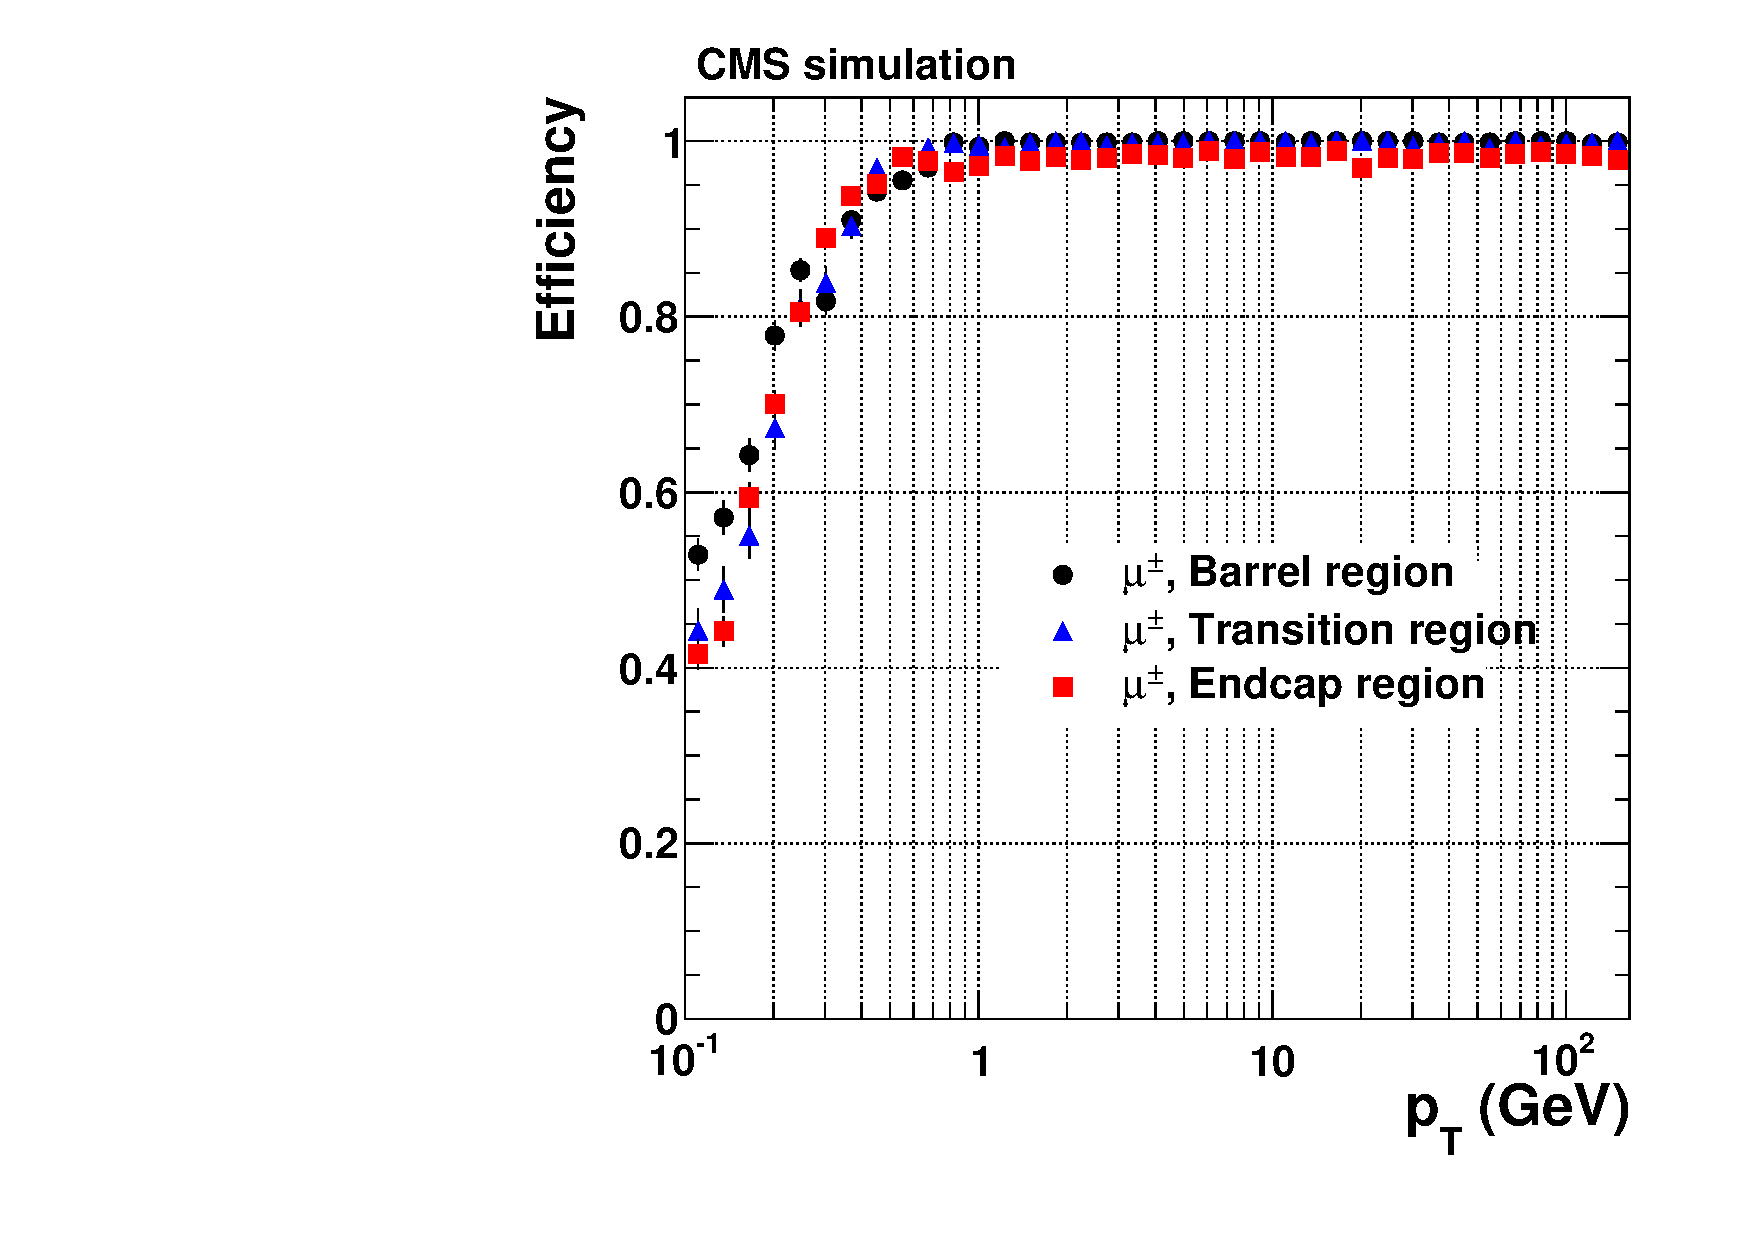
\includegraphics[width=7cm]{Chapter3_plots/CMS-TRK-11-001_Figure_008-b} \\
\end{tabular}
\caption*{Source: CMS Collaboration, JINST, vol. 9, no. 10, p. P10009, 2014.}
\label{fig:trackeff}
\end{figure}

\section{Primary Vertex (PV) }

The objective of primary-vertex reconstruction is to determine the location, and the related uncertainty, of all proton-proton (pp) interaction vertices in each event, including vertices originated from the primary event or from additional pp interactions (pileup), using the available reconstructed tracks. The method consists of three steps:
\begin{itemize}
\item
Selection of the tracks
\item
Clustering of the tracks that appear to originate from the same
interaction vertex
\item
Fitting for the position of each vertex using its associated tracks
\end{itemize}

Tracks are selected if they are produced rapidly in the primary interaction region. The selected tracks are clustered based on information from their z-coordinates and  their point of closest approach to the centre of the beam spot. Track clustering is performed using a deterministic annealing (DA) algorithm \cite{Rose}, finding the global minimum for a problem with many degrees of freedom.
After identifying candidate vertices based on the DA clustering, the candidates with at least two tracks are then fitted using an adaptive vertex fitter \cite{Fruhwirth:1027031} to compute the best estimate of vertex parameters (position, covariance matrix, number of degrees of freedom for the vertex, and weights of the tracks used in the vertex). 

%To identify and reject the beam background events, various methods have been investigated.
%Requiring that the event have a high quality primary vertex very close to the nominal inter-
%action point is a powerful rejection technique. The primary vertex is required to have at least
%four degrees of freedom, to be no more than 2 cm in the radial direction and 15 cm in the beam
%direction away from the nominal interaction point. This method provides a very clean sample
%of real proton-proton collision events. The purity of the sample can be evaluated by investigat-
%ing the distributions in Fig. 13 which shows the number of tracks and number of pixel clusters
%in 7 TeV colliding and non-colliding beams, before and after applying the primary vertex se-
%lection. The distributions of tracks and pixel clusters from colliding beams exhibit long tails
%which are not compatible with expectations from simulation.

%In the adaptive vertex fit, each track in the vertex is assigned a weight between 0 and 1, which reflects the likelihood that it genuinely belongs to the vertex. Tracks that are consistent with the position of the reconstructed vertex have a weight
%close to 1, whereas tracks that lie more than a few standard deviations from the vertex have small
%weights. The number of degrees of freedom in the fit is defined as

%\begin{eqnarray}
%n_{\text{dof}} = -3 +2 \sum_{i=1}^{\# \text{tracks} } w_{i} 
%\end{eqnarray}

%where $w_{i}$ is the weight of the ith track, and the sum runs over all tracks associated with the vertex.
%The value of $n_{\text{dof}}$ is therefore strongly correlated with the number of tracks compatible with arising
%from the interaction region. For this reason, $n_{\text{dof}}$can be also used to select true proton-proton
%interactions
 
The primary-vertex efficiency is estimated to be close to 100$\%$ when more than two tracks are used to reconstruct the vertex. Figure \ref{fig:PVeff} shows the efficiency of the primary-vertex reconstruction as a function of the number of tracks clustered in $z$. The effect of pileup on the efficiency is checked using simulated minimum-bias events, with and without added pileup, and the loss of efficiency is found to be $<$ 0.1$\%$ for the pileup with a mean value of 8 \cite{CMS:2010wta}.

\begin{figure}[!ht]
  \caption{
Primary-vertex reconstruction efficiency as a function of the number of tracks in a cluster, measured in minimum-bias data and in MC simulation.
}
  \centering
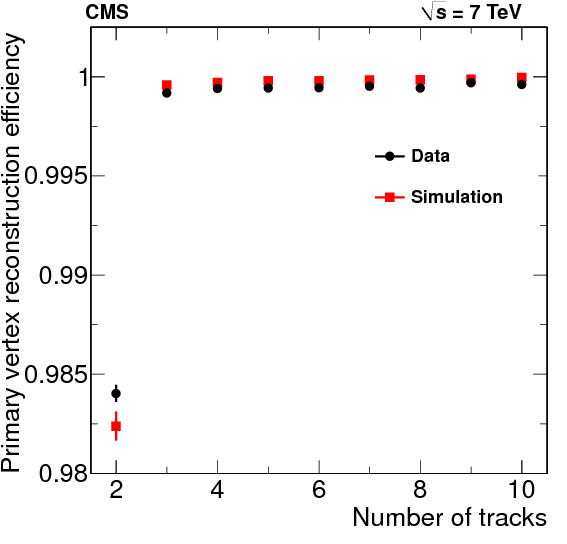
\includegraphics[width=7cm]{Chapter3_plots/PV_efficiency}
\caption*{Source: CMS Collaboration, JINST, vol. 9, no. 10, p. P10009, 2014.}
\label{fig:PVeff}
\end{figure}




%\begin{figure}[H]
%  \centering
%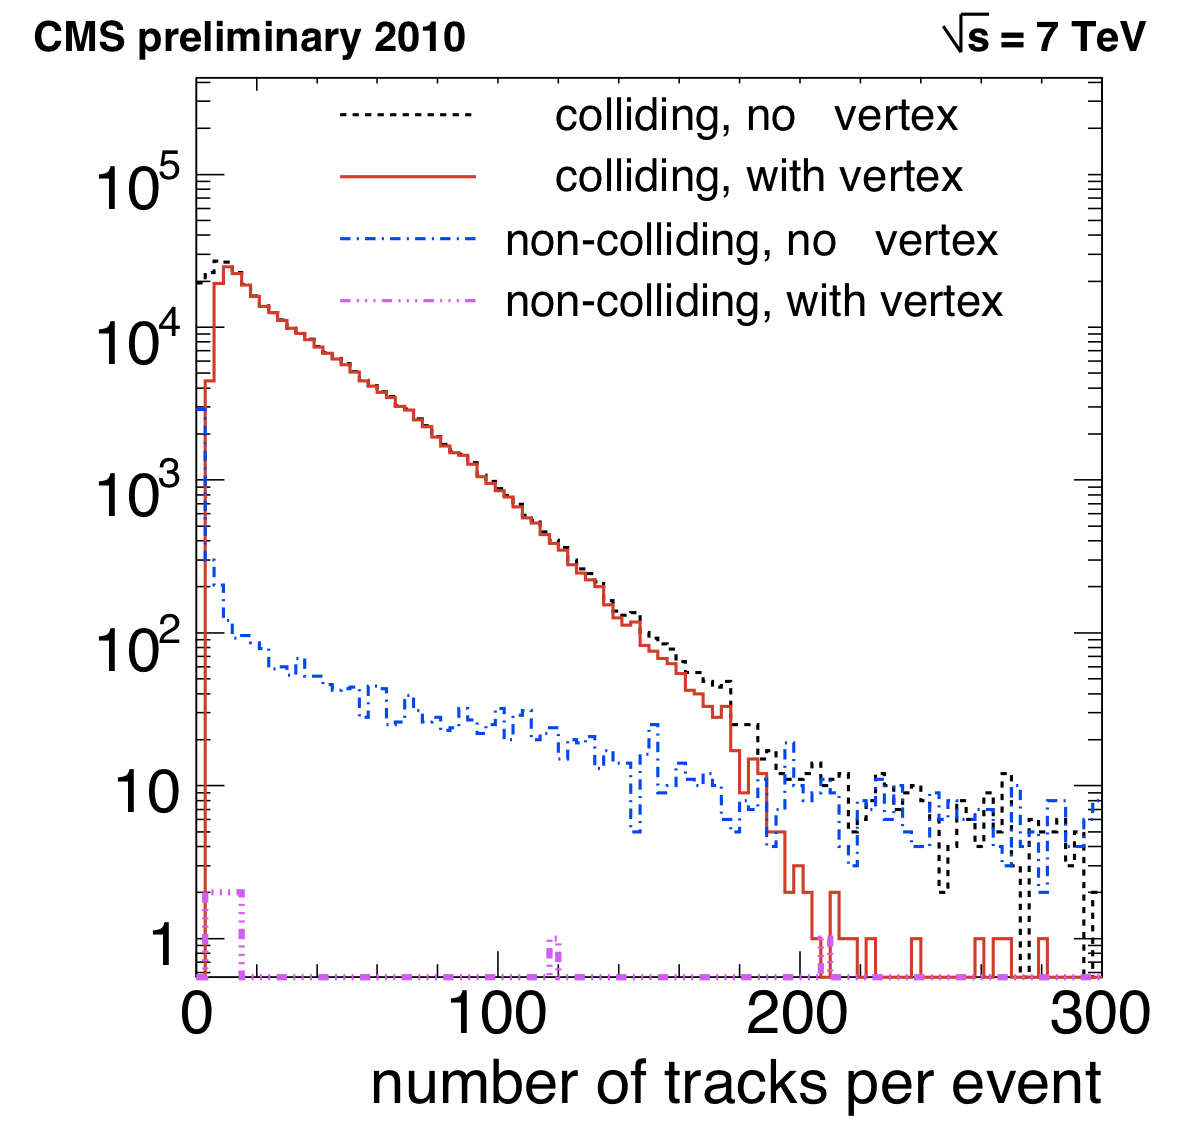
\includegraphics[width=10cm]{Chapter3_plots/numberoftracks}
%  \caption{Distributions of number of tracks per event. Collision events before primary vertex selection are shown as dashed (black) line
%  while collision events after primary vertex selection are shown as solid (red) line. Non-colliding
%  beam events before primary vertex selection are shown as dot-dashed (blue) line while non-
%  colliding beam events after primary vertex selection are shown as triple-dot-dashed (magenta)
%  line.  \label{fig:tracks}}
%\end{figure}


\section{Particle Flow (PF) }

The global event reconstruction (also called particle-flow event reconstruction reside in the reconstruction and identification of each single particle with an optimized combination of all subdetector information. In this process, the identification of the particle type (photon, electron, muon, and hadrons) plays an important role in the determination of the particle direction and energy.
 
\begin{itemize}
 \item \textbf{Photons}
(\eg coming from \Pgpz  decays or from electron bremsstrahlung) are identified as ECAL energy clusters not linked to the extrapolation of any charged particle trajectory to the ECAL. The energy of photons is directly obtained from the ECAL measurement, corrected for zero-suppression effects.

\item \textbf{Electrons} 
(\eg coming from photon conversions in the tracker material or from \cPqb-hadron semileptonic decays) are identified as a primary charged particle track and potentially many ECAL energy clusters corresponding to this track extrapolation to the ECAL and to possible bremsstrahlung photons emitted along the way through the tracker material. The energy of electrons is determined from a combination of the track momentum at the main interaction vertex, the corresponding ECAL cluster energy, and the energy sum of all bremsstrahlung photons attached to the track.

\item \textbf{Muons}
 (\eg from \cPqb-hadron semileptonic decays) are identified as a track in the central tracker consistent with either a track or several hits in the muon system, associated with an energy deficit in the calorimeters. The energy of muons is obtained from the corresponding track momentum.
 
\item \textbf{Charged hadrons} 
are identified as charged particle tracks neither identified as electrons, nor as muons. The energy of charged hadrons is determined from a combination of the track momentum and the corresponding ECAL and HCAL energy, corrected for zero-suppression effects and for the response function of the calorimeters to hadronic showers.

\item \textbf{Neutral hadrons}
are identified as HCAL energy clusters not linked to any charged hadron trajectory, or as ECAL and HCAL energy excesses with respect to the expected charged hadron energy deposit. The energy of neutral hadrons is obtained from the corresponding corrected ECAL and HCAL energy.
\end{itemize}

\begin{figure}[htp]
\caption{A slice through the CMS detector. CMS consists of a central silicon Tracker (Pixel and Strips), an Electromagnetic Calorimeter, a Hadron Calorimeter, a Superconduction Solenoid Magnet, a massive iron return yoke instrumented with Muon Chambers. The depicted interactions present an ideal detector behavior for the
different particles $\mu$ , $e$, charged and neutral hadrons, and $\gamma$.}
  \centering
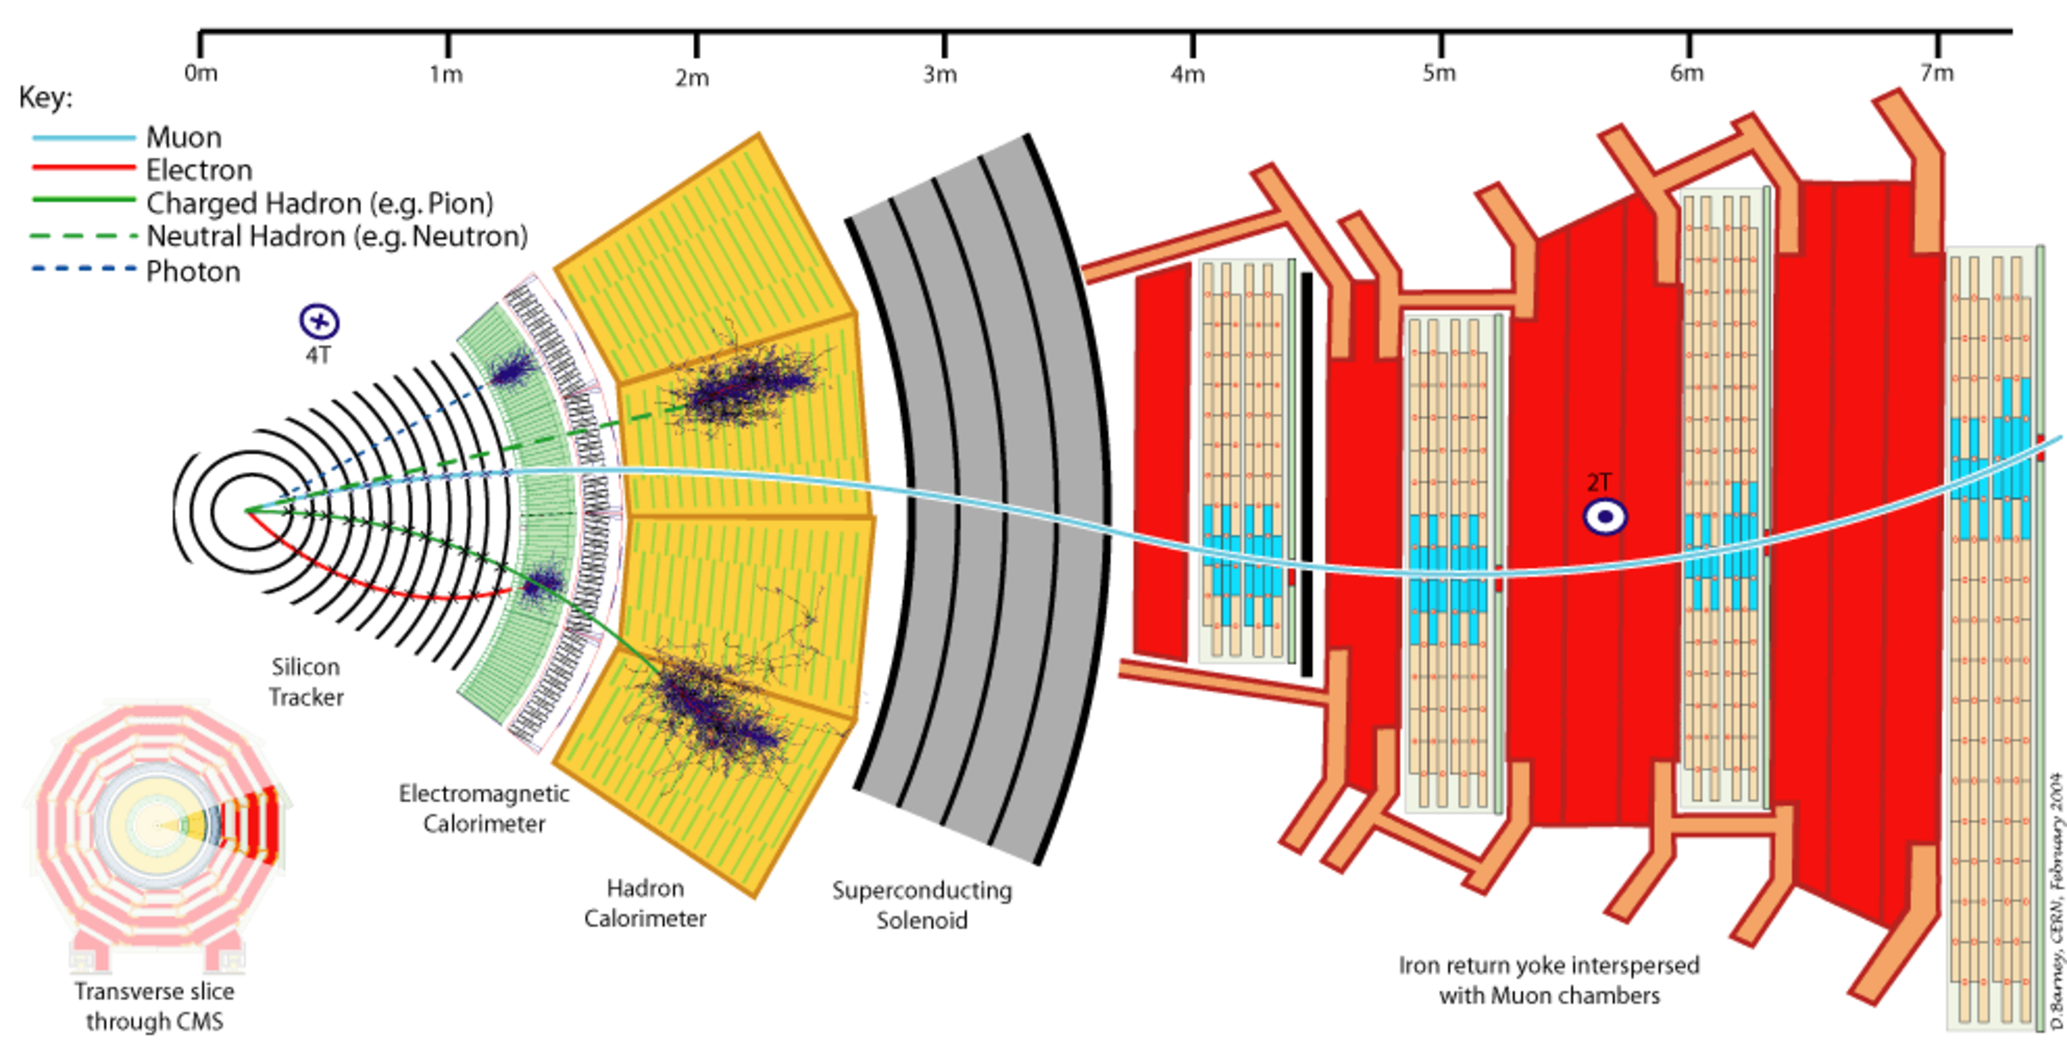
\includegraphics[width=16cm]{CMS_chapter_plots/CMS_Slice}
\label{figure}
\caption*{Source: CMS-PHO-GEN-2016-001, \cite{Barney:2120661}}
\end{figure}

\section{Jets }\label{aniktlab}

Jets are the experimental signatures of quarks and gluons produced in high-energy processes such as hard scattering of partons in proton-proton collisions. The LHC collides protons containing colored partons: quarks, antiquarks and gluons. Almost immediately after being produced, a quark or gluon fragments and hadronises, leading to a collimated spray of energetic hadrons: a jet (Fig. \ref{jet1figure} ).
\begin{figure}[H]
\caption{pp-collision resulting in a collimated spray of particles, a jet. \label{jet1figure}}
  \centering
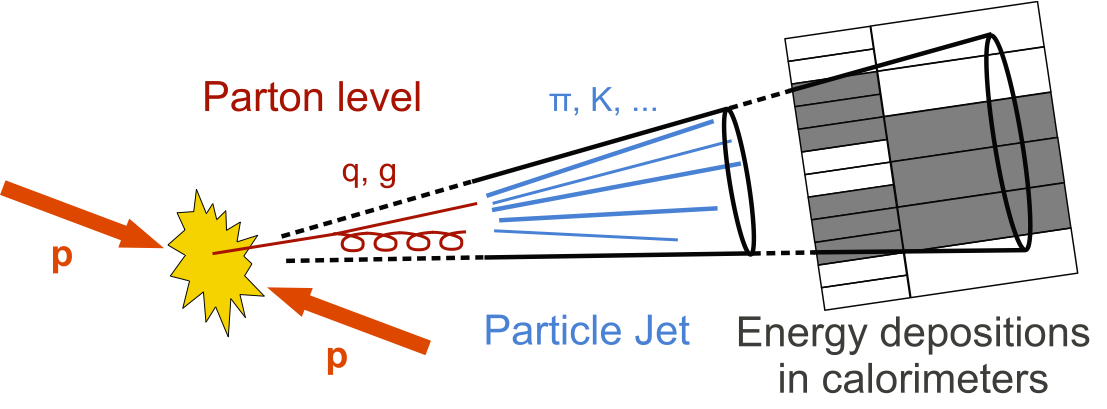
\includegraphics[width=12cm]{physics_objects_plots/Jet1}
\end{figure}

Jets are obvious structures when one looks at an event display, and by measuring their energy and direction one can get close to the idea of the original parton (Fig. \ref{jet2figure}).
\begin{figure}[H]
\caption{CMS event display for a dijet reaction \label{jet2figure}}
  \centering
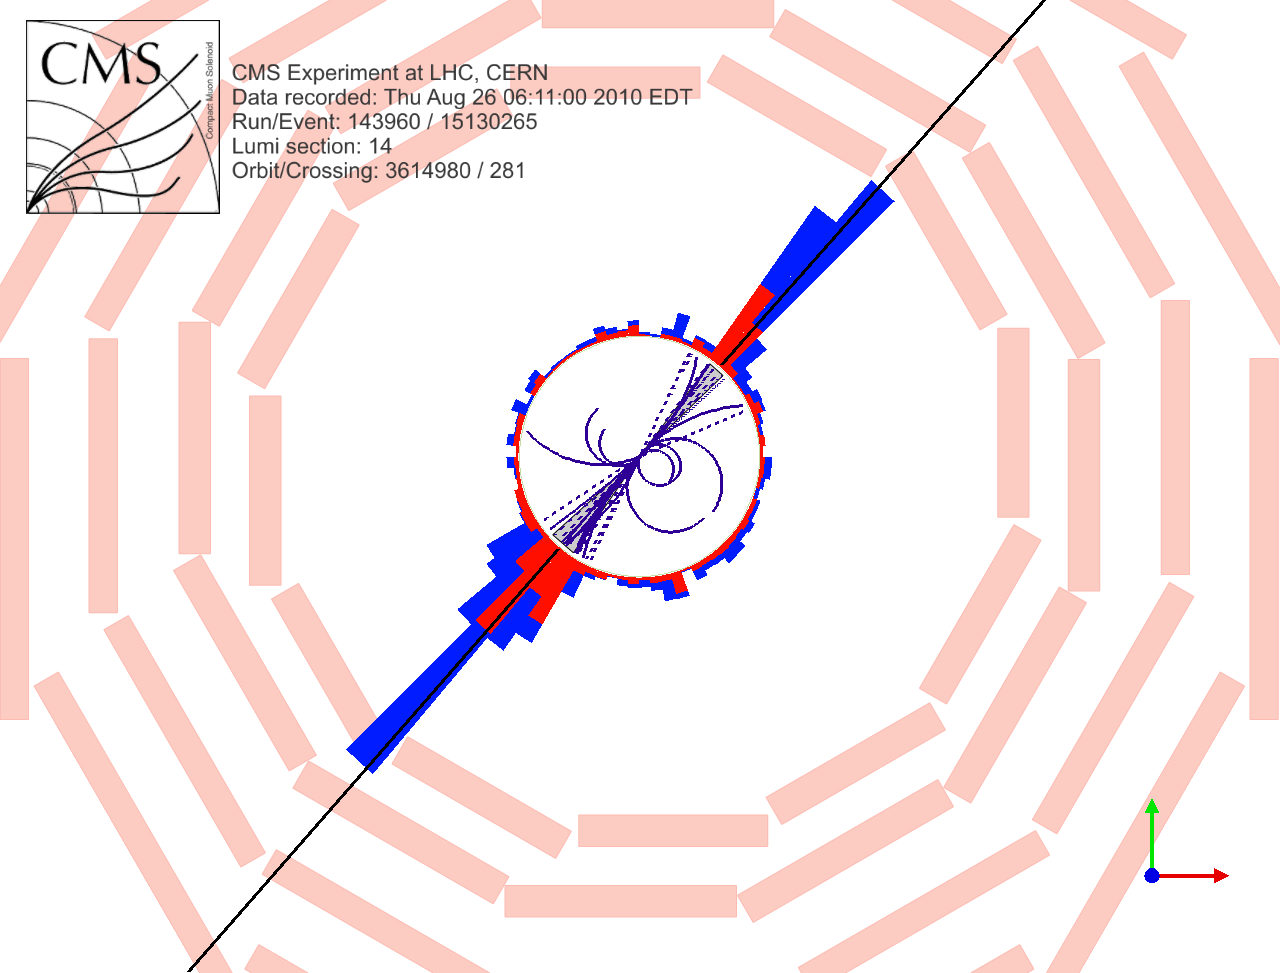
\includegraphics[width=8cm]{physics_objects_plots/Jet2}
\end{figure}

Jet clustering algorithms provide a set of rules for grouping particles into jets. They usually involve one or more parameters that indicate how close two particles must be for them to belong to the same jet. Additionally they are always associated with a recombination scheme, which indicates what momentum to assign to the combination of two particles. Taken together, a jet algorithm with its parameters and a recombination scheme form a jet definition.
There are many types of jet algorithms in the market, but in run-2 CMS will mainly use the anti-kt algorithm. First we introduces the distances $d_{ij}$ between entities (particles, pseudojets) $i$ and $j$ and $d_{iB}$ between entity $i$ and the beam (B). The (inclusive) clustering proceeds by identifying the smallest of the distances and if it is a $d_{ij}$ recombining entities $i$ and $j$, while if it is $d_{iB}$ calling
$i$ a jet and removing it from the list of entities. The distances are recalculated and the procedure repeated until no entities are left. The definitions:
\begin{eqnarray}
d_{ij} &=& \text{min}\left(k^{2p}_{ti},k^{2p}_{tj} \right) \dfrac{\Delta^{2}_{ij}}{\Delta R^{2}}\\
d_{iB} &=& k^{2p}_{ti}
\end{eqnarray}

where $\Delta^{2}_{ij}= (y_{i}-y_{j})^{2}+(\phi_{i}-\phi_{j})^{2}$ and $k_{ti}$, $y_{i}$, $\phi_{i}$ are respectively the transverse momentum, the rapidity and the azimuth of particle $i$. $\Delta R$ is the geometrical distance $\Delta R=\sqrt{\Delta\eta^{2} + \Delta\phi^{2}}$. Note that when $p=-1$ we are on the case of  the anti-kt algorithm, which is implemented in the FastJet package.


\subsection{Particle Flow Jet (PFJet)}

The Particle-Flow (PF) jets are reconstructed by clustering the four-momentum vectors of particle-flow candidates. The particle-flow algorithm combines the information from all
relevant CMS sub-detectors to identify and reconstruct all visible particles in the event, namely muons, electrons, photons, charged hadrons, and neutral hadrons. The energy of charged hadrons is determined from a combination of the track momentum and the corresponding ECAL and HCAL energy, corrected for zero-suppression effects, and calibrated for the non-linear response of the calorimeters. The energy of neutral hadrons is obtained from the corresponding calibrated ECAL and HCAL energy. The PF jet momentum and spatial resolutions are greatly improved with respect to calorimeter jets, as the use of the tracking detectors and of the high granularity of ECAL allows resolution and measurement of charged hadrons and photons inside a jet, which together constitute $\sim$ 85$\%$ of the jet energy.

\subsubsection{Charged hadron subtraction (CHS)}

Contamination to the jet from pileup degrades the ability to reconstruct the jet observables. Previous pile up corections applied in Run I help to correct the four-vector of the jet but not
the jet structure observables. One new approach is use tracking information which takes advantage of the fact that a large fraction of the pileup vertices are separated in space from the vertex of interest. Therefore, charged particles from pileup vertices can be removed from the jets, in a process called "charged hadron subtraction" (CHS) (Fig. \ref{jetchsfigure}). Charged Hadron Subtraction (CHS) is a technique used to reduce the effect of "in-time pileup" on reconstructed physics objects. In this approach, charged hadrons unambiguously associated
to pileup vertices are removed from the event and the remaining PF candidates are allowed to cluster to form jets.
\begin{figure}[H]
  \centering
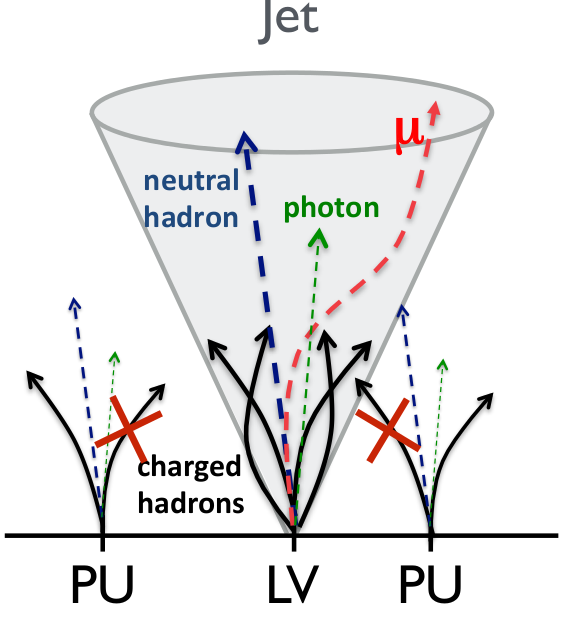
\includegraphics[width=6cm]{physics_objects_plots/chs}
\caption{Charged hadron subtraction. \label{jetchsfigure}}
\end{figure}

\subsection{Jet Energy Correction ( JEC)}\label{jec}

Jet energy corrections need to be applied to account for the non-linear and non-uniform response of the CMS calorimeters. They associate, on average, the $\ptrans$ of a reconstructed jet to the $\ptrans$ of the corresponding particle jet. Jet energy measured in the detector is typically different from the corresponding particle jet energy. The latter is obtained in the simulation by clustering, with the same jet algorithm, the
stable particles produced during the hadronization process that follows the hard interaction. The main cause for this energy mismatch is the non-uniform and non-linear response of the CMS calorimeters. Furthermore, electronics noise and additional pp interactions in the same bunch crossing (event pile-up) can lead to extra unwanted energy. The purpose of the jet energy correction is to relate, on average, the energy measured in the detector to the energy of the corresponding particle jet.

CMS uses a factorized multi-level jet correction, shown schematically in Fig. \ref{jet3figure}, in
which the correction must be applied in the following fixed sequence:
\begin{enumerate}
\item 
\textbf{L1:Offset}: Required correction for pile-up and electronic noise.
\item
\textbf{L2:Relative} ($\eta$): Required correction for variations in jet response with pseudorapidity relative to a control region.
\item
\textbf{L3:Absolute} ($p_{T}$): Required correction to particle level versus jet pT in the control region.
\item
\textbf{EMF}: Optional correction for variations in jet response with electromagnetic energy fraction.
\item
\textbf{Flavor}: Optional correction to particle level for different types of jets (light quark, c, b, gluon).
\item
\textbf{Underlying Event}: Optional correction for underlying event energy due to soft interactions involving spectator partons.
\item
\textbf{Parton}: Optional correction to parton level.
\end{enumerate}
\begin{figure}[H]
\caption{Schematic picture of the factorized multi-level jet correction. \label{jet3figure}}
  \centering
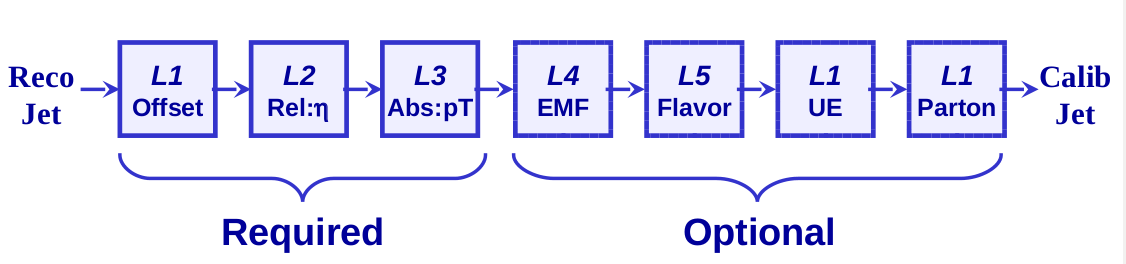
\includegraphics[width=13cm]{physics_objects_plots/jetcorr2}
\end{figure}
Factorization facilitates the use of data-driven corrections, breaking the correction into pieces that are naturally measured in collider data. Combined correction brings back the jet to the particle level.

\begin{comment}
\subsection{Jets identifiction}\label{jetid}

CMS has developed jet quality criteria (“Jet ID”) for PF jets which
are found to retain the vast majority of real jets in the simulation while rejecting most fake
jets arising from calorimeter and/or readout electronics noise. These are studied in pure noise
non-collision data samples such as cosmic trigger data or data from triggers on empty bunches
during LHC operation.

The PF jets are required to have charged hadron fraction CHF $>$ 0.0 if within tracking fiducial region of $\left| \eta \right| <$ 2.4, neutral hadron fraction NHF $<$ 1.0, charged electromagnetic (electron) fraction CEF $<$ 1.0, and neutral electromagnetic (photon) fraction NEF $<$ 1.0. These requirements remove fake jets arising from
spurious energy depositions in a single sub-detector. Jets in the presented studies are required
to pass Jet ID criteria.

The PFJetID efficiency was estimated using the tag-and-probe technique in real and simulated
dijet events. According to this technique one of the two jets, chosen randomly, is the probe jet
and it has to satisfy always the PFJetID criteria. The other one is the probe jet. The efficiency
is then the ratio of all probe jets passing the PFJetID criteria over all the probe jets. In the $\left| \eta \right|$  region 0-2.5 and 3-5 the efficiency of tight PFJetID for both
data and MC is close to 100$\%$, meaning that the PFJetID did not remove real physics jets, since
the selected sample is clean of noise. For the $\left| \eta \right| $ bin 2.5-3.0, the efficiency drops to $\sim$ 91 and $\sim$ 96 for real and simulated jets respectively.


\subsection{Pileup subtraction using jet areas}
\end{comment}


\subsection{V-tagging}

Generally, V tagging methods (V=Z,W weak vector boson) have depended largely on leptonic decay channels. Hadronic signatures deal with the relatively poorer reconstruction of jets and large multijet backgrounds from QCD processes at hadron colliders. Several recent developments have improved the tagging of hadronically decaying weak vector bosons. Many of these advances have resulted from the analysis of the internal components
of a jet, i.e. its substructure.

A more effective identification of hadronic V decays allows many analyses to profit from the substantially larger branching fraction of hadronic channels. This, in turn, may provide significant gains in searches for new physics.

\subsubsection{Unresolved jets}

For highly boosted weak vector bosons, the hadronic decay products can be merged into a single jet. For distance parameter R = 0.8, this occurs for boson pT above 200 GeV. The radiation profile of the individual, hard partons within a merged jet must be explicitly resolved for an accurate calculation of the boson mass. This contrasts with the resolved scenario, for which the boson mass can be determined simply from the properties of the individually reconstructed jets. A new class of observables has been developed for disentangling the radiation profiles of proximate partons. We explore these observables in this section.

Jet mass is the most natural discriminator between jets originating from V decays and those originating from single partons. Jet grooming techniques improve mass resolution by reducing the effects from pileup and underlying event. The following grooming algorithms are studied:

\paragraph{N-subjetiness}\label{tau21sec}
This method uses the distribution of jet constituents relative to the jet axis in order to quantify how well the jet can be divided into N subjets. The computation is done by reclustering the jet using the kT-algorithm until N protojets are left. The direction of the remaining jets are then used to compute the "N-subjetiness" as
\begin{eqnarray}
\tau_{N}=\dfrac{1}{d_{0}} \sum_{k}\: p_{T,k}\times \text{min}\left( \Delta R_{1,k}, \Delta R_{2,k},\dots,\Delta R_{N,k}\right) 
\end{eqnarray}
with the normalization factor $d_{0}$ :
\begin{eqnarray}
d_{0} = \sum_{k} p_{T,k}\times R_{0}
\end{eqnarray}
and $R_{0}$ is the clustering parameter of the original jet, $p_{ T,k}$ is the pT of the k-th jet constituent and $\Delta R_{n,k}$ is its distance to the n-th subjet. In particular, the ratio of the "2-subjettiness" to the "1-subjettiness" $(\tau_{2} / \tau_{1} = \tau_{21} )$ has excellent capability at separating jets originating from boosted vector bosons from jets originating from quarks and gluons.
\begin{figure}[H]
\caption{$\tau_{21}$ distribution for signal and background \label{jettau21figure}}
  \centering
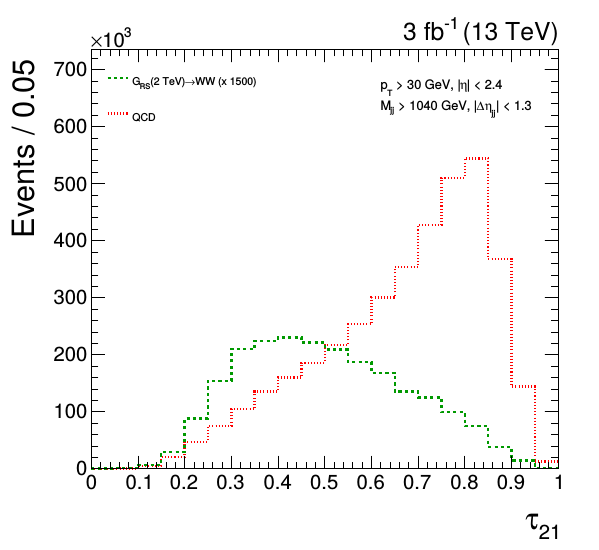
\includegraphics[width=8cm]{physics_objects_plots/tau21}
\end{figure}

\paragraph{Pruning}\label{prun}
This method attempts to isolate subjet showers by removing soft, large angle particles from each subjet. Pruning will remove the uncorrelated contributions from underlaying events and pile up that make significant contributions to the jet mass. The mass of the resulting pruned jet is small if we start with a QCD jet, and near the particle mass if we start with a jet containing the decay products of a heavy particle. 
%Procedure: Define parameters $z_{\text{cut}}$=0.1 and $r_{\text{cut}}=0.5$. Reclustering with sequential recombination algorithm (CA), veto soft and large-angle recombination between pseudojets $i$ and $j$:
\begin{eqnarray}
\Delta R_{ij}> r_{\text{cut}}\times\dfrac{2m}{p_{T}},\ \ \  \ \  z=\text{min}\left( \dfrac{p_{Ti}, p_{T_{j}}}{p_{T_{i+j}}} \right) < z_{\text{cut}}  
\end{eqnarray}

\begin{figure}[H]
\caption{Pruned mass distribution for signal and background \label{jetprunfigure}}
  \centering
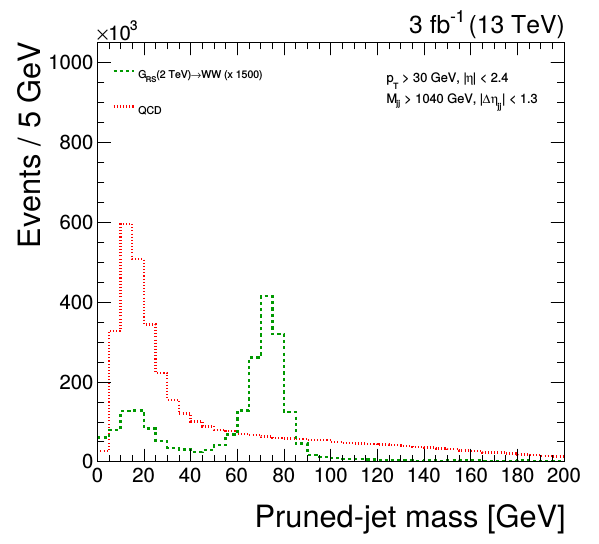
\includegraphics[width=8cm]{physics_objects_plots/prun}
\end{figure}

\begin{comment}
\subsection{b-jets}
\end{comment}

\section{Missing Transverse Energy ($\met$) }\label{MET1}

Missing transverse momentum plays a critical role in many physics analyses at the LHC. It is a key variable in many searches for physics beyond the standard model, such as extra dimensions and supersymmetry as well as for collider dark matter searches. Some neutral particles which interact weakly with matter ( \ie   neutrinos ) leave the detector without producing any direct response in the detector components. The presence of such particles (also called invisible particles, Fig. \ref{figuremet1}) must be implied from the imbalance of total momentum considering that the detector is hermetic. The vector momentum imbalance in the plane perpendicular to the beam direction is particularly useful in $\cPp\cPp$ and $\ppbar$ colliders, and is known as missing transverse momentum, here denoted $\vec{\met}$ . Its magnitude is called missing transverse energy, and is denoted $\met$ (MET).

\begin{figure}[H]
\caption{Invisible and visible particles \label{figuremet1}}
  \centering
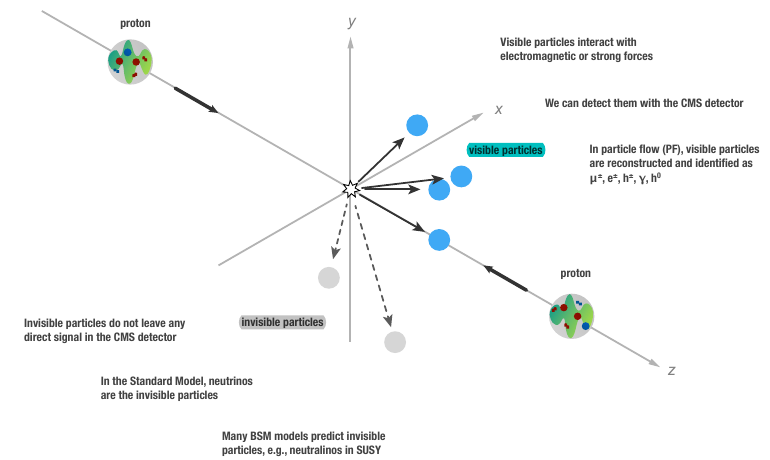
\includegraphics[width=14cm]{physics_objects_plots/met_rec}
\end{figure}

In general $\vec{\met}$ is calculated as the negative of the vector sum of the components of momentum transverse to the beam axis of all final-state particles reconstructed in the detector. CMS has developed three distinct algorithms to reconstruct $\vec{\met}$. (a) Calo $\met$  based on calorimeter energies and calorimeter tower geometry, (b) TC $\met$ calculated by replacing the calorimeter tower energies matched to charged hadrons with their corresponding charged-track momenta, and (c)PF $\met$ calculated using a complete particle-flow technique. In thi work we will focus on PF $\met$.

The $\met$ reconstruction is sensitive to detector malfunctions and various reconstruction effects resulting in particle momentum mismeasurements and particle misidentification. Precise calibration of all physics objects is crucial for the $\met$ reconstruction, and $\met$ is particularly sensitive to multiple proton-proton interactions in the same, earlier, and later bunch crossings (pileup interactions). Thus, it is essential to study reconstruction in detail with data.

In Run-I, identifying and removing the causes of large fake $\met$ was the major challenge in $\met$ reconstruction at CMS. By the time Run-I ended in early 2013, it was developed a matured set of $\met$ filters to reject such large fake $\met$. These filters are used in the event selections of many physics analyses. Below is a list of the main filters:
\begin{itemize}
\item 
CSC tight beam halo filter
\item
HBHE noise filter with isolated noise rejection
\item
HCAL laser filter
\item
ECAL dead cell trigger primitive (TP) filter
\item
Tracking failure filter
\item
Bad EE Supercrystal filter
\item
ECAL Laser correction filter
\item
Tracking POG filters
\end{itemize}

Some filters are used online in HLT. After the $\met$ filters are applied, the agreement of the $\met$ spectrum
with simulation, significantly improves (Fig. \ref{figuremetmiss} )
\begin{figure}[H]
\caption{Comparison before and after apply the $\met$ Filters. \label{figuremetmiss}}
  \centering
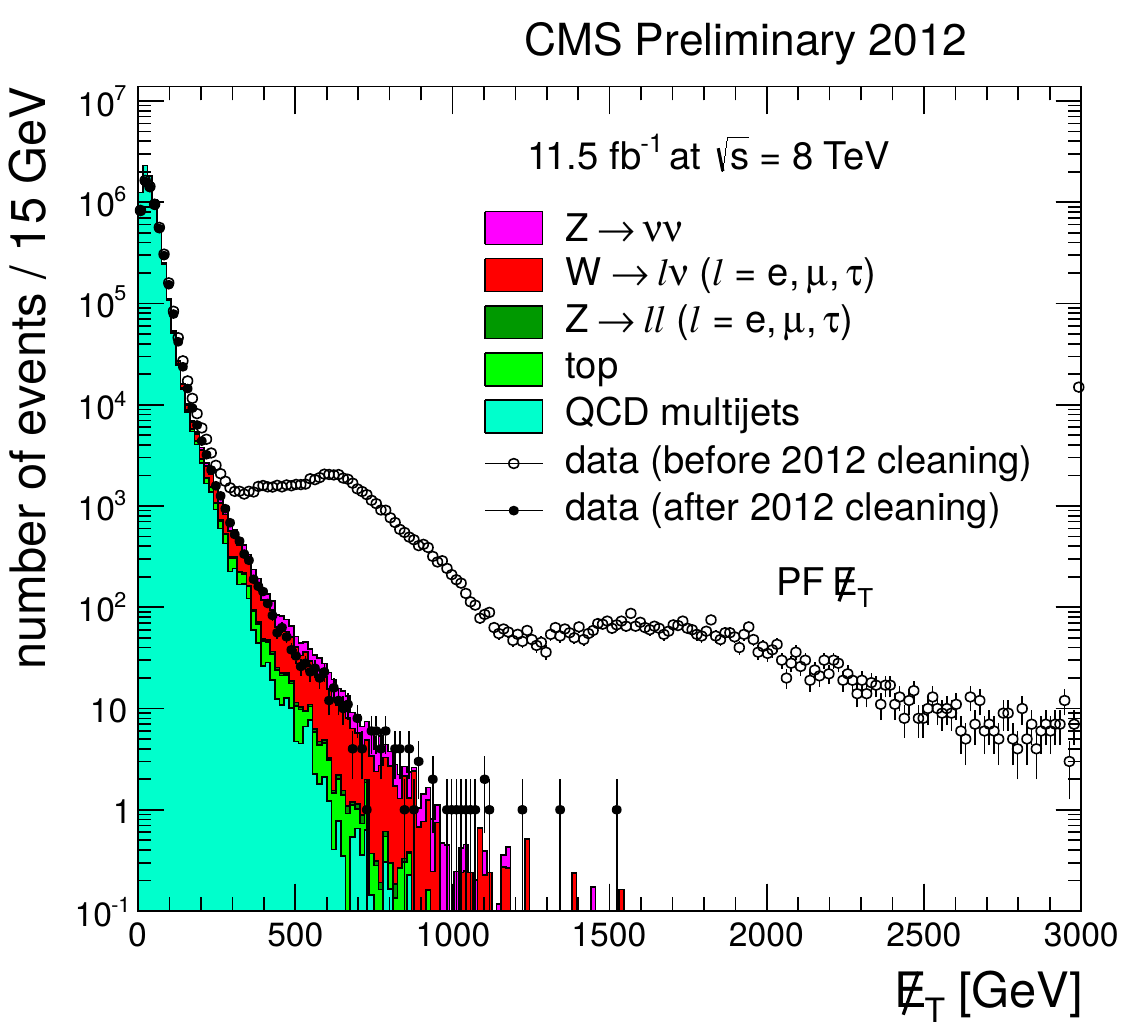
\includegraphics[width=8cm]{physics_objects_plots/met_missrec}
\end{figure}

\subsection{Particle Flow MET (PF $\met$)}

The particle flow technique aims to reconstruct a complete, unique list of particles in each event using an optimal combination of information across all CMS subdetector systems. Particles which are
reconstructed and identified include muons, electrons (with associated bremsstrahlung photons), photons (unconverted and converted), and charged and neutral hadrons. The PF $\met$ hereafter called MET is then simply the negative vector sum of all such reconstructed particles in the event (Fig. \ref{figuremet2}).
\begin{eqnarray}
\vec{\met} = - \sum_{i \in  \text{vis.}}\:\vec{p}_{\mathrm{T}_{i}} 
\end{eqnarray}

\begin{figure}[H]
\caption{Vector sum of the reconstructed particles in the event. \label{figuremet2}}
  \centering
\includegraphics[width=14cm]{physics_objects_plots/met2}
\end{figure}

\subsection{The Type-I Correction}\label{typeI}

Raw MET is the negative of the vector sum of all reconstructed particles. The raw MET is systematically different from true MET, i.e., the transverse momentum carried by invisible particles, for many reasons including the non-compensating nature of the calorimeters and detector misalignment. To make MET a better estimate of true MET, MET corrections can be applied. The Type-I correction is the most popular MET correction in CMS. This correction is a propagation of the jet energy corrections (JEC) to MET. The Type-I correction replaces the vector sum of transverse momenta of particles which can be clustered as jets with the vector sum of the transverse momenta of the jets to which JEC is applied. 
\begin{eqnarray}
\vec{\met}^{\text{raw}} = - \sum_{i\in \text{all}}\:\vec{p}_{\,\mathrm{T}_{i}} 
\end{eqnarray}

The particles can be classified into two disjoint sets: either clustered as jets or unclustered
\begin{eqnarray}
\vec{\met}^{\text{raw}} = - \sum_{i\in \text{jets}}\:\vec{p}_{\,\mathrm{T}_{i}} - \sum_{i\in \text{uncl.}}\:\vec{p}_{\,\mathrm{T}_{i}}
\end{eqnarray}

The vector sum of $\ptrans$ of all particles clustered as jets is the same as the vector sum of $\ptrans$ of all jets.
\begin{eqnarray}
\sum_{i\in\text{jets}}\:\vec{p}^{\,\text{raw}}_{\,\mathrm{T}_{\text{jet}}} = \sum_{i\in \text{jets}}\:\vec{p}_{\,\mathrm{T}_{i}} 
\end{eqnarray}
\begin{eqnarray}
\vec{\met}^{\text{raw}} = - \sum_{\text{jet}}\:\vec{p}^{\,\text{raw}}_{\,\mathrm{T}_{\text{jet}}} - \sum_{i\in \text{uncl.}}\:\vec{p}_{\,\mathrm{T}_{i}}
\end{eqnarray}

The Type-I correction replaces the raw jet pT with the corrected jet pT
\begin{eqnarray}
\vec{C}^{\text{Type-I}}_{T}= \sum_{\text{jet}}\:\vec{p}^{\,\text{raw}}_{\,\mathrm{T}_{\text{jet}}} - \sum_{\text{jet}}\:\vec{p}^{\,\text{JEC}}_{\,\mathrm{T}_{\text{jet}}}
\end{eqnarray}

The Type-I correction is a vector term that can be added to raw MET
\begin{eqnarray}
\vec{\met}^{\text{Type-I}} = \vec{\met}^{\text{raw}} + \vec{C}^{\text{Type-I}}_{T}
\end{eqnarray}
The Type-I corrected MET can be written as
\begin{eqnarray}
\vec{\met}^{\text{Type-I}} =  - \sum_{\text{jet}}\:\vec{p}^{\,\text{JEC}}_{\,\mathrm{T}_{\text{jet}}} - \sum_{i\in \text{uncl.}}\:\vec{p}_{\,\mathrm{T}_{i}
\end{eqnarray}


\subsection{Transverse Mass}\label{transvserve}

In this analysis we perform a search in the JET + MET final state as we will discuss in detail in the next chapter. The strategy is search for an excess related with the mass of the resonance. For that reason is neccesary introduce a variable associated with this magnitude. Since the invisible particles are not directly detected in the experiment, it is difficult to reconstruct the mass of the resonance. Consider a single heavy particle of mass $M$ which decays in a JET (labeled particle 1) and MET (labeled particle 2). The mass of the parent particle can be constrained with the quantity $M_{T}$ defined by:
\begin{eqnarray}
M_{T}^{2} &=& (E_{T}(1)+E_{T}(2))^{2}  - (\vec{p}_{T}(1)+\vec{p}_{T}(2))^{2}\nonumber\\
&=& E_{T}(1)^{2} + E_{T}(2)^{2} +2 E_{T}(1)E_{T}(2) -\vec{p}_{T}(1)^{2} - \vec{p}_{T}(2)^{2} -2\vec{p}_{T}(1)\cdot \vec{p}_{T}(2)\nonumber\\
\end{eqnarray}
Considering that:
\begin{eqnarray}
E_{T}^{2} = m^{2}+\vec{p}_{T}^{2},\ \   \text{and}\ \  m(1),m(2) \approx 0
\end{eqnarray}
We obtain:
\begin{eqnarray}
M_{T}^{2} = 2 \left| \vec{p}_{T}(1)\right| \left| \vec{p}_{T}(2)\right| \left(1-\cos\phi \right) 
\end{eqnarray}
Remember that: $p_{T}(1)=p_{T}^{\text{jet}},\ \   \text{and}\ \  \met=p_{T}(2)$.
Finally we get:
\begin{eqnarray}
M_{T} = \sqrt{\:2\: p_{T}^{\text{jet}}\: \met\: \left[ 1-\cos\Delta\phi\left( \text{jet}, \met\right)  \right] } 
\end{eqnarray}


\begin{comment}
\section{Muons}\label{muons}

The muon reconstruction is done prior to the particle-flow event reconstruction. The recon-
structed muons [12], referred to as “reco muons” in the following, contain a significant amount
of misidentified (un-decayed) charged hadrons. In order to have a pure sample of muon can-
didates, identification requirements must be applied to the original reco muon collection. A
standard choice of possible selections is presented in Ref. [12] and will be referred as soft,
global and tight muon selections, hereafter. The particle-flow algorithm makes use of some of
these identification tools and together with the use of the measurement of energy released in
the calorimeter, defines an alternative set of selections which are appropriate for and needed
by the particle-flow algorithm.


In the standard CMS reconstruction for pp collisions [2, 15], tracks are first reconstructed independently in the inner tracker (called \emph{tracker track)} and in the muon system ( called \emph{standalone-muon track}).
Based on these objects, two reconstruction approaches are used:

Global Muon reconstruction (outside-in). For each standalone-muon track, a matching
tracker track is found by comparing parameters of the two tracks propagated onto a
common surface. A global-muon track is fitted combining hits from the tracker track
and standalone-muon track, using the Kalman-filter technique. At large trans-
verse momenta, p T 200 GeV/c, the global-muon fit can improve the momentum
resolution compared to the tracker-only fit.

Tracker Muon reconstruction (inside-out). In this approach, all tracker tracks with p T >
0.5 GeV/c and total momentum p > 2.5 GeV/c are considered as possible muon can-
didates and are extrapolated to the muon system taking into account the magnetic
field, the average expected energy losses, and multiple Coulomb scattering in the
detector material. If at least one muon segment (i.e., a short track stub made of DT
or CSC hits) matches the extrapolated track, the corresponding tracker track qualifies as a Tracker Muon. Track-to-segment matching is performed in a local (chamber)
coordinate system, where local x is the best-measured coordinate (in the $r-\varphi$ plane)
and local y is the coordinate orthogonal to it. The extrapolated track and the seg-
ment are considered to be matched if the distance between them in local x is less
than 3 cm or if the value of the pull for local x is less than 4, where the pull is defined



\subsection{Muon isolation} 
The requirement that a muon is an isolated particle in the event, meaning that the energy flow
in its vicinity is below a certain threshold, can effectively discriminate muons from the decays
of W and Z bosons from those produced in heavy-flavor decays and hadron decays in flight.
The discriminating variable $I_{\text{rel}}$ (RelIso) is the sum of the $\pt$ of all charged hadrons, the transverse energies $\ET$ of all photons, and $\ET$ of all neutral hadrons reconstructed by the PF algorithm within a cone of radius $\Delta R <$ 0.4 centred on the muon track direction, divided by the muon track $\pt$:

\begin{eqnarray}
I_{\text{rel}} = \dfrac{\sum \pt(\text{charged}) + \max \left[\sum \ET (\text{neutral}) + \sum \ET (\text{photon})-\Delta \beta, 0 \right]  }{\pt}
\end{eqnarray}

here $\Delta \beta$ is a correction based on the $\sum \pt$ of the charged particles in the cone of interest but with particles not originating from the primary vertex (PU corrections).

\begin{figure}[H]
\caption{Schematic illustration of the isolation cone. The muon direction at the vertex
defines the cone axis. The energy deposit in the cone is computed, and the muon contribution is removed by excluding the small area around the muon (the veto value) from the cone. Comparison of the deposit in the cone with a predefined threshold determines the muon isolation. \label{muoniso}}
  \centering
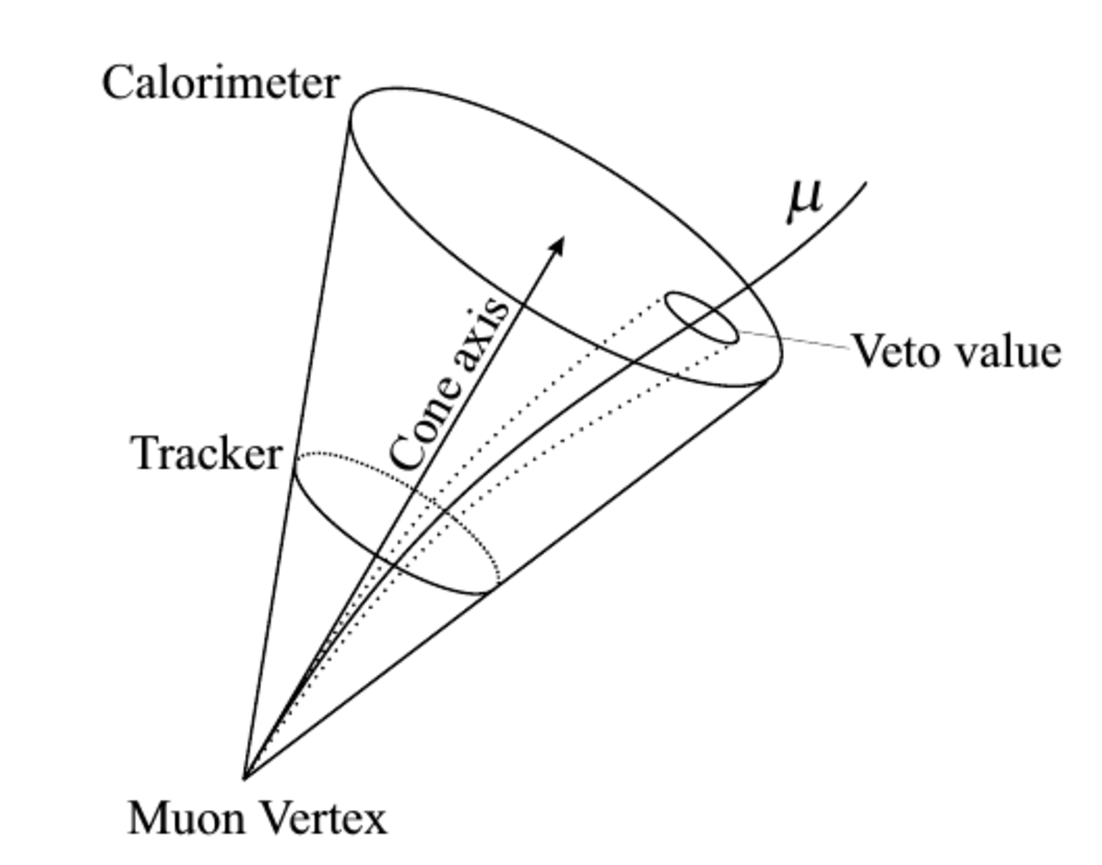
\includegraphics[width=10cm]{Chapter3_plots/muoniso.pdf}
\caption*{Source: Technical design report, CERN-LHCC-2006-001, CMS-TDR-008-1.}
\end{figure}

  
\section{Electrons }\label{electrons}

\section{Photons }\label{photons}

\section{Taus }\label{taus}
\end{comment}

\chapter{Data Samples and Monte Carlo Simulation}\label{samples}

\section{Trigger and data samples}

\par The data employed for this search were collected by the CMS experiment at $\sqrt{s} = 13$ TeV, and correspond to a total integrated luminosity of 2.3 {\fbinv}.
Signal event candidates are recorded online using a trigger designed to select $\HT^{\text{miss}}$ and $\MET$ with a lower threshold of 90 GeV in each case.
The $\HT^{\text{miss}}$ is computed as the magnitude of a vectorial sum of the transverse momenta of all jets with  $\pt$ greater than 20 GeV.
To reject events arising from atypical detector performance, supplementary selection requirements are set on the jets used in the $\HT^{\text{miss}}$ calculation.
The $\MET$ is defined as the magnitude of the negative vectorial sum of the transverse momentum of all the particles identified at the trigger level.
Identified muons are removed from the event before the $\MET$ and $\HT^{\text{miss}}$ are calculated.
And additional support trigger was used in combination with the main signal trigger. This trigger select events that contains $\MET$ with a lower threshold of 170 GeV. Selected events are required to have $\MET >$ 250 GeV to guarantee a trigger efficiency greater than 98$\%$ for all events used in the analysis. The trigger paths are reported in the Table \ref{tab:triggerPaths}. For additional information about the trigger paths and the efficiency calculation, we refer the reader to the Appendix \ref{appendix:ApendiceA}.

\begin{table}[!ht]
\footnotesize
\begin{center}
\caption{HLT Trigger path with their respective criteria.}
\label{tab:triggerPaths}
\begin{tabular}{cc} \hline
Trigger path & Criteria  \\ \hline
\verb|PFMETNoMu90_JetIdCleaned_PFMHTNoMu90_IDTight| (unprescaled)  &  $\MET>$ 90 GeV, $H_{\text{T}}^{\text{miss}}>$ 90 GeV\\
\verb|PFMET170_*| (unprescaled)  &  $\MET>$ 170 GeV \\ \hline
\end{tabular}
\end{center}
\end{table}

We use about 2.3 fb$^{-1}$ of data collected during the Run2015C and Run2015D era (Table \ref{tab:datasamples}) and reconstructed with the CMSSW 7 6 X release. We employ only lumisections that have been declared good for analysis by the central certification team.

\begin{table}[!ht]
\begin{center}
\caption{Data samples.}
\label{tab:datasamples}
\begin{tabular}{cc} \hline
Sample & Number of events  \\ \hline
\verb|MET/Run2015D| & 17996789   \\
\verb|MET/Run2015C| & 106269  \\ \hline
\end{tabular}
\end{center}
\end{table}


\section{Simulated Samples}

The analysis makes use of various simulated event samples for modeling the SM background and signal processes. A benchmark model, the bulk graviton (spin-2), is used to illustrate typical signal behavior. Simulated signal samples of bulk graviton resonances decaying to dibosons (ZZ) and subsequently to quarks and neutrinos are generated at leading order (LO) with the $\MADGRAPH 5$ \cite{Alwall:2014hca}  program interfaced with $\PYTHIA$8 \cite{Sjostrand:2006za,Sjostrand:2007gs} for the parton showering and hadronization, considering a coupling constant $\tilde{k}$ = 0.5. For this model we considered defined values of the resonances mass in the range 0.8 $ \leq m_{X} \leq $ 2 TeV in steps of 100 GeV. We restrict the analysis to scenarios where the natural width of the resonance is sufficiently small to be neglected when compared to the detector resolution. This makes our modelling of the detector effects on the signal shape independent of the actual model used for generating the events. The signal samples used in the analysis are shown in Table \ref{tab:signalsamples}.

\par Simulated samples are produced for the Z+jets, W+jets, $t\bar{t}$, dibosons and QCD multijet processes in order to describe the contribution expected from SM backgrounds. The main components of the total background are represented by Z + jets ($Z \rightarrow \nu \bar{\nu}$) and W+ jets ($W \rightarrow \ell \nu$) production. These as well as the QCD multijets sample, are simulated with $\MADGRAPH 5$ in LO mode and matched to $\PYTHIA$8 using the CUETP8M1 tune for hadronization and fragmentation. Double counting by the matrix element calculation and parton showering is resolved by using the MLM matching prescription \cite{Mangano:2002ea}. The SM background contribution from $t\bar{t}$ events is modeled at next-to-leading order (NLO) with the $a\MCATNLO$ program \cite{Frixione:2002ik}, interfaced with $\PYTHIA$8. Inclusive non-resonant dibosons simulated samples (WW/WZ/ZZ) are generated at LO with $\PYTHIA$8. All the background samples used in this analysis are listed in Table \ref{tab:backgroundsamples}.

\par The V+jets simulated samples are rescaled using next-to-next-to-leading order (NNLO) QCD correction in the cross sections (Table \ref{tab:scalefactors}) and NLO QCD electroweak (EW) correction in the V boson $\pt$ domain (Fig. \ref{fig:EW}) \cite{Kallweit:2015dum}. 

\par Minimum bias events are included during the production of the simulated samples to account for contributions from additional proton-proton collisions (pileup) with the number of reconstructed primary vertices matching those in data. The simulation is corrected from perceptible differences between data and simulation in the trigger and identification/isolation efficiency of leptons (electrons, muons, taus), photons and jets originating from hadronization of bottom quarks (b-jets).

\par In all the simulated samples, the events are generated using the NNPDF 3.0~\cite{Ball:2011mu} set of parton distribution functions. The simulation of the detector response is modeled with the \GEANTfour package~\cite{Agostinelli:2002hh}.

\begin{table}[!ht]
\footnotesize
\begin{center}
\caption{Monte Carlo simulated signal samples for Bulk graviton model.}
\label{tab:signalsamples}
\begin{tabular}{lcc} \hline
Sample & Cross Section (pb) & $\text{N}_{\text{events}}$ \\ \hline
\verb|BulkGravToZZToZhadZinv_narrow_M-800_13TeV-madgraph| & 1.0 & 100000 \\
\verb|BulkGravToZZToZhadZinv_narrow_M-1000_13TeV-madgraph| & 1.0 & 99200 \\
\verb|BulkGravToZZToZhadZinv_narrow_M-1200_13TeV-madgraph| & 1.0 & 95800 \\
\verb|BulkGravToZZToZhadZinv_narrow_M-1400_13TeV-madgraph| & 1.0 & 100000 \\
\verb|BulkGravToZZToZhadZinv_narrow_M-1600_13TeV-madgraph| & 1.0 & 100000 \\
\verb|BulkGravToZZToZhadZinv_narrow_M-1800_13TeV-madgraph| & 1.0 & 98000 \\
\verb|BulkGravToZZToZhadZinv_narrow_M-2000_13TeV-madgraph| & 1.0 & 99200 \\
\verb|BulkGravToZZToZhadZinv_narrow_M-2500_13TeV-madgraph| & 1.0 & 99200 \\
\verb|BulkGravToZZToZhadZinv_narrow_M-3000_13TeV-madgraph| & 1.0 & 99600 \\
\verb|BulkGravToZZToZhadZinv_narrow_M-3500_13TeV-madgraph| & 1.0 & 100000 \\
\verb|BulkGravToZZToZhadZinv_narrow_M-4000_13TeV-madgraph| & 1.0 & 99200 \\
\verb|BulkGravToZZToZhadZinv_narrow_M-4500_13TeV-madgraph| & 1.0 & 99000 \\ \hline
\end{tabular}
\end{center}
\end{table}


\begin{table}[!ht]
\small
\begin{center}
\caption{Monte Carlo background samples.}
\label{tab:backgroundsamples}
\begin{tabular}{lcc} \hline
Sample & Cross Section (pb) & $\text{N}_{\text{events}}$ \\ \hline
$Z(\rightarrow \nu \bar{\nu})$+jets, $100 < \HT < 200$ GeV & 280.35 & 5240199 \\
$Z(\rightarrow \nu \bar{\nu})$+jets, $200 < \HT < 400$ GeV & 77.67 & 5135542 \\
$Z(\rightarrow \nu \bar{\nu})$+jets, $400 < \HT < 600$ GeV  & 10.73 & 954435  \\
$Z(\rightarrow \nu \bar{\nu})$+jets, $\HT > 600$ GeV & 4.116 & 1033818 \\ \hline
$W(\rightarrow \ell \nu)$+jets, $100 < \HT < 200$ GeV & 1345 & 10205377  \\
$W(\rightarrow \ell \nu)$+jets, $200 < \HT < 400$ GeV & 359.7  & 4949568  \\
$W(\rightarrow \ell \nu)$+jets, $400 < \HT < 600$ GeV & 48.91 & 1943664  \\
$W(\rightarrow \ell \nu)$+jets, $\HT > 600$ GeV & 18.77 & 1041358  \\ \hline
QCD multjets,$100 < \HT < 200$ GeV & 27990000  & 82095800 \\
QCD multjets,$200 < \HT < 300$ GeV & 1712000 & 18784379 \\
QCD multjets,$300 < \HT < 500$ GeV & 347700 & 16909004  \\
QCD multjets,$500 < \HT < 700$ GeV & 32100  & 19665695  \\
QCD multjets,$700 < \HT < 1000$ GeV& 6831  & 15547962 \\
QCD multjets,$1000 < \HT < 1500$ GeV & 1207 & 5049267 \\
QCD multjets,$1500 < \HT < 2000$ GeV & 119.9 & 3939077  \\
QCD multjets,$ \HT > 2000$ GeV & 25.24 & 1981228 \\ \hline
$t\bar{t}$ & 831.76 & 38475776 \\ 
$t\bar{t}$ (Extension) & 831.76 & 196937036 \\ \hline
$WW$ & 118.7 & 988418 \\
$WZ$ & 47.13  & 985600    \\
$ZZ$ & 16.523 & 996944 \\ \hline
\end{tabular}
\end{center}
\end{table}

\begin{table}[!ht]
\begin{center}
\caption{NNLO QCD flat scale factors.}
\label{tab:scalefactors}
\begin{tabular}{lc} \hline
Sample & Scale factor \\ \hline
Z + jets &  1.23   \\
W + jets  &  1.21\\ \hline
\end{tabular}
\end{center}
\end{table}

\begin{figure}[!ht]
\begin{center}
  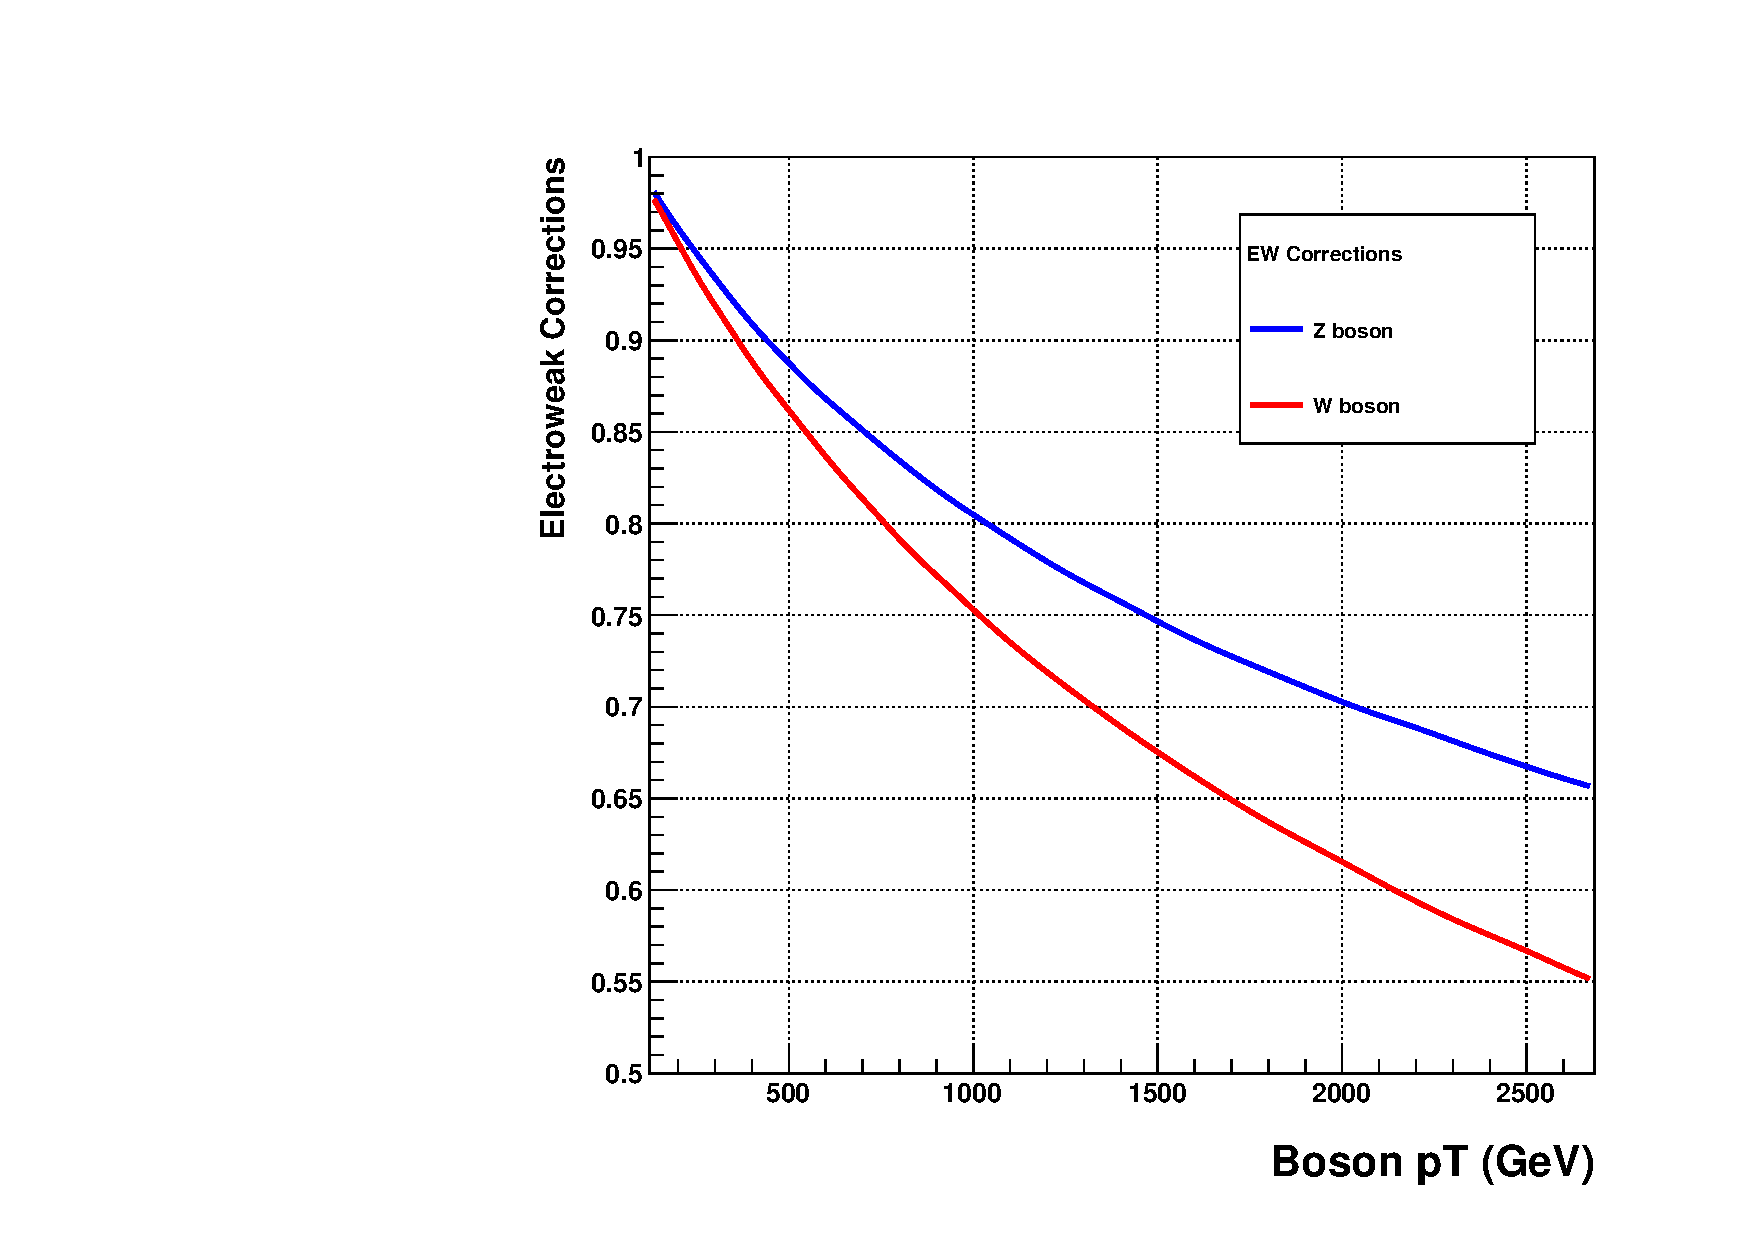
\includegraphics[width=240pt]{figures/Samples/EWcorrections.pdf}
\end{center}


\caption{Electroweak corrections for the W/Z boson in function of the boson $\pt$.}
\label{fig:EW}
\end{figure}



\chapter{Object Reconstruction and Identification}\label{obj_reco_id}

\section{Primary Vertices}

In general, many primary vertices are reconstructed in an event beacuse of the pileup contributions. In order to identify the vertex related with the main proton-proton collision in the analized event,  we required that:

\begin{itemize}
\item
Number of degrees of freedom:  $n_{\text{dof}} >$ 4
\item
longitudinal coordinate: $z_{0} <$ 24 mm
\item
Transverse position: $d_{0}<$ 2 mm 
\item
Vertex fit variable: $\chi^{2} \neq$ 0
\end{itemize}

If more than one vertex pass the previous conditions, we choose the one with the highest sum of transverse momenta $\sum \pt^{2}$ of the \emph{tracks} associated to it. 
Due to disagreements in the number of primary vertices distribution  between the MC samples and data a reweight procedure was implemented assuming a total inelastic cross section of $\sigma = 69 000 \mu$b. Figure \ref{fig:nv} (Left) shows the comparison for the PU in data and MC (Right) the distribution of the number of primary vertices after apply the reweight procedure. 

\begin{figure}[!ht]
\caption{Left: Comparison between the PU profile in data (blue) and the Poisson density function in MC (green). Right: Number of primary vertices distribution after the reweight procedure in events that pass the final analysis selection.}
\begin{tabular}{cc}
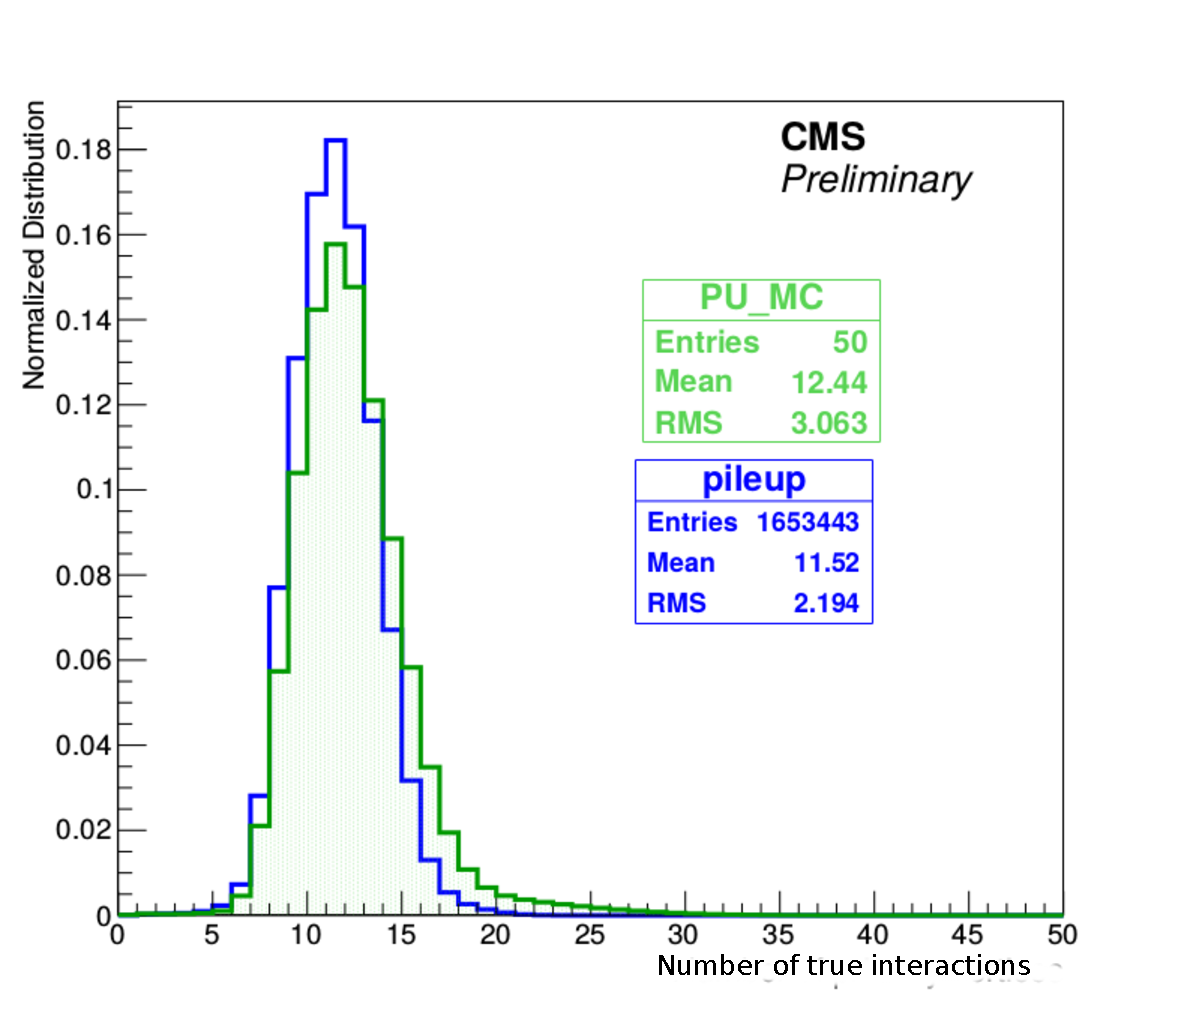
\includegraphics[width=250pt]{figures/Objects/PV.pdf}&
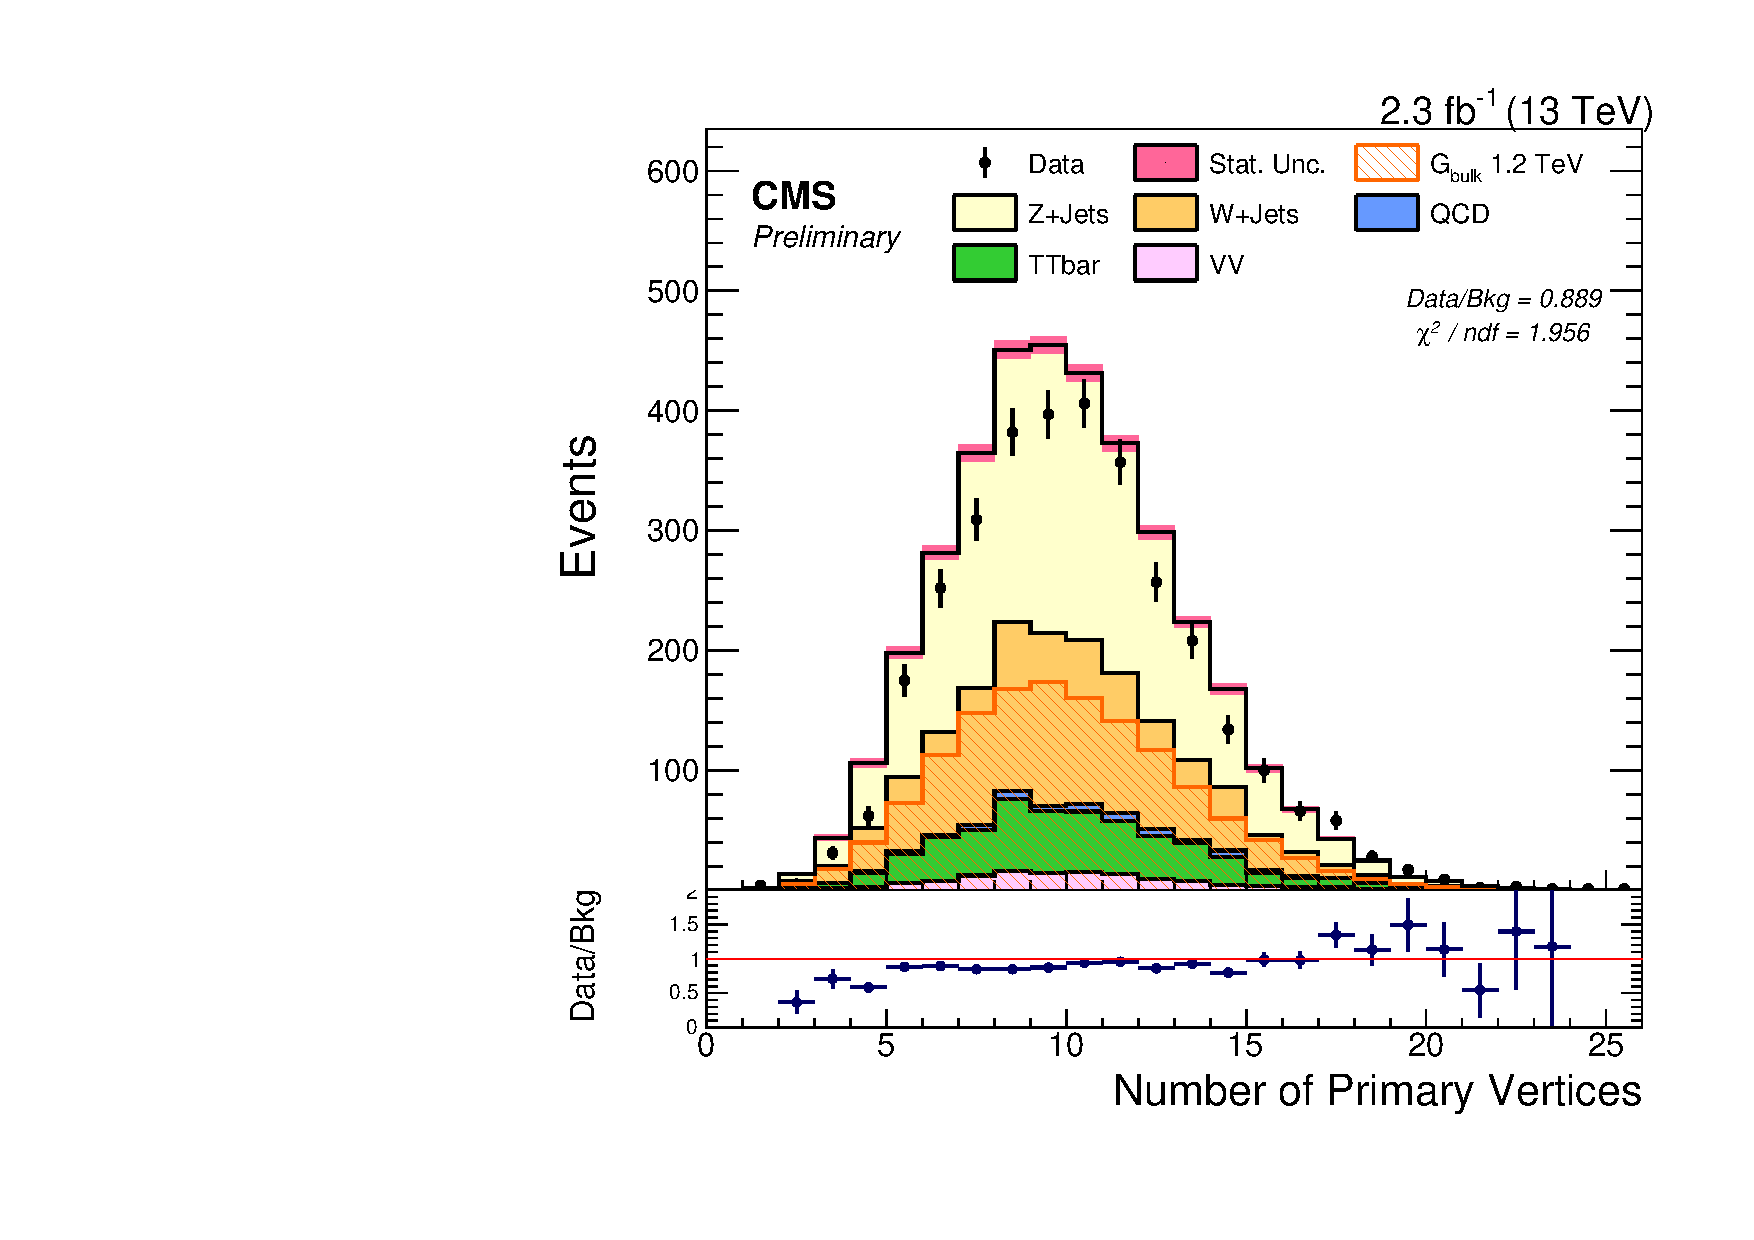
\includegraphics[width=210pt]{figuresARC/CONTROLPLOTS/can_h_nVtx.pdf}\\
\end{tabular}
\label{fig:nv}
\end{figure}

\section{Missing Transverse Energy}\label{met}

The raw missing transverse energy vector is computed as the negative vector sum of the transverse momenta of all particles reconstructed in the event, with magnitude denoted by $\MET$. Corrections to the momenta of jets reconstructed in the event are further propagated to the $\MET$ (Type-1 corrections) \cite{CMS:2016ljj}. Figure \ref{fig:MET} show a comparison between the raw PF $\MET$ and the Type-1 PF $\MET$.

\begin{figure}[!ht]
\caption{Comparison between Raw PF $\MET$ and Type-1 PF $\MET$ corresponding to a signal sample of 1 TeV.}
\begin{center}
  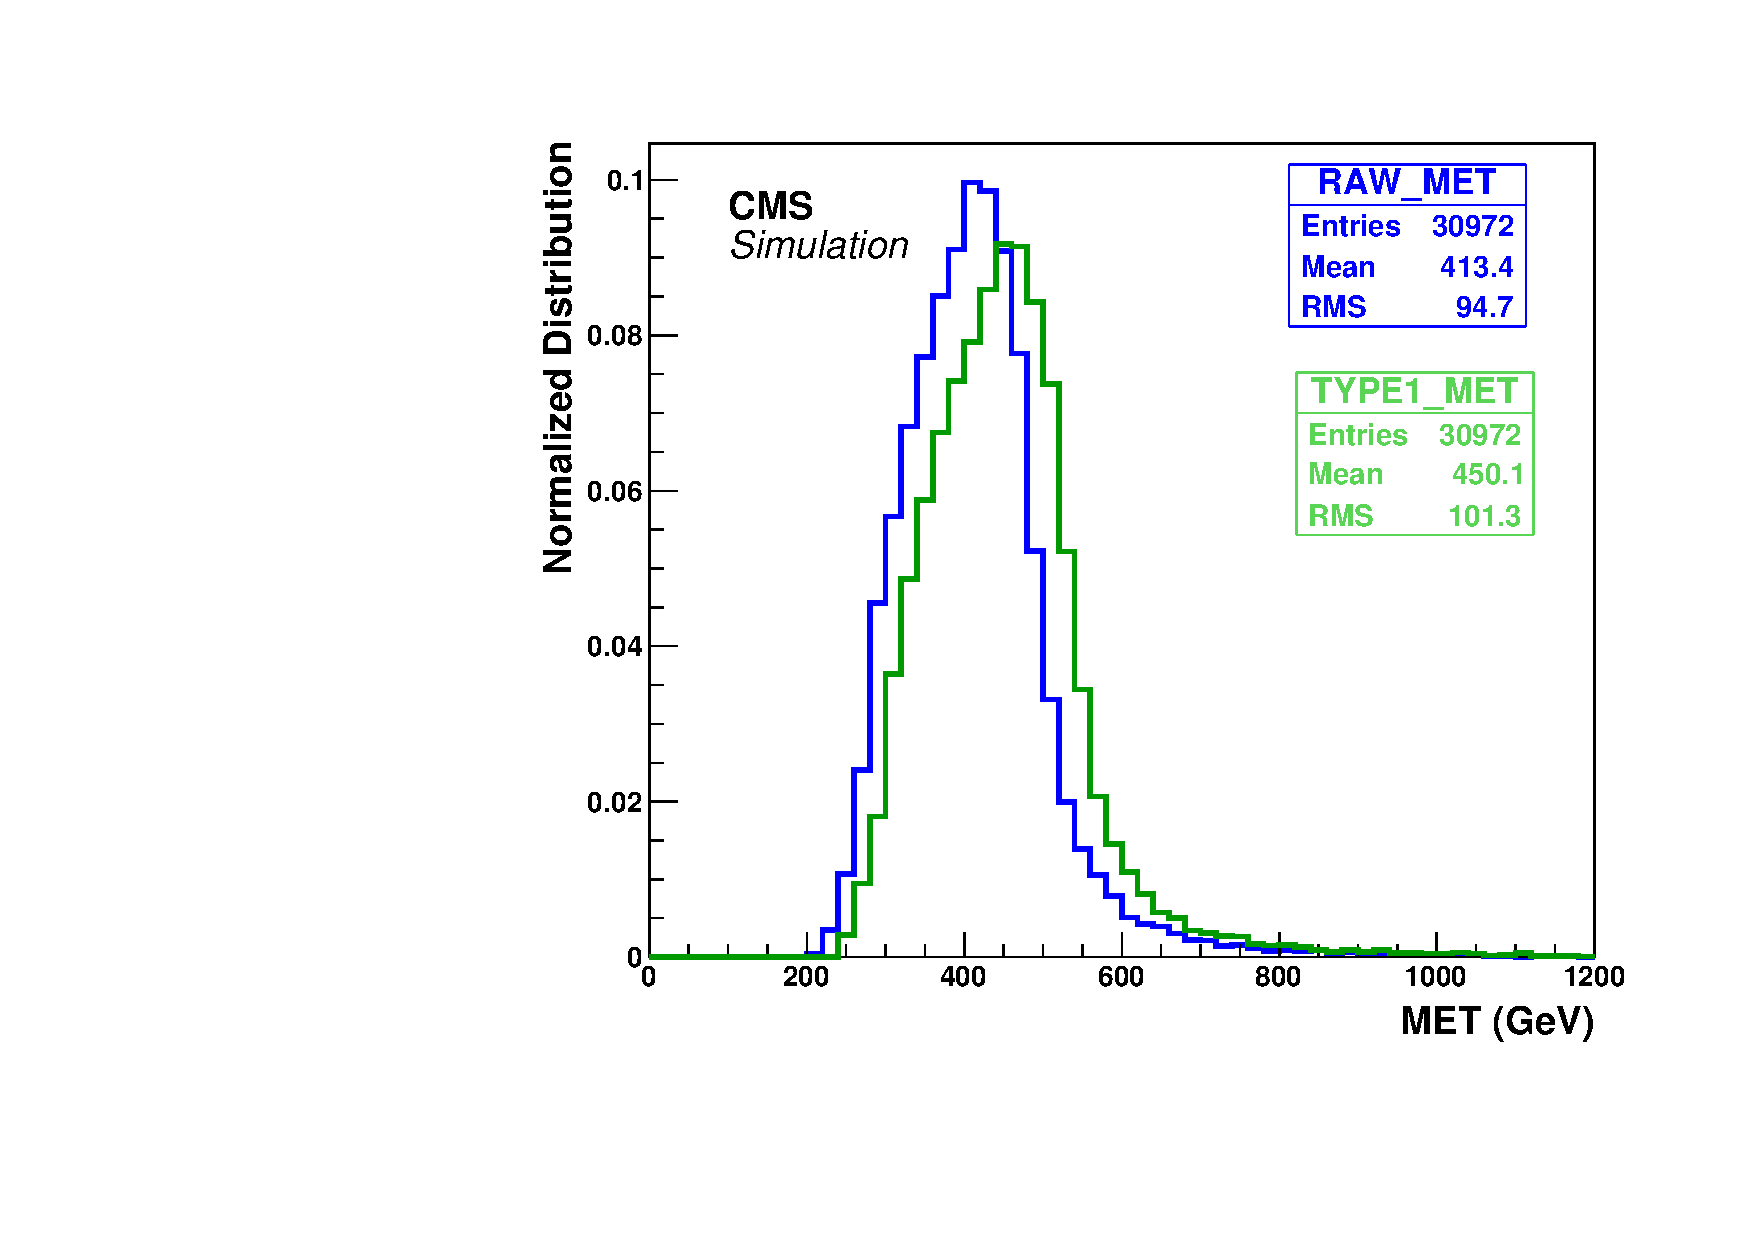
\includegraphics[width=280pt]{figures/Objects/metcomparison.pdf}
\end{center}
\label{fig:MET}
\end{figure}

A set of dedicated quality filters are applied in data and simulation to remove events with a large misreconstructed $\MET$ originated from detector noise and beam backgrounds \cite{CMS:2016ljj}:

\begin{itemize}
\item
HBHENoiseFilter
\item
HBHENoiseIsoFilter
\item
CSCTightHalo2015Filter
\item
EcalDeadCellTriggerPrimitiveFilter
\item
goodVertices
\item
eeBadScFilter
\end{itemize}

\begin{figure}[!ht]
\caption{HBHENoiseFilter efficiency vs AK8 jet $\pt$ in simulation for a signal sample of 1 TeV.}
\begin{center}
  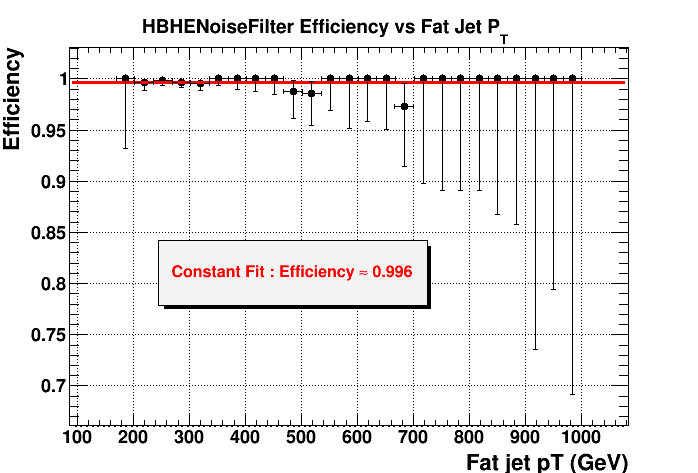
\includegraphics[width=280pt]{Chapter5_plots/effFilter.png}
\end{center}
\label{fig:METfilter}
\end{figure}

Figure \ref{fig:METfilter} shows the efficiency for the events that pass the HBHENoiseFilter for signal sample of 1 TeV. Events containing a minimum $\MET$ of 250 GeV are required in the analysis in order to settle in the plateau of the trigger turn-on curve (Fig. \ref{fig:TriggerEff1}). Further corrections are applied to the $\MET$ in the V+jets simulated samples, based on the hadronic recoil information derived from Z+jets ($Z\rightarrow \ell \ell$)  events in data and simulation (Recoil Correction).

\subsection{Recoil Correction}

We use a data-driven method to model the V boson recoil (response and resolution) in order to improve the description of the missing energy in  V+jets MC events. The term ``recoil'' here means the hadronic activity that balances the $\pt$ of the boson.  To derive the recoil correction we use a Z +jets ($Z \to \mu \mu$ ) process in data and simultion, fitting the response and resolution of the recoil as a function of Z $\pt$. The advantage of using the $Z$+jets process is that the Z boson can be selected without significant background and the $\pt$ can be accurately reconstructed in data from the two final state leptons. The transverse recoil vector is defined as:
\begin{eqnarray}
\vec{u}_{\mathrm{T}} = -\vec{\MET}-\Sigma_{i} \vec{\ell}_{i}
\end{eqnarray}
where $\vec{\ell}_{i}$ is the momentum of the lepton in which the Z decays. Figure \ref{fig:recoil01} shows the kinematics of the process in the transverse plane. The method parametrize the recoil in the parellel and perpendicular directions of the boson $\pt$, fitting these variables with a double gaussian model in different bins of the Z $\pt$. From the fits it can extract the mean an the $\sigma$ of the gaussians, using different polynomial functions to fit these values and extract the response and resolution curves. After this process some scale factors are derived and applied to the  V+jets simulated samples. Complementary information about the recoil method is reported in the Appendix \ref{appendix:ApendiceB}.

\begin{figure}[!ht]
\caption{$Z\rightarrow \ell \ell$ event kinematics in the transverse plane. The transverse recoil vector $\vec{u}_{\mathrm{T}}$ is split into parallel and perpendicular components to the direction of the boson $\pt$. }
\begin{center}
  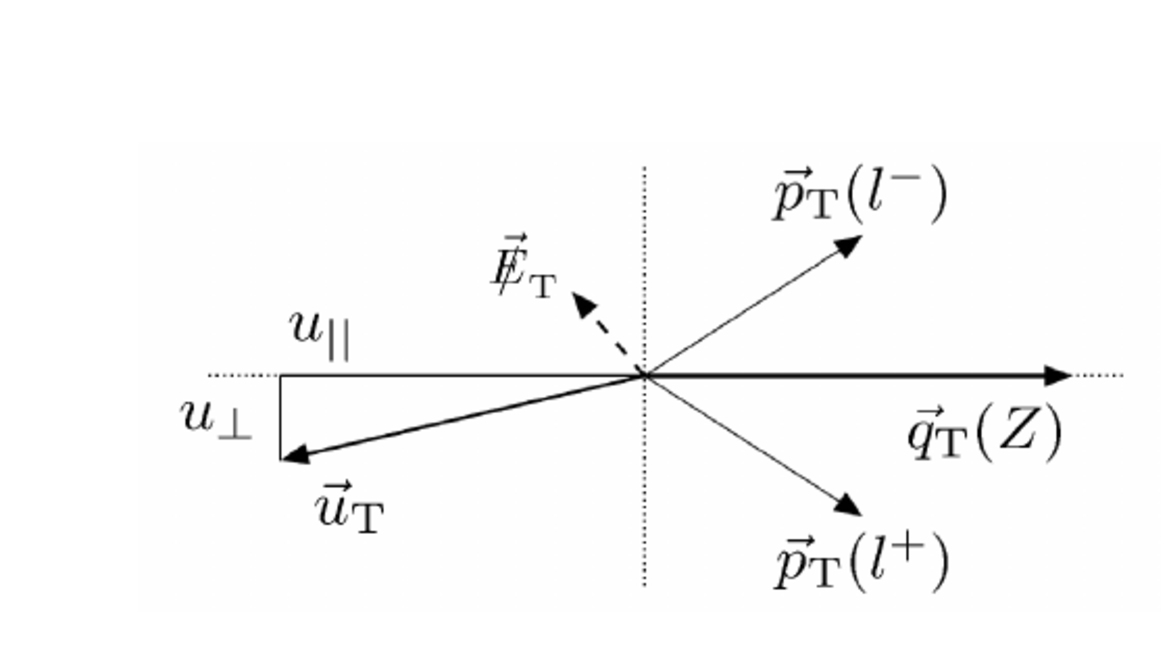
\includegraphics[width=280pt]{Chapter5_plots/recoil.pdf}
\end{center}
\caption*{Source: CMS Collaboration, “Performance of missing energy reconstruction in 13
TeV pp collision data using the CMS detector”, CMS-PAS-JME-16-004, 2016.}
\label{fig:recoil01}
\end{figure}

Figure \ref{fig:METrecoil} shows the transverse missing energy distribution before and after apply the recoil corrections.

\begin{figure}[!ht]
\caption{$\MET$ distribution before and after apply the recoil correction for W +jets and Z + jets samples.}
\begin{tabular}{cc}
  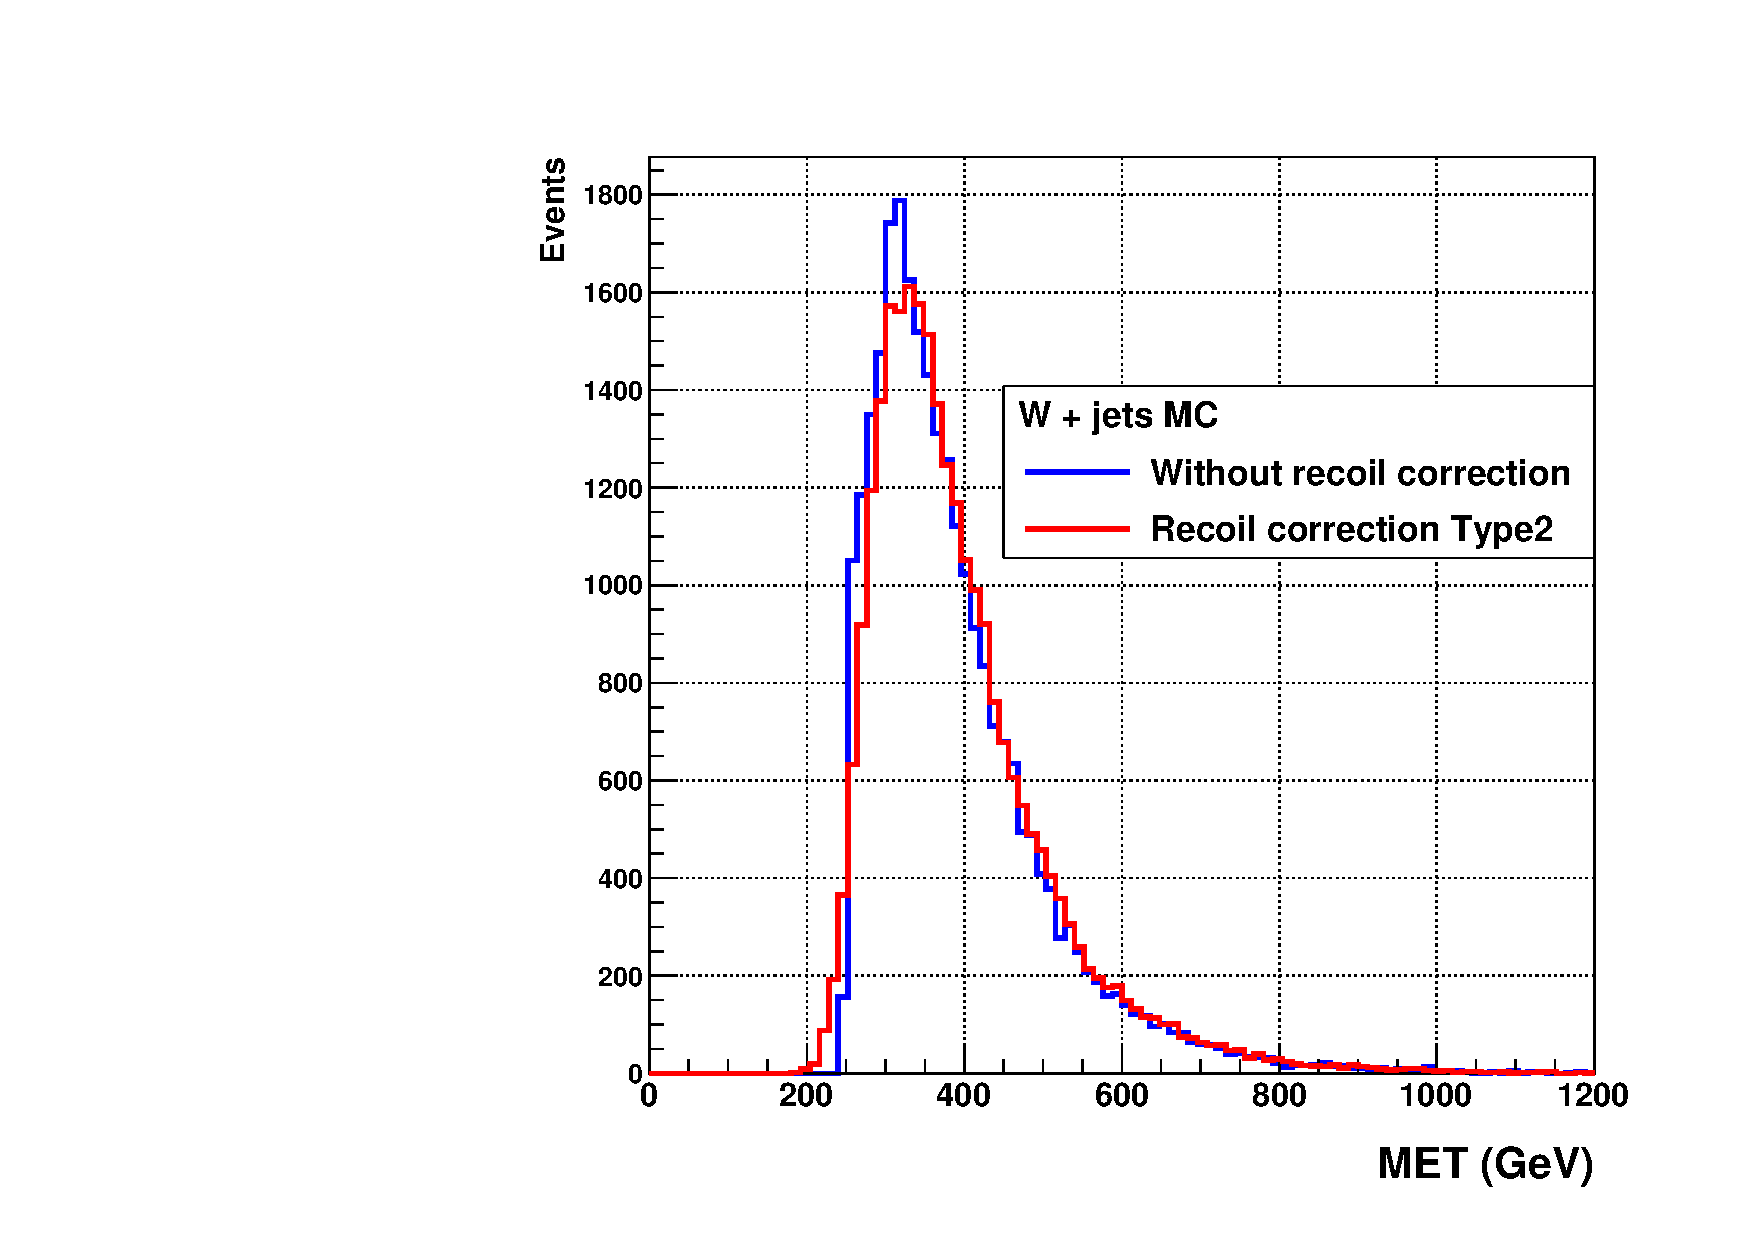
\includegraphics[width=230pt]{figuresARC/recoil/compRecoilCorrWjetsARC.pdf} &
  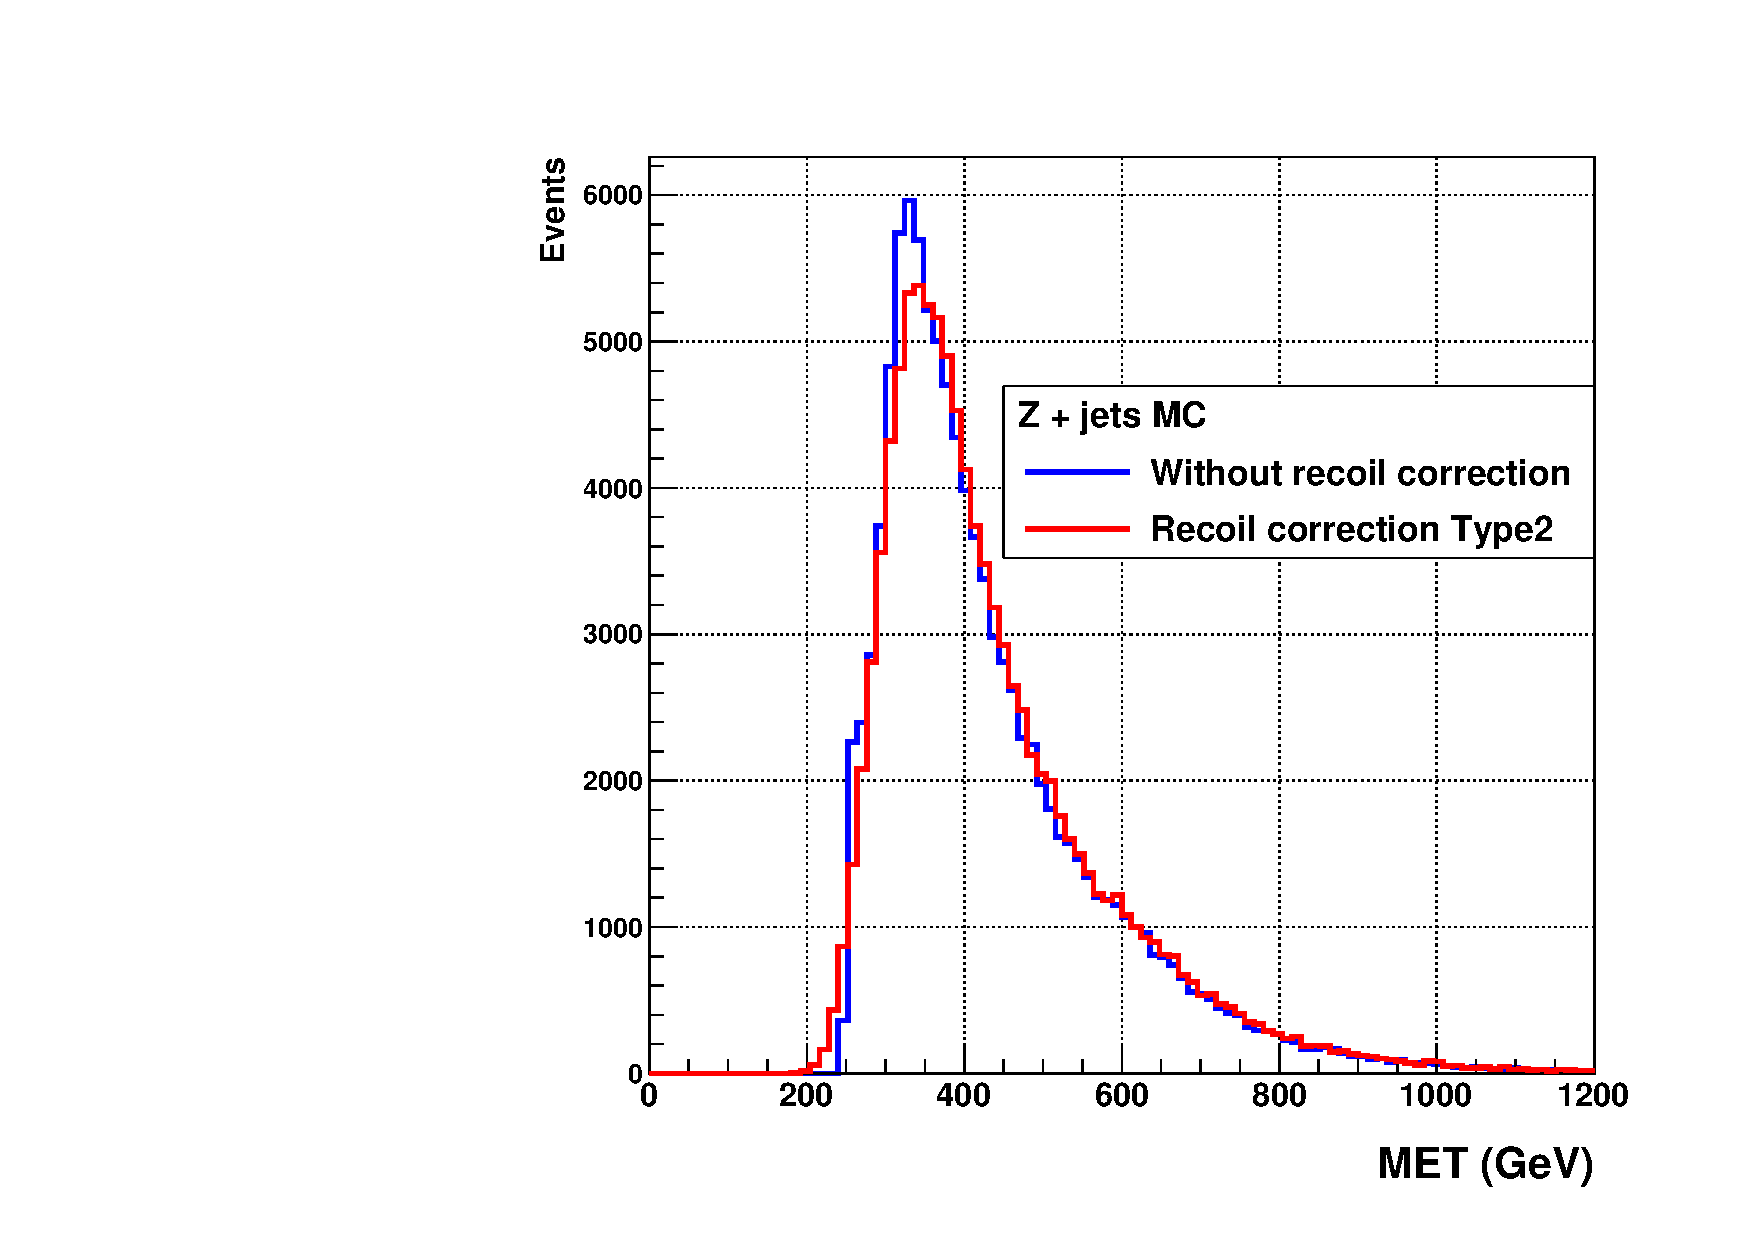
\includegraphics[width=230pt]{figuresARC/recoil/compRecoilCorrZjetsARC.pdf} \\
\end{tabular}
\label{fig:METrecoil}
\end{figure}




\section{Jets}\label{jets}

\par Jets are reconstructed using the PF technique. Charged hadrons not originating from the primary vertex are discarded in a process called ``charged hadron subtraction'' (CHS). The resulting list of particles are used as input to the anti-$\kt$ jet clusterging algorithm with a distance parameter $R$, implemented in the FastJet package. It is applied to the jets a technique based on jet areas that provides jet-by-jet corrections for pileup and underlying-event effects. Jet energies are further corrected using $\pt$ and $\eta$ dependent correction factors. These corrections are derived from MC simulation and are supplemented by residual corrections from dijet and photon+jet events in data. Figure \ref{fig:JEC} shows the comparison of the jet mass distributions before and after apply the JEC.

\begin{figure}[!ht]
\caption{Comparison between corrected and uncorrectd jets (JEC) for the jet mass distribution corresponding to a graviton signal sample  of 1 TeV ($X \rightarrow ZZ$). As it can be observed the corrected distribution shows a peak close to the Z mass (91 GeV).}
\begin{center}
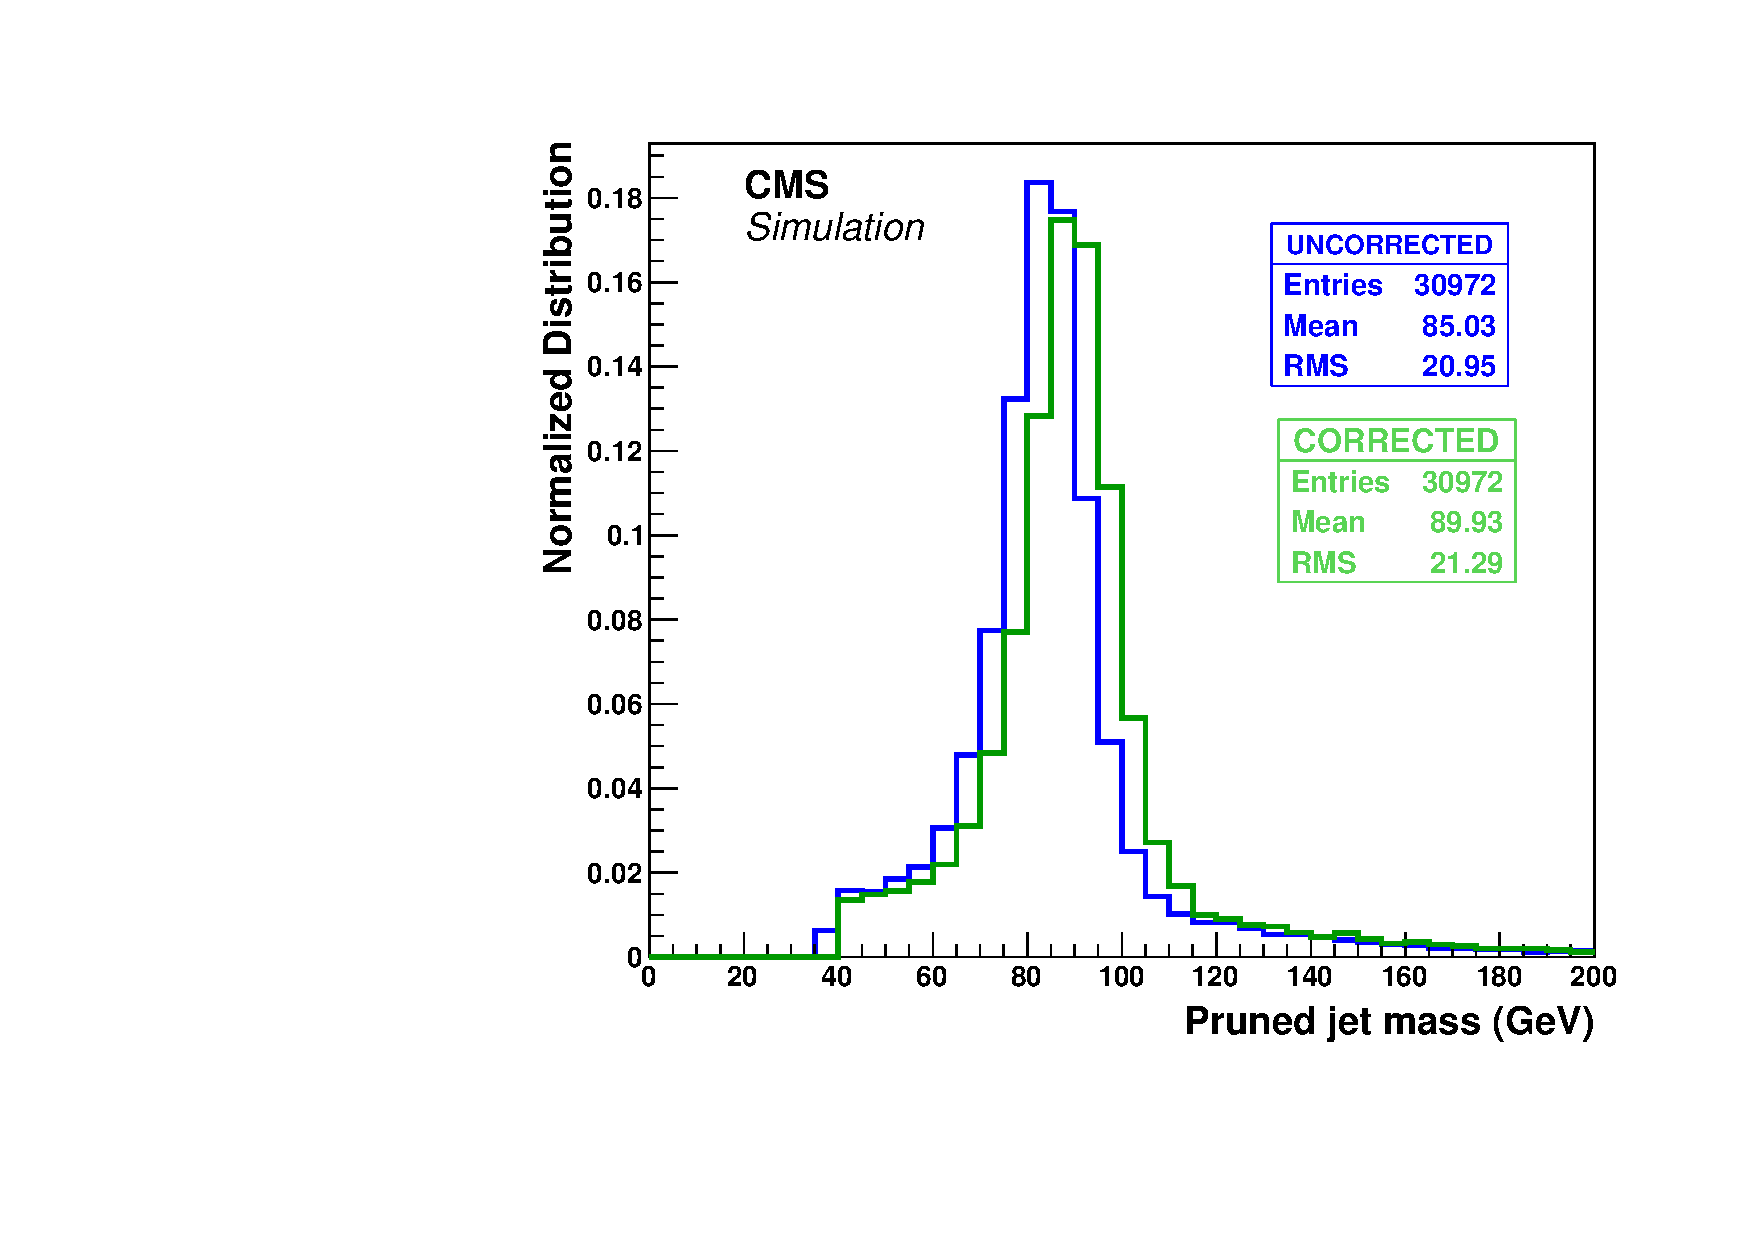
\includegraphics[width=250pt]{figures/Objects/jetcomparison.pdf}     
\end{center}
\label{fig:JEC}
\end{figure}

Loose jet identification criteria are applied to remove spurious jet-like features associated with calorimeter noise. To supress additional instrumental and beam-related backgrounds, events are rejected if less than 10$\%$ of the energy of the highest $\pt$ jet (leading jet) is carried by charged hadrons, or if more than 80$\%$ of this energy is carried by neutral hadrons.
Figure \ref{fig:jetclen} shows the charged hadron fraction (CHF) and neutral hadron fraction (NHF) distributions for events obtained with the full analysis selection after the cleaning cuts were applied. 

\begin{figure}[!ht]
\caption{Jet hadronic energy fractions after the cleaning cuts.}
\begin{tabular}{cc}
  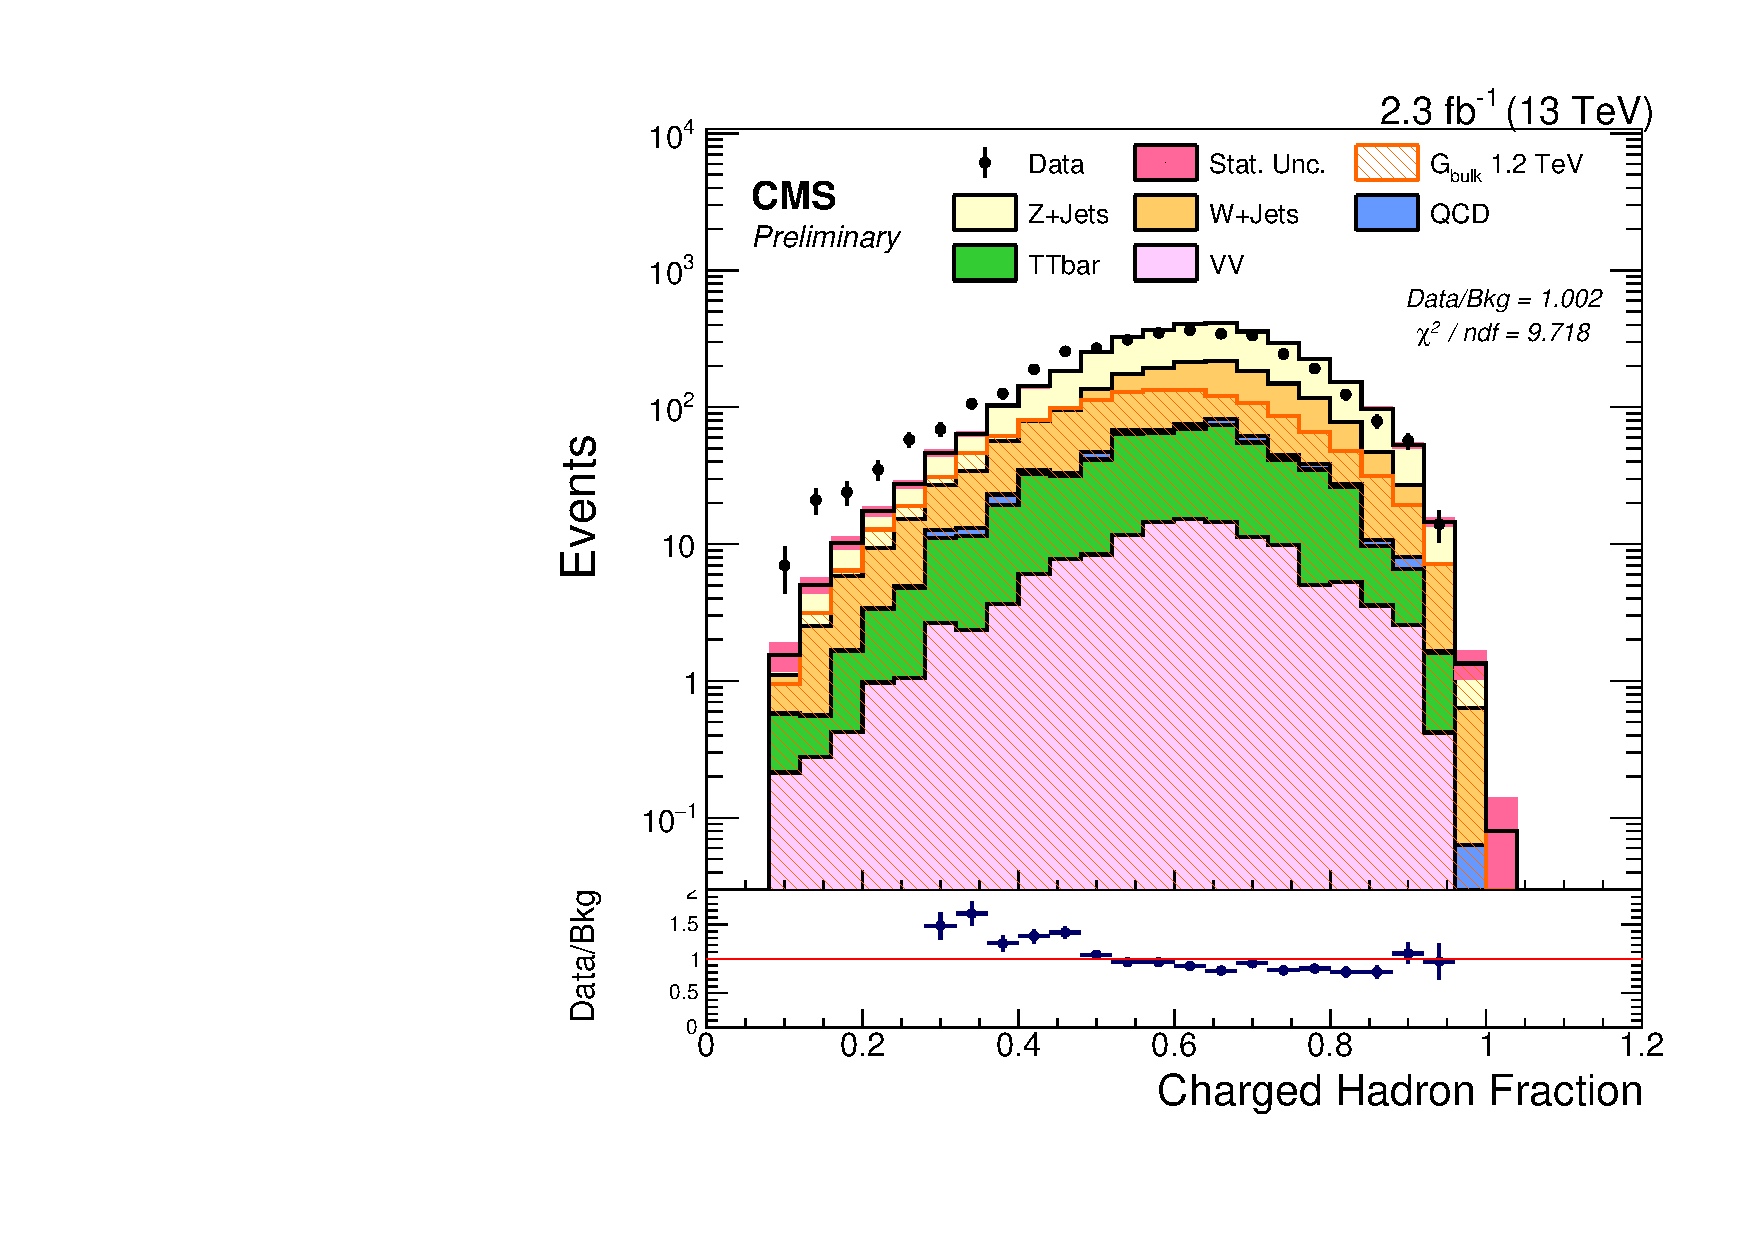
\includegraphics[width=230pt]{figuresCONDI/OBj/LOG_can_h_chf.pdf} &
  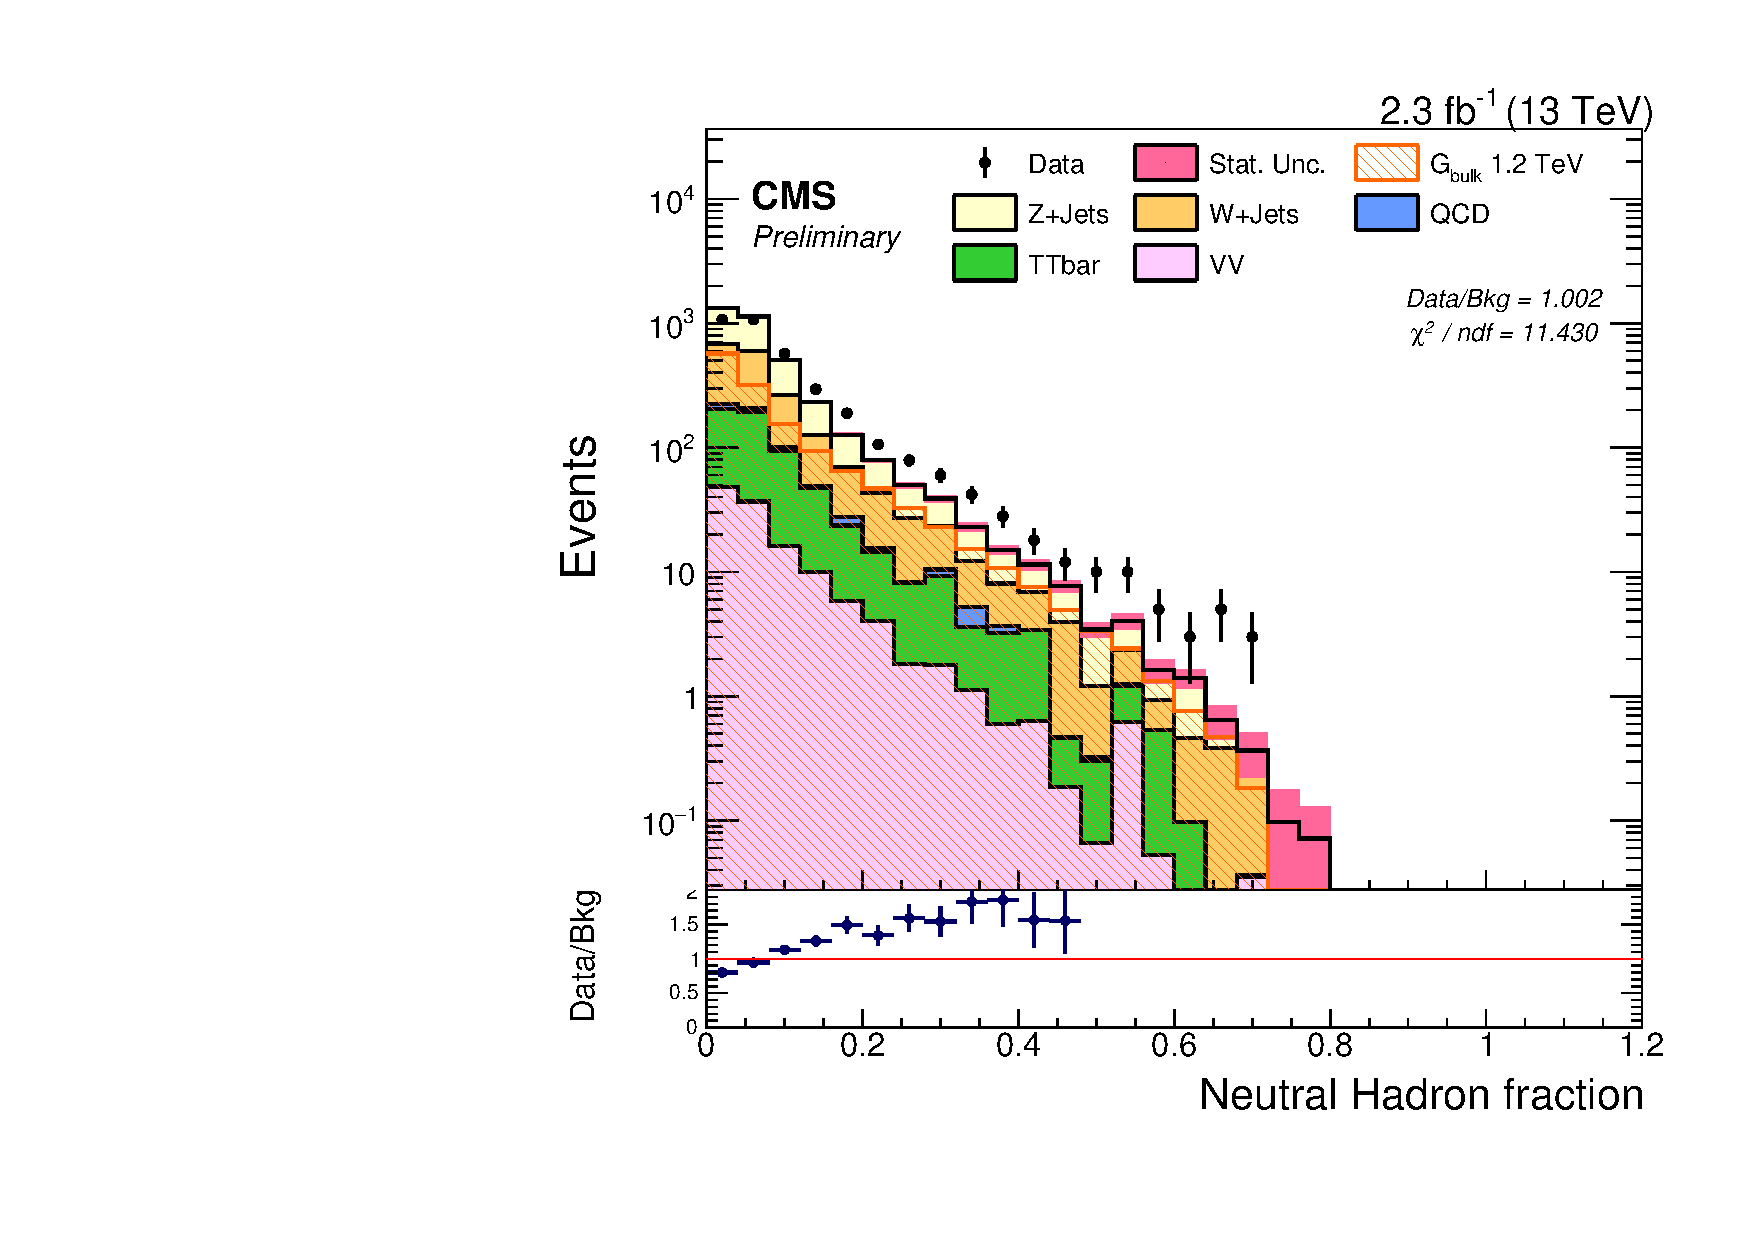
\includegraphics[width=230pt]{figuresCONDI/OBj/LOG_can_h_nhf.pdf} \\
\end{tabular}
\label{fig:jetclen}
\end{figure}

In addition jet energy resolution smearing factors reported in Table \ref{tab:JER},  were applied in the simulation aiming to improve the difference between Data and MC.

\begin{table}[!ht]
\begin{small}
\begin{center}
\caption{Jet energy resolution scaling factors and uncertainty.}
\label{tab:JER}
\begin{tabular}{cc} \hline
$\left| \eta \right|$ region  & Data/MC SF  \\ \hline
0.0-0.5 &  1.095 $\pm$ 0.018  \\
0.5-0.8  &  1.120 $\pm$ 0.028\\
0.8-1.1  &  1.097 $\pm$ 0.017 \\
1.1-1.3  &  1.103 $\pm$ 0.033 \\
1.3-1.7  &  1.118 $\pm$ 0.014 \\
1.7-1.9  &   1.100 $\pm$  0.033\\
1.9-2.1 &  1.162 $\pm$ 0.044   \\
2.1-2.3  &  1.160 $\pm$ 0.048 \\
2.3-2.5  &  1.161 $\pm$ 0.060 \\ 
2.5-2.8  &  1.209 $\pm$ 0.059  \\
2.8-3.0  &  1.564 $\pm$ 0.321  \\
3.0-3.2  &  1.384 $\pm$ 0.033  \\
3.2-5.0  &  1.216 $\pm$ 0.050  \\
\end{tabular}
\end{center}
\end{small}
\end{table}

To identify the hadronic decays of boosted V bosons, jets are clustered using the anti-$\kt$ algorithm with a distance parameter $R=0.8$ namely ``AK8 jets''. The leading AK8 jet is required to be inside the tracker acceptance ($\left| \eta\right| <$ 2.4.) and to have $\pt >$ 200 GeV.
The AK8 jet with the highest $\pt$ is associated to the $V \rightarrow q \bar{q}'$ candidate where the two quarks are merged to the same V-jet.
In addition, another collection of jets clustered with the anti-$\kt$ algorithm with a distance parameter $R=0.4$, called ``AK4 jets'', is used primarily for vetoing the presence of b-jets. The AK4 jets are required to have $\pt$ larger than 30 GeV and $\left| \eta\right| <  2.4$. Figure \ref{fig:ak4Multi} shows the ak4jets multiplicity in events that pass the final analysis selection.

\begin{figure}[!ht]
\caption{ak4Jets multiplicity.}
\begin{center}
  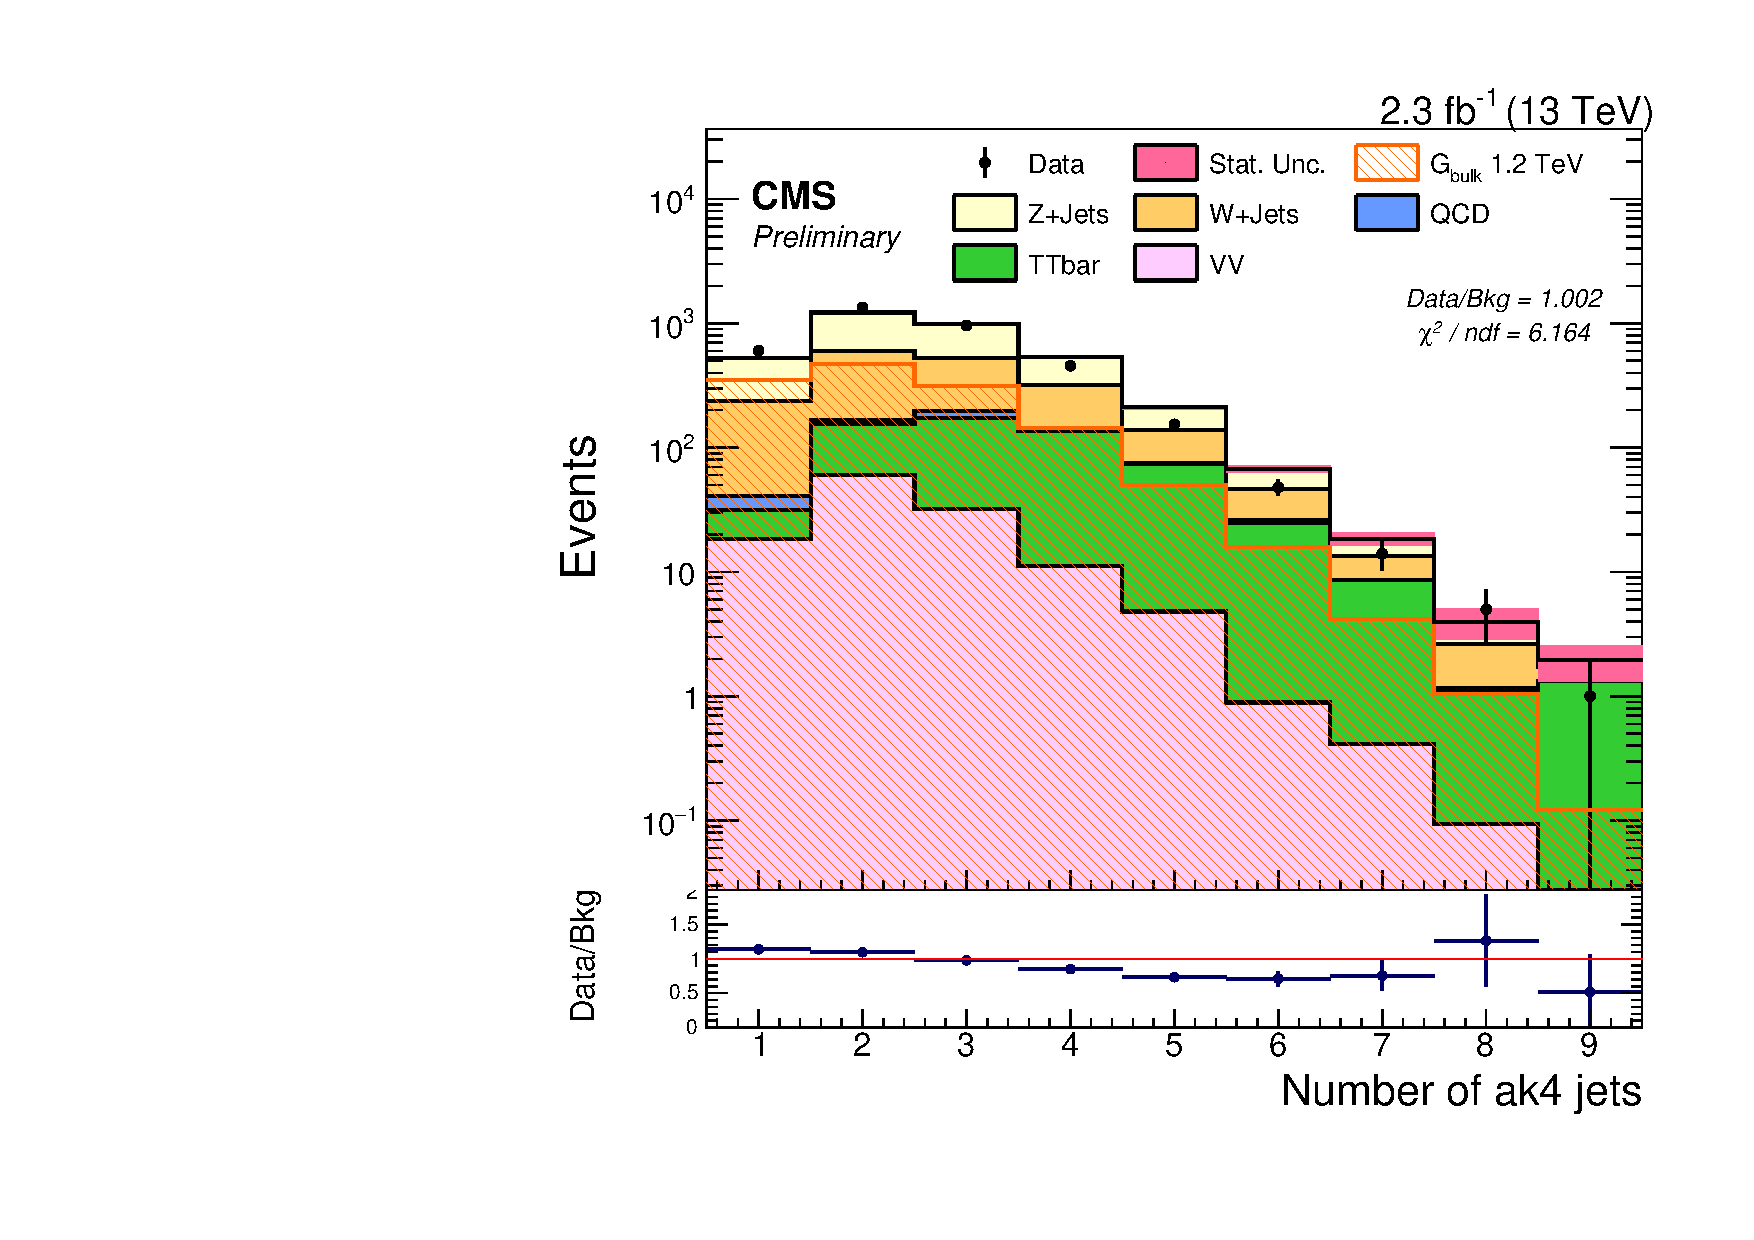
\includegraphics[width=250pt]{figuresCONDI/OBj/LOG_can_h_numjets.pdf}
\end{center}
\label{fig:ak4Multi}
\end{figure}

To identify b-jets, the medium working point of the inclusive combined secondary vertex b-tagging algorithm is applied to the reconstructed AK4 jets. We also required the b-jets to be spatially separated from the AK8 jets by at least $\Delta R = \sqrt{(\Delta \eta)^2+(\Delta \phi)^2}$ = 0.8, where $\Delta \eta$  and $\Delta \phi$ are differences between the b-jet and the AK8 jet directions in the pseudorapidity and the azimuthal angle. b-tagging Efficiency distributions in function of the  $\pt$ and $\left|\eta\right|$ of the jets were derived from simulation. The figure \ref{fig:bjetsscalefactor}  shows the efficiency maps for some MC samples, which are defined as 2D histograms with variable-sized bins in jet $\pt$ and $\left|\eta\right|$.
The ratio of the b-tagging efficiency between data and simulation is used as a scale factor to correct  $t\bar{t}$, V+jets, and signal simulated events.

\begin{figure}[!ht]
\caption{Derived efficiency maps for b-tagging in function of the $\pt$ and $\left|\eta\right|$ of the jet in MC samples (left) $t\bar{t}$ sample  (right) Z +jets sample, for jets with flavor b.}
\begin{tabular}{cc}
  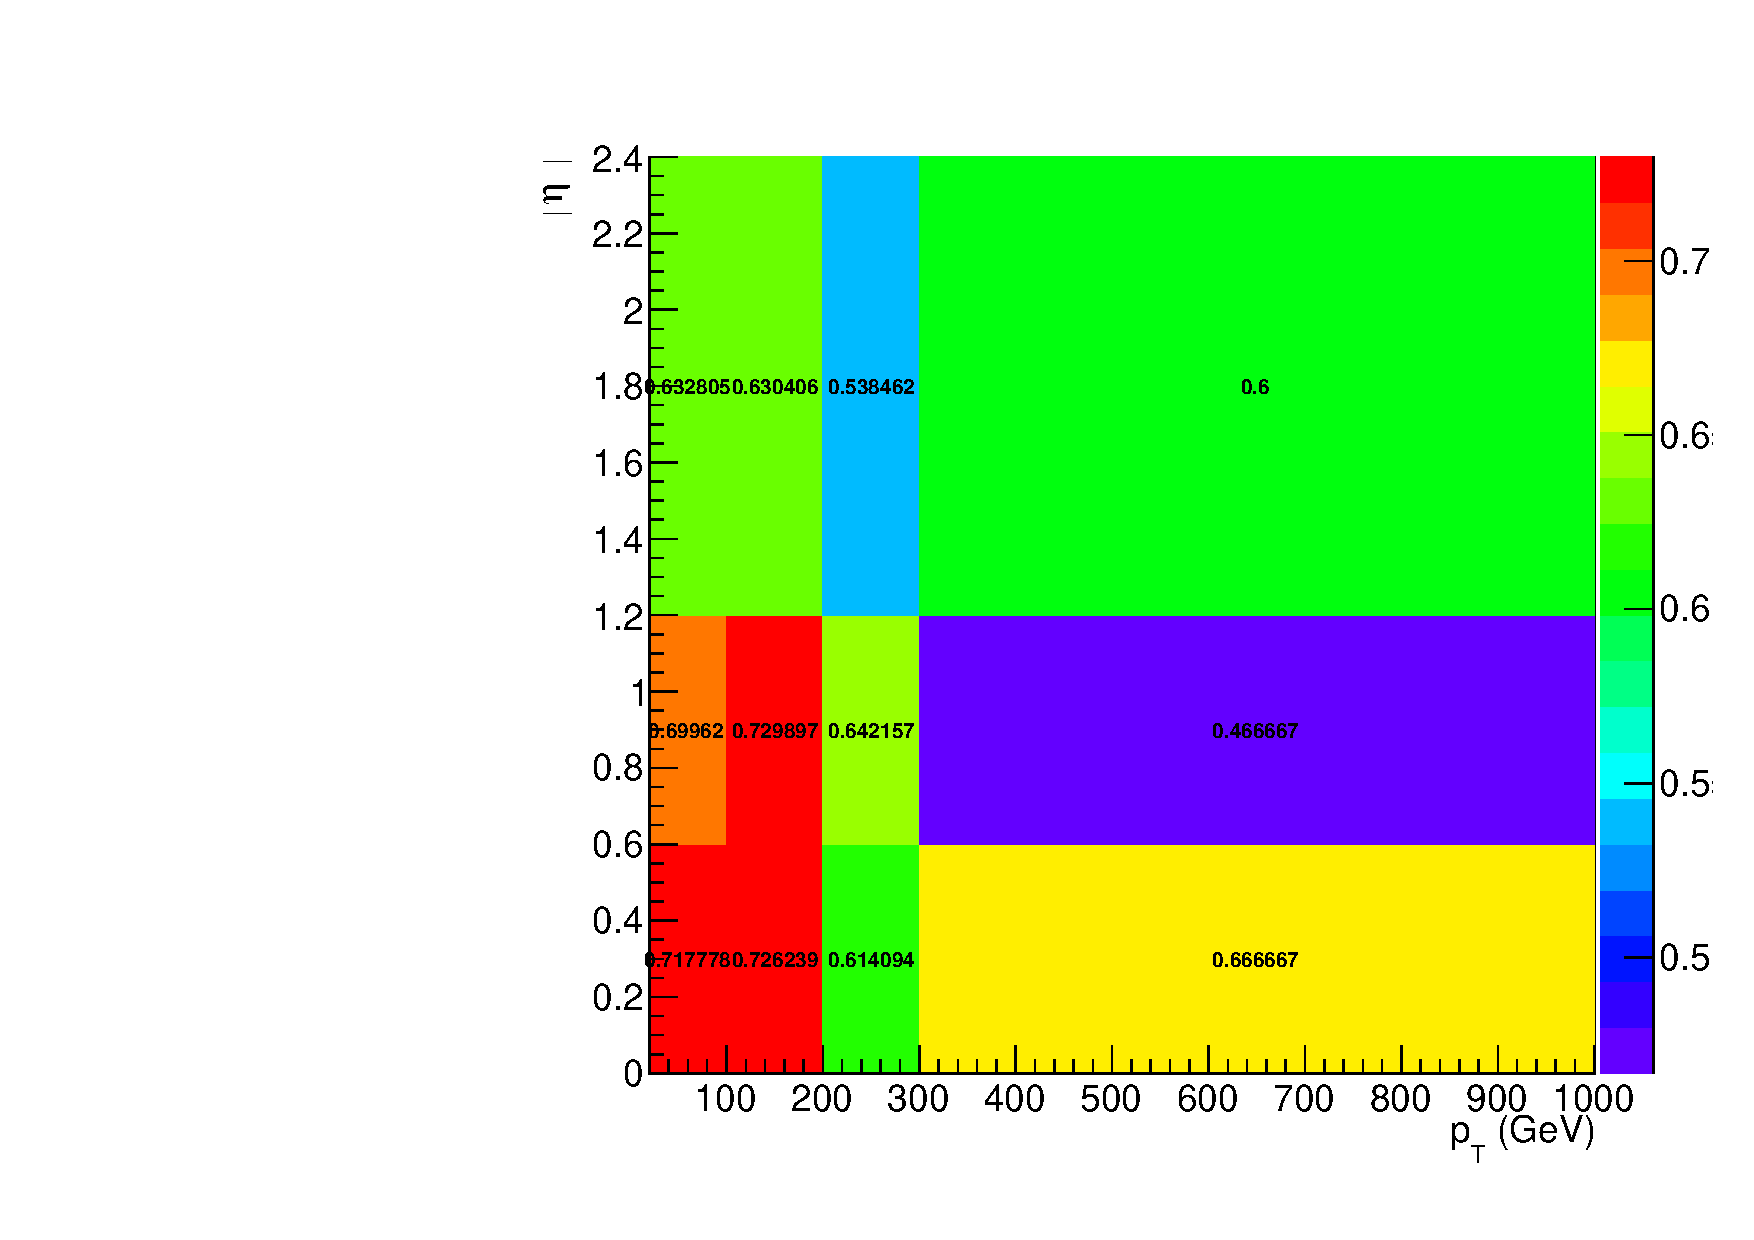
\includegraphics[width=200pt]{figures/SFbtagg/effmapTT.pdf} &
  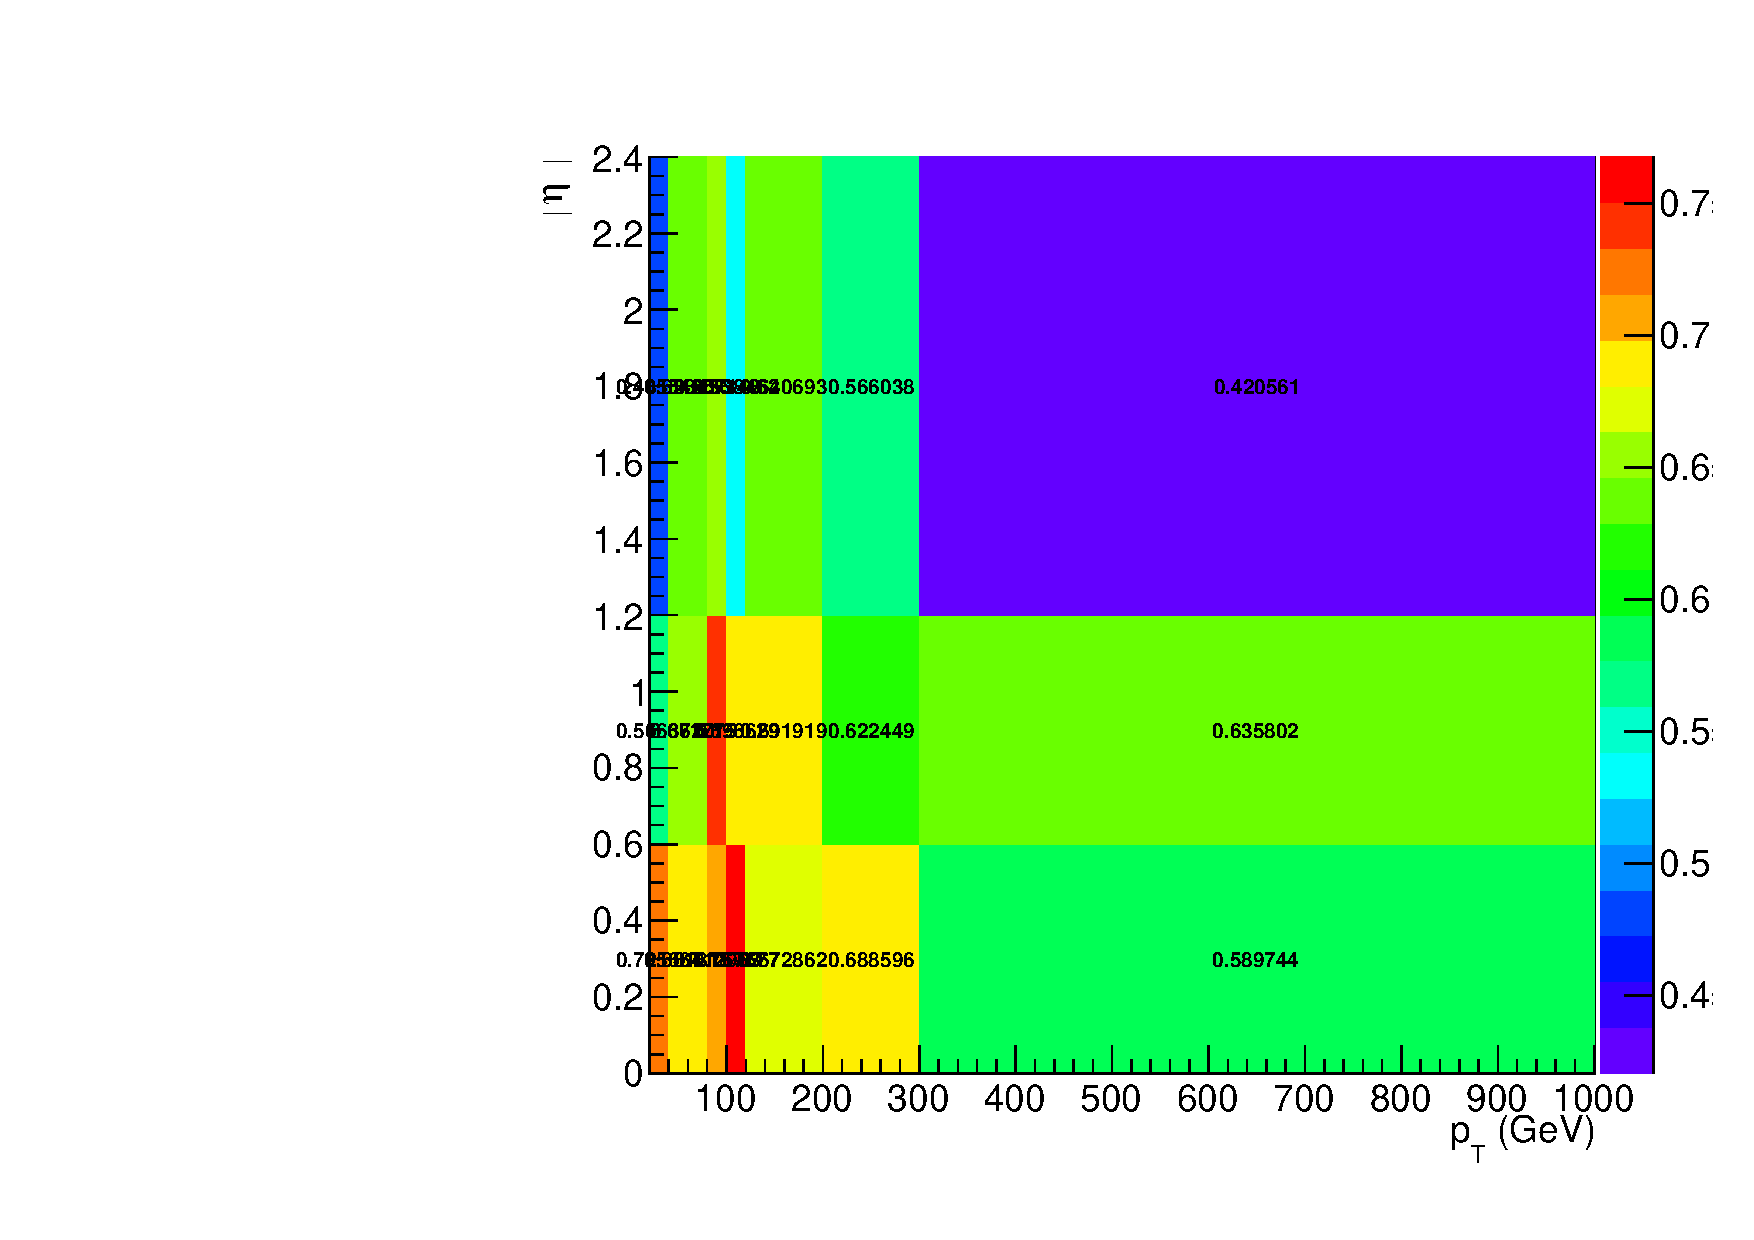
\includegraphics[width=200pt]{figures/SFbtagg/effmapZJ.pdf}\\
\end{tabular}
\label{fig:bjetsscalefactor}
\end{figure}


\section{Hadronic V identification using jet substructure}
\label{sec:HadronicVid}

\par The decay of heavy resonances in dibosons $X \rightarrow VZ$ produce objects with very high $\pt$. When the boost of the V-boson is large enough i.e. $\pt>$200 GeV, the final state hadrons from the decay $V \rightarrow q\bar{q}'$  merge into a single jet. In those cases, the traditional techniques relying on resolved jets are no longer applicable. However, jet substructure methods can be used to identify those jets arising from decays of W, Z or H bosons.
In this analysis, a ``V-tagging" technique based on two jet subtructure methods, pruning  and N-subjettiness, is used in order to discriminate between jets arising from V-decays and those from QCD backgrounds.

\par The leading AK8 jet in the event is considered a V-jet candidate if its pruned mass ($m_{\text{jet}}$), computed from the sum of the four-momenta of the constituents surviving the pruning, falls in the range $65\leq  m_{\text{jet}} \leq105$ GeV. Jets coming from hadronic V decays in signal events are characterized by lower values of $\tau_{21}$  compared to the SM background. To optimize the analysis sensitivity, we distinguish two samples of data:
\begin{itemize}
\item
High Purity (HP) :  $\tau_{21}< 0.45$
\item
Low Purity (LP)  : $0.45 < \tau_{21} < 0.75$
\end{itemize}

Events with $\tau_{21} > 0.75$  are rejected due to very low signal efficiency.
The combined use of the pruned mass and the $\tau_{21}$ allows us to do the V-tagging of a jet with different degrees of purity.
The $\pt$ and $\tau_{21}$ distributions of the highest AK8 jet in the event for data, SM backgrounds, and a bulk graviton
signal sample are shown in Fig. \ref{fig:Vtagg}  after applying a $65\leq  m_{\text{jet}} \leq105$ GeV requirement.
The distribution of $\tau_{21}$  shows some disagreement between data and simulation which is due primarily to a mismodeling of the parton showering \cite{CMS-PAS-EXO-12-021}.

\begin{figure}[!ht]
\caption{ Distribution of $\pt$ (left) and $\tau_{21}$ (right) for the leading AK8 jet in events passing the
final selection in the pruned jet mass signal region for data, SM backgrounds and for a bulk graviton signal sample (1.2 TeV resonance mass and $\tilde{k}$ = 0.5).}
\begin{tabular}{cc}
  \includegraphics[width=230pt]{figures/can_h_ptZjj.pdf} &
  \includegraphics[width=230pt]{figures/can_h_tau21.pdf}\\
\end{tabular}
\label{fig:Vtagg}
\end{figure}

The discrepancies between data and simulation in the jet substructure variables $m_{\text{jet}}$ and $\tau_{21}$ are corrected using scale factors for V-tagging efficiency.
A sample of high-$\pt$ W bosons, which decay hadronically and are reconstructed as a single AK8 jet, was studied in $t\bar{t}$ and single top-quark events. Scale factors for the $\tau_{21}$ selection efficiency are extracted following the method described in Ref. \cite{Khachatryan2014aa}. A simultaneous fit to the jet mass distributions, in both data and simulation, before and after the $m_{\text{jet}}$ and $\tau_{21}$ requirements, is performed to separate the W-signal from the combinatorial components in the top-enriched sample. The fit results are used to extract data-to-simulation efficiency scale factors to identify an isolated hadronic W boson. The scale factors are reported in Table \ref{tab:VtaggSF} and are used to correct the total signal efficiency. The uncertainty on those scale factors is then assigned as systematic uncertainty of the method.

\begin{table}[h!]
 \centering
  \caption{Scale factors for the $\tau_{21}$ efficiency selection derived from data and simulation in a top-quark enriched sample.}
  \label{tab:VtaggSF}
  \begin{tabular}{cc}
\hline
$\tau_{21}$ Selection                 &          Efficiency scale factor          \\
\hline
$\tau_{21} < 0.45$                    &          $0.942 \pm 0.063$                  \\
$0.45 < \tau_{21} < 0.75$             &          $1.268 \pm 0.332$                   \\
\hline
\end{tabular}
\end{table}



\section{Muons}

Muons candidates are reconstructed by associating track measurements in the inner tracker and in the muon system. A set of requirements based on the impact parameter of the track and on the number of hits recorded in the silicon tracker and in the muon chambers have to be fulfilled in order to identify loose muons(referencia). The resulting muons are required to have $\pt > 10$ GeV and $\left| \eta\right| <$ 2.4. To reject nonprompt or misidentified leptons, requirements are imposed on the isolation criteria, based on the sum of deposited energies. The relative isolation parameter (RelIso) is defined as the contributions from the total transverse momentum of all charged hadrons, the transverse energies ($\ET$)  of all photons, and the $\ET$ of all neutral hadrons reconstructed by the PF algorithm within a cone of radius $\Delta R < 0.4$ centered on the muon  track direction, divided by the muon track $\pt$. Identified muons with RelIso values below 0.25 are considered isolated and used in the analysis. Table \ref{tab:MuonID} summarize the criteria used to identify muons.

\begin{table}[h!]
 \centering
  \caption{Muon identification criteria.}
  \label{tab:MuonID}
  \begin{tabular}{|c|p{15cm}| }
\hline
Variable                 &          Criteria          \\
\hline
ID                    &          Loose muon : particle identified as a muon by the Particle-Flow event reconstruction, and that is also reconstructed either as a global-muon or as an arbitrated tracker-muon.    \\ \hline
Isolation             &          PF-based combined relative isolation (RelIso) with $\Delta \beta$ correction, less than 0.25                   \\
\hline
\end{tabular}
\end{table}

In order to reduce electroweak backgrounds (W+jets), we reject events that contain identified muons. Some scale factors (SF) was derived centrally to improve the agreement between data and MC due to identification and Isolation of the muons. We use the SF to reweight the events that contain muons in the following way:
First we define a weight called \emph{muonWeight},  which is equal to 1 for the events that do not contain muons. For the events that contains muons the weight will be:
\begin{eqnarray}
\text{muonWeight} = 1-\text{SF}
\end{eqnarray}
As the SFs are numbers close to 1, the possible outcomes will be:
\begin{itemize}
\item
if SF $<1$ then the muonWeight gives a small positive number
\item
if SF  $=1$ then the muonWeight = 0 (is like apply the veto)
\item
if SF $>1$ then the  muonWeight gives a small negative number
\end{itemize}
We use the equivalence ( muonWeight = 1 $\equiv$ No veto in the event) and (muonWeight = 0 $\equiv$ veto the event)

An association between the reconstructed and the generated muons was performed using a geometrical matching with a cone of $\Delta R(\text{recoMuon},\text{genMuon}) = 0.1$. To resolve ambiguities in the matching, among all the possible combinations, we choose the minimum $\Delta R$ in the calculation. In the figure \ref{fig:Match} we show the minimum $\Delta R$ between the reconstructed and generated muons for a MC signal sample of 1 TeV after apply the final selection of the analysis. The application of the SF is base on kinematic information ($\pt$,$\eta$) of the reconstructed muons that pass the MC matching, taking in account the generator level information of the muons in this process.

\begin{figure}[!ht]
\caption{Minimum $\Delta R$ between reconstructed and generated muons for a signal mass point of 1 TeV.}
\begin{center}
  \includegraphics[width=250pt]{figuresCONDI/OBj/matchingmuons.pdf} 
\end{center}
\label{fig:Match}
\end{figure}

\section{Electrons}

Electrons candidates are reconstructed by associating a charged particle track with an ECAL supercluster, including energy depositions from final-state radiation. The resulting electron candidates are required to have $\pt > 10$ GeV, $\left| \eta\right| <$ 2.4, and to satisfy identification criteria designed to remove photon conversions, jets misidentified as electrons, and electrons from semileptonic decays of bottom and charm quarks. Identified electrons with RelIso values below 0.1 are considered isolated and used in the analysis. Events with identified electrons are vetoed to reduce W+jets background. SFs were derived centrally to improve the agreement between data and MC due to identification and Isolation of the electrons. A MC matching was implemented in the reconstructed electrons aiming to applying the SF taking in account the generator level information of the electrons. The method to apply the SFs over the MC samples to reweight the event was explained in the muons section.


\section{Taus}

The hadronic tau ($\tau_{h}$) decays are reconstructed and identified using the hadrons-plus-strips (HPS) algorithm. The algorithm is designed to reconstruct individual decay modes of the tau lepton, taking advantage of the PF algorithm. It also discriminate $\tau_{h}$ decays from quark and gluon jets, and from electrons and muons. In addition, tau-isolation requirements complement the identification process. Identified taus are required to have $\pt > 20$ GeV and $\left| \eta\right| <$ 2.3 to be used in the analysis.
Events with identified taus are removed in order to disminished W+jets background. We consider for the tau ID efficiency, the ratio between data and MC equal to 1, with an uncertainty of 6$\%$. This recommendation is valid for all isolation discriminators, $\pt$ and $\eta$ range, in Run-2 analyses. 


\section{Photons}\label{photons}

Photons candidates are reconstructed by clustering spatially correlated energy deposits in the ECAL. Photon identification is based on two main categories of observables: shower-shape and isolation variables which help to discriminate among signal photons and photons that arise from neutral mesons produced in jets or electrons misidentified as photons. Identified photons are required to have $\pt > 15$ GeV and $\left| \eta\right| <$ 2.5 to be used in the analysis. In order to reduce Z +$\gamma$ +jets and W + $\gamma$ +jets backgrounds  we reject events that contain photons.
Photons candidates are required to have a minimum $\pt$ of 15 GeV and $\left| \eta\right| < $2.5.
With the objective to identify photons we use a loose cut-based working point identification.
SFs were derived centrally to improve the agreement between data and MC due to identification and Isolation of the photons. We apply properly those scale factor over the MC samples to reweight the event as was explained in the muons section.

\section{Transverse mass}\label{MT}
The hadronic V-boson candidate ($V \rightarrow q \bar{q}'$) is reconstructed from the AK8 jet with the highest $\pt$. Due to the invisible decay of the Z boson ($Z \rightarrow \nu \bar{\nu}$), the reconstruction of the resonance mass is not directly viable and its total momentum can be constrained only in the plane transverse to the beam direction. Therefore, we will use as the final discriminant a quantity called ``transverse mass'', defined by
\begin{eqnarray*}
M_{VZ}^{T} = \sqrt{2 p_{T} \MET \left( 1-\cos(\Delta \phi)\right)}
\end{eqnarray*}
where $p_{T}$ is the transverse momentum of the AK8 Jet and $\Delta \phi$ is the angle between the jet $\pt$ and the $\MET$ vector.


\chapter{Event Selection}\label{selection}

The data used in this analysis was collected online using a trigger designed to record events that
contain large values of $\HT^{\text{miss}}$ and $\MET$. The details of the trigger were explained in the chapter \ref{samples}. Offline, all events are required to have at least one primary vertex reconstructed within a 24 cm window along the beam axis, with a transverse distance from the nominal pp interaction region of less than 2 cm. In the presence of more than one vertex passing these requirements, the primary-event vertex is chosen to be the one with the highest total $\pt^{2}$, summed over all the associated tracks.

In the signal region we select events that contain highly energetic AK8 jets and large missing transverse energy.
An event falls into this category if the AK8 jets have $\pt >$ 200 GeV, $\left| \eta\right| <$ 2.4, $65\leq  m_{\text{jet}} \leq105$ GeV and $\tau_{21}<0.75$. For the missing energy, we require $\MET> 250$ GeV. If the selected event contains more than one AK8 jet with the previous requirements, the jet with the largest $\pt$ is chosen in order to calculate the transverse mass variable.
Also, a lower threshold of 600 GeV in the transverse mass is required in the selected events. Below this value, a new resonance would not be massive enough to produce a large fraction of boosted V bosons, resulting in a low value of the selection efficiency.

Background from leptonic W boson decays is reduced through rejection of events with isolated leptons (electrons, muons, taus) identified with loose selection criteria. Events containing b-jets are vetoed in the analysis in order to suppress $t\bar{t}$ background. Events containing identified photons are reject to reduce V +$\gamma$+jets backgrounds. To supress QCD multijet background in which large $\MET$ could arise,
the minimum azimuthal angle between the $\MET$ direction and the AK4 jets with $\pt$ greater than 30 GeV is required to be greater than 0.5. 
Table \ref{tab:finalsel} summarize the final selection chosen in the analysis.

In order to set object disambiguation between possible VZ candidates, we use as a selection criteria the candidate with the highest transverse momentum in the event.

The signal efficiency in each category ($\varepsilon_{\text{cat}}$) is defined as the ratio between the number of signal events after the hole analysis selection in a chosen category ($N^{\text{cat}}_{\text{sel}}$) over the total number of generated signal events ($N_{\text{gen}}$).

\begin{eqnarray}
\varepsilon_{\text{cat}} = \dfrac{N^{\text{cat}}_{\text{sel}} }{N_{\text{gen}}},\qquad  \text{cat = HP,LP} 
\end{eqnarray}

The signal efficiencies are evaluated for the full analysis selection inside the VZ-enriched ($65 \leq  m_{\text{jet}} \leq 105$ GeV) mass windows, and are shown in figure \ref{fig:eff} for the bulk graviton signal model for several mass points and different categories. The high purity efficiency drops at high values of the resonance mass due to the inefficiency of the N-subjettines and jet mass selection; this is partially recovered in the low purity category.

Figure \ref{fig:controlplots1} shows a set of comparison plots between data and simulation for interesting variables in the analysis. The final analisys selection except for a loose requirement in the mass of the jet $40 \leq  m_{\text{jet}} \leq 220$ GeV was used to produce the plots in order to observe regions that will be employed for background estimation (sideband regions). In general a good agreement between data and simulation is observed in the control plots.

\def\arraystretch{1.2}
\begin{table}[h]
\begin{footnotesize}
\caption{Final analysis selection.}
\label{tab:finalsel}
\begin{tabular}{|c|cc|}
\hline
\textbf{Selection}                     &                                       &       \textbf{Value}                                                   \\  \hline
High Level Trigger                     &                                       &      $\verb|PFMETNoMu90_JetIDCleaned_PFMHTNoMu90_IDTight|$      \\ 
                                       &                                       &       OR $\verb|HLT_PFMET170_*|$                               \\ \hline
                                       &                                       &      Type-I PF MET                                            \\      
\raisebox{1.5ex}[0pt]{$E_{\text{T}}^{\text{miss}}$} &                          &      $p_{T} > 250$ GeV                                        \\ \cline{1-3}
                                       &                                       &      PFJetID Loose                                            \\  
                                       &                                       &      $p_{T} > 200$ GeV, $\left|\eta\right|< 2.4$               \\  
                                       & \raisebox{1.5ex}[0pt]{AK8Jets}              &      $ 65 < m^{\text{pruned}}_{\text{jet}} < 105$ GeV           \\  
\raisebox{1.5ex}[0pt]{Jets}            &                                       &      CHF $> 0.1$, NHF $< 0.8$                                   \\  \cline{2-3}
                                       &                                       &      PFJetID Loose                                            \\  
                                       &                                       &      $p_{T} > 30$ GeV, $\left|\eta\right|< 2.4$               \\  
                                       &  \raisebox{1.5ex}[0pt]{AK4Jets}       &      CHF $> 0.1$, NHF $< 0.8$        \\
                                       
                                       &                                       &      $\text{min}\Delta \phi(\text{AK4Jet},\MET) >$ 0.5             \\
                                       &                                       &      b-tag Veto : CSV $>$ 0.8 
 
                           \\  \cline{1-3}
Leptons (electrons, muons, taus)                                &                                       &      Veto                                                        \\  \cline{1-3}
Photons                                &                                       &      Veto                                                      \\ \cline{1-3}
VZ candidate transverse mass           &                                       &      $M^{\text{T}}_{\text{VZ}} > 600$ GeV                      \\ \cline{1-3}
\end{tabular}
\end{footnotesize} 
\end{table}

\begin{figure}[!ht]
\caption{ Signal efficiency for $G_{Bulk} \rightarrow ZZ \rightarrow $ jet + $\MET$ for different mass points and different categories after the final analysis selection.}
\begin{center}
  \includegraphics[width=280pt]{figuresARC/sigeff/efficiency.pdf}
\end{center}
\label{fig:eff}
\end{figure}



\begin{figure}[!ht]
\caption{Top:(left) AK8 Jet transverse momentum. (right) Missing transverse energy. Center: (left) AK8 Jet pseudorapidity. (right) min $\Delta \phi$ distribution. Bottom: (left) Pruned jet mass. (right) Candidate transverse mass. The plots show the comparison between data(black dots) and simulation. The simulation is composed by different backgrounds: Z+jets(light yellow), W+jets(orange), $t\bar{t}$(green), QCD multijets(light blue) and diboson(light pink). The statistical uncertainty is shown in dark pink. In addition a Bulk graviton signal sample of 1.2 TeV is shown by the orange hatch region. The figure also show the ratio of the histograms (data/simulation) and the $\chi^{2}/\text{ndf}$ value as a figure of merit.}
\begin{tabular}{cc}
  \includegraphics[width=180pt]{Chapter6_plots/LOG_can_h_ptZjj.pdf} &
\includegraphics[width=180pt]{Chapter6_plots/LOG_can_h_metpt.pdf}\\
\includegraphics[width=180pt]{Chapter6_plots/LOG_can_h_yZjj.pdf} &
\includegraphics[width=180pt]{Chapter6_plots/LOG_can_h_minabsdeltaphi.pdf}\\
\includegraphics[width=180pt]{Chapter6_plots/can_h_massZjj.pdf} &
\includegraphics[width=180pt]{Chapter6_plots/LOG_can_h_candTMass.pdf}\\
\end{tabular}
\label{fig:controlplots1}
\end{figure}

\chapter{Background Modeling}\label{bkg_estimate}

To perform an accurate prediction of the SM backgrounds we used a data-driven strategy called \emph{alpha ratio method} that will be discuss in the section \ref{alpha}. The dominant background contribution in the analysis  originates from the V+jets processes (they represent the 83$\%$ of the total background). The subdominant contributions come from $t\bar{t}$, diboson (WW/WZ/ZZ), and QCD multijets. The subdominant contribution yields and the transverse mass shapes ($M_{VZ}^{T}$) are primarily taken from simulation. Table \ref{tab:backgrounds} summarize the background categories.

\begin{table}[!ht]
\begin{center}
\caption{Background categories.}
\label{tab:backgrounds}
\begin{tabular}{lc} \hline
Category & Backgrounds \\ \hline
Dominants &  $W$+jets($W \rightarrow \ell \nu$), $Z$+jets ($Z\rightarrow \nu \nu$)  \\
Subdominants   &  Multijets, $t\bar{t}$, dibosons ($WW$/$WZ$/$ZZ$) \\ \hline
\end{tabular}
\end{center}
\end{table}

To determine the dominant V+jets background in the signal region ($m_{\text{jet}} \in \left[65,105 \right]$ GeV), a signal-free sideband region is defined in the mass of the hadronic V candidate by the interval  $m_{\text{jet}} \in \left[40,65 \right] \cup \left[135,220\right]$ GeV. The region $m_{\text{jet}} \in \left[105,135 \right]$ GeV is not used in order to avoid any bias in the $M_{VZ}^{T}$ shape due to possible contributions from new resonances in the HZ final state, in which the Higgs bosons would decay to a pair of b-quarks. Table \ref{tab:jetmassregions} summarize the different jet mass regions used for the background modeling.

\begin{table}[!ht]
\begin{center}
\caption{Jet mass regions.}
\label{tab:jetmassregions}
\begin{tabular}{lc} \hline
Region & Interval (GeV) \\ \hline
Lower sideband  (LSB) &  $\left[40,65 \right]$  \\
Lower signal  (SR)  &  $\left[65,105 \right]$ \\ 
Upper signal (Higgs) & $\left[105,135 \right]$   \\
Upper sideband (USB) & $\left[135,220 \right]$  \\ \hline
\end{tabular}
\end{center}
\end{table}

In general, we experience low statistics in data, particularly in the tail of transverse mass distribution, which is the main observable in order to determine any possible signal of new physics. For those cases unbinned maximum likelihood (ML) fits are preferred due to robustness (statistically more powerful) and to avoid the information loss and arbitrariness of the binning procedure \cite{Verkerke:2003ir}. Therefore, in the analysis, we perform all the fits using the unbinned ML method.

\section{Alpha ratio method}\label{alpha}

The alpha ratio method is based on the extrapolation of the background shape and yield from the jet pruned mass sideband to the signal region. The method relies on the assumption that the correlation between $M_{VZ}^{T}$ and the  jet pruned mass for the dominant background in data is reasonably well reproduced in simulation. The advantage of this approach is that most systematic uncertainties cancel in the ratio.
The total background prediction (normalisation and shape) as a function of the reconstructed resonance mass, $M_{VZ}^{T}$, is obtained separately for each purity category according to the formula:

\begin{eqnarray}
N_{\text{total}}^{\text{signal}}(M_{VZ}^{T}) &=& N_{\text{DB}}^{\text{signal}}(M_{VZ}^{T}) + N_{\text{SB}}^{\text{signal}}(M_{VZ}^{T})\\
                                        &=& \underbrace{N_{\text{data}}^{\text{sideband}}(M_{VZ}^{T}) \times (1-R_{0}(M_{VZ}^{T}))\times \alpha^{MC}(M_{VZ}^{T})}_{\text{Shape}}\times \underbrace{F_{DB}}_{\text{Norm}} \nonumber  \\                                        &+& N_{\text{SB}}^{\text{signal}}(M_{VZ}^{T})  \nonumber
\end{eqnarray}

where

\begin{itemize}
\item
$N_{\text{total}}^{\text{signal}}(M_{VZ}^{T})$ is the total background prediction in the signal region;
\item
$N_{\text{DB}}^{\text{signal}}(M_{VZ}^{T})$ is the dominant background prediction in the signal region (W/Z + jets);
\item
$N_{\text{SB}}^{\text{signal}}(M_{VZ}^{T})$ is the background prediction in signal region for the sum of the subdominant backgrounds ($t\bar{t}$, multijets, dibosons);
\item
$N_{\text{data}}^{\text{sideband}}(M_{VZ}^{T})$ is the $M_{VZ}^{T}$ distribution in data for the sideband region;
\item
$R_{0}(M_{VZ}^{T})= N_{\text{SB}}^{\text{sideband}}(M_{VZ}^{T})/N_{\text{data}}^{\text{sideband}}(M_{VZ}^{T})$ is the fraction of subdominant backgrounds in the sideband region with respect to the total background in the sideband region (i.e. data). The $1-R_{0}(M_{VZ}^{T})$ multiplicative term represents the substraction of the subdominant contribution from the data in the sideband region;
\item
$\alpha^{MC}(M_{VZ}^{T})= N_{\text{DB}}^{\text{signal}}(M_{VZ}^{T})/N_{\text{DB}}^{\text{sideband}}(M_{VZ}^{T}) $ is the dominant background prediction in the signal region divided by the one in the sideband region, calculated from MC. It represents the transfer function (from sideband to signal region) used to correct the data in the sideband region and extract the dominant background’s $M_{VZ}^{T}$ shape.
\item
$F_{DB}$ is an overall scale factor used to set the normalisation of the dominant background prediction.
\end{itemize}

In summary, the method is divide in two parts, the shape and the normalization prediction for the dominant backgrounds. We will detail each in the following sections. The alpha ratio method is the standard strategy for background estimation used by CMS in similar searches \cite{CMS:2013xea,CMS-PAS-EXO-12-022, CMS-PAS-EXO-15-002}. 


\subsection{Background normalization}

The $m_{\text{jet}}$ distribution is modeled with analytic functions on simulation, considering separately the dominant and subdominant backgrounds. The overall dominant background normalization in the signal region is determined from a fit to the $m_{\text{jet}}$  distribution in the sideband region, after fixing both the shape and the normalization of the subdominant backgrounds. Table \ref{tab:functions} show the functional forms employed to describe the jet pruned mass distribution.

\def\arraystretch{2.0}
\begin{table}[!ht]
\begin{center}
\caption{Analytic functions to fit the jet pruned mass distribution.}
\label{tab:functions}
\begin{tabular}{lcc} \hline
Name & Description & Function \\ \hline
\textbf{ErfExp} & An exponential times an error function & $e^{a} \cdot \frac{1 + \text{Erf}\left((x-b)/w \right)}{2}$ \\
\textbf{Gaus2}  &  The addition of two gaussians & $f_{0}e^{-(x-a)^{2}/2s^{2}} + (1-f_{0})e^{-(x-b)^{2}/2s^{2}}$ \\ \hline
\end{tabular}
\end{center}
\end{table}

To verify that the W + jets and Z +jets samples have the same shape and that we can treat them together as a dominant background, we perform a cross-check, fitting them separately as is shown in Figure \ref{fig:Vjets}. For the normalization procedure we follow the next steps:

\begin{itemize}
\item
We fit the dominant backgrounds with the \textbf{ErfExp} model in the total jet pruned mass distribution, as it can be observed in the top-left side of the figures \ref{fig:fitprunedHP}, \ref{fig:fitprunedLP}.
\item
We fit the subdominant backgrounds with the \textbf{Gaus2} model in the total jet pruned mass distribution, as it can be observed in the top-right side of the figures \ref{fig:fitprunedHP}, \ref{fig:fitprunedLP}.
\item
We use an extended model adding the PDFs of the dominant and subdominants backgrounds. For the dominant backgrounds we let both the parameters of the normalization and shape float and for the subdominant backgrounds we fix the parameters of the normalization and shape. Then we fit the extended model to the data in sidebands.
\item
Using the results of the fits, we predict the shape and the normalization ($F_{DB}$) of the dominant backgrounds in signal region. Figures \ref{fig:fitprunedHP}, \ref{fig:fitprunedLP}, bottom side, show the prediction  in comparison with data. In addition, we can extract the estimation of the total yields in signal region as is reported in table \ref{tab:backyields4}.
\end{itemize}

The characterization of the jet pruned mass with the analytic functions was evaluated in simulation and compared against alternative functions. To consider the mis-modelling of the pruned jet mass, an uncertainty was included as a systematic error that ranges between 15-20 $\%$. The expected and observed number of events in the signal region is given in Table \ref{tab:backyields4}; the result is reported for the HP and LP categories.

\begin{table}[!ht]
\begin{center}
\caption{Expected and observed background yields in signal region.}
\label{tab:backyields4}
\begin{tabular}{lcccc} \hline
Category & Background &  Expected & Observed & Syst. Uncer.\\ \hline
HP & Dominant + Sub-dominant  &  544 $\pm$ 40  & 507 & 20.5 $\%$  \\
LP & Dominant + Sub-dominant  &  820 $\pm$ 53 & 806  &  15.5$\%$  \\ \hline
\end{tabular}
\end{center}
\end{table}

\subsection{Background shape}

Evidence of a new resonance decaying into disboson ($VZ$) would appear as a localized excess in the transverse mass distribution. Because of this, it is essential to perfom a good estimtaion of the background shape in the $M_{VZ}^{T}$ variable. Due to the correlation between the jet pruned mass and the transverse mass variables, the selections on the $m_{\text{jet}}$ reported in table \ref{tab:jetmassregions} define the sideband and the signal regions in the $M_{VZ}^{T}$ distributions. The analytic model selected to estimate the background shape of the transverse mass distribution is the \textbf{ExpTail}:
\begin{eqnarray}
F_{\text{ExpTail}}(x) = e^{-x/(a+bx)}
\end{eqnarray}
The choice of the functional forms for the VZ transverse mass for different categories is shown in table \ref{tab:trasnversefunctions}.
\begin{table}[h]
\begin{center}
\caption{Summary of the shapes used for fit the $M_{VZ}^{T}$ spectra of each category.}
\label{tab:trasnversefunctions}
\begin{tabular}{lcccc} \hline
Category & Fit Function & Regions & Sample \\ \hline
HP  &  ExpTail  &  signal and sideband  & Data and MC \\
LP  &  ExpTail  &  signal and sideband  & Data and MC \\ \hline
\end{tabular}
\end{center}
\end{table}

In order to predict the shape of the dominant backgrounds we follow the next steps:

\begin{itemize}
\item
We fit the subdominants backgrounds with an \textbf{ExpTail} model in sideband and signal region. After the fit we fix all the parameters of the model.
\item
We substract the subdominant backgrounds from data in the sideband region.
\item
We perform a simultaneous fit using the \textbf{ExpTail} model for the dominant background in the signal and sideband region and for the data in sideband region.
After the fit we fix all the parameters of the model. Figures \ref{fig:fits3}, \ref{fig:fits4} show the results of the fits. The top side shows the dominant backgrounds fits in sideband and signal region and the right-center side show the data fit in sideband region.
\item
We extract the alpha transfer function using the fits of the dominant backgrounds in sideband and signal region. $\alpha^{MC}(M_{VZ}^{T})= N_{\text{DB}}^{\text{signal}}(M_{VZ}^{T})/N_{\text{DB}}^{\text{sideband}}(M_{VZ}^{T})$.  Figures \ref{fig:fits3}, \ref{fig:fits4} show the alpha transfer function for high and low purity categories respectively.
\item
We predict the shape of the dominant backgrounds in signal region just correcting the $M_{VZ}^{T}$ distribution of the data in sideband region with the transfer function. Figures \ref{fig:fits3}, \ref{fig:fits4} show the final prediction in comparison with data. In those plots the normalization factor was already applied.
\end{itemize}

\begin{figure}[!ht]
\caption{ Top : Z/W +jets fits in the HP category. Center : Z/W +jets fits in the LP category. Bottom : Comparison between the Z +jets and W +jets fits.}
\begin{tabular}{cc}
  \includegraphics[width=220pt]{figuresARC/Vjets/ZjetsHP.pdf} &
\includegraphics[width=220pt]{figuresARC/Vjets/WjetsHP.pdf}\\
  \includegraphics[width=220pt]{figuresARC/Vjets/ZjetsLP.pdf} &
\includegraphics[width=220pt]{figuresARC/Vjets/WjetsLP.pdf}\\
  \includegraphics[width=220pt]{figuresARC/Vjets/VjetsHP.pdf} &
\includegraphics[width=220pt]{figuresARC/Vjets/VjetsLP.pdf}\\
\end{tabular}
\label{fig:Vjets}
\end{figure}

\begin{figure}[!ht]
\caption{ Fit of the jet pruned mass in the HP category. Top: (left) Dominant MC background fit with the ErfExp function (right) Subdominant MC background fit with the Gaus2 function. Bottom: Distribution of the jet pruned mass in the HP categories. All selections are applied except the final $m_{\text{jet}}$ signal window requirement. Data are shown as black markers. The contribution of the V+jets background is extrapolated from the sideband to the signal region.}
\begin{tabular}{cc}
  \includegraphics[width=250pt]{figuresARC/Vjets/DomHP.pdf} &
\includegraphics[width=250pt]{figuresARC/Vjets/SubDomHP.pdf}\\
\end{tabular}
\begin{center}
  \includegraphics[width=270pt]{figuresARC/Vjets/dataMjUB3HP.pdf}
\end{center}
\label{fig:fitprunedHP}
\end{figure}

\begin{figure}[!ht]
\caption{ Fit of the jet pruned mass in the LP category. Top: (left) Dominant MC background fit with the ErfExp function (right) Subdominant MC background fit with the Gaus2 function. Bottom: Distribution of the jet pruned mass in the LP categories. All selections are applied except the final $m_{\text{jet}}$ signal window requirement. Data are shown as black markers. The contribution of the V+jets background is extrapolated from the sideband to the signal region.}
\begin{tabular}{cc}
  \includegraphics[width=250pt]{figuresARC/Vjets/DomLP.pdf} &
\includegraphics[width=250pt]{figuresARC/Vjets/SubDomLP.pdf}\\
\end{tabular}
\begin{center}
  \includegraphics[width=270pt]{figuresARC/Vjets/dataMjUBLP.pdf}
\end{center}
\label{fig:fitprunedLP}
\end{figure}

\begin{figure}[!ht]
\caption{ Fit of the VZ candidate transverse mass in the HP category. Top: (left) Dominant MC background fit in the sideband region (right) Dominant MC background fit in the signal region. Center: (left) alpha transfer function (right) Data fit in the sideband region. Bottom: Final prediction on the background estimation in signal region.
The solid curve represents the background estimation provided by the data-driven
method. The hatched band includes both statistical and systematics uncertainties. The data
are shown as black markers. The bottom panels show the corresponding pull distributions,
quantifying the agreement between the background-only hypothesis and the data. The pull
distribution is defined as the difference between the data and the background prediction, divided by the error on data. The error bars on the points represent the error on data.
}
\begin{tabular}{cc}
\includegraphics[width=150pt]{figuresARC/fits/sbDom_MVZHP.pdf} &
\includegraphics[width=150pt]{figuresARC/fits/sigDom_MVZHP.pdf}\\
\includegraphics[width=150pt]{figuresARC/fits/alphaHP.pdf}&
\includegraphics[width=150pt]{figuresARC/fits/sbData_MVZHP.pdf}\\
\end{tabular}
\begin{center}
  \includegraphics[width=200pt]{figuresARC/fits/finalresultUBHP.pdf}
\end{center}
\label{fig:fits3}
\end{figure}


\begin{figure}[!ht]
\caption{ Fit of the VZ candidate transverse mass in the LP category. Top: (left) Dominant MC background fit in the sideband region (right) Dominant MC background fit in the signal region. Center: (left) alpha transfer function (right) Data fit in the sideband region. Bottom: Final prediction on the background estimation in signal region.
The solid curve represents the background estimation provided by the data-driven
method. The hatched band includes both statistical and systematics uncertainties. The data
are shown as black markers. The bottom panels show the corresponding pull distributions,
quantifying the agreement between the background-only hypothesis and the data. The pull
distribution is defined as the difference between the data and the background prediction, divided by the error on data. The error bars on the points represent the error on data.}
\begin{tabular}{cc}
  \includegraphics[width=150pt]{figuresARC/fits/sbDom_MVZLP.pdf} &
  \includegraphics[width=150pt]{figuresARC/fits/sigDom_MVZLP.pdf}\\
\includegraphics[width=150pt]{figuresARC/fits/alphaLP.pdf}&
\includegraphics[width=150pt]{figuresARC/fits/sbData_MVZLP.pdf}\\
\end{tabular}
\begin{center}
  \includegraphics[width=200pt]{figuresARC/fits/finalresultUBLP.pdf}
\end{center}
\label{fig:fits4}
\end{figure}



\chapter{Signal Modeling}\label{sig_model}

The shape of the reconstructed signal mass is extracted from the bulk graviton and $W'$ samples to model the peak of the resonance. The natural width of the resonance is considered to be  sufficiently small to be neglected when compared to the detector resolution. In the final analysis of the $M_{VZ}^{T}$ spectrum, the discovery potential and the exclusion power depend both on an accurate description of the signal shape. We adopt an analytical description of the signal shape, choosing a single Crystal-Ball function (i.e. a Gaussian
core with power-law low-end tail) to describe the CMS detector resolution. The typical
width of the Gaussian core is about 5$\%$-7$\%$ of the nominal mass. The analytical description
of the signal shape allows us to probe mass points for which there is no generated sample by
interpolating the shape parameter. No appreciable differences have been observed
in the $M_{VZ}^{T}$ signal shape between the low-purity and the high-purity categories.
Table \ref{tab:Bulksignal} and table \ref{tab:Wprimesignals} show the mass points and the fit range for each signal hypothesis. The transverse mass fits in the signal sample are shown in the figures \ref{fig:fits6a},\ref{fig:fits6b}, and \ref{fig:fits7}. Figure \ref{fig:fits9} shows the simulated $M_{VZ}^{T}$ distribution for resonance masses from 800 to 2000 GeV after the interpolation process. The different distributions are normalized to the corresponding efficiencies.

\begin{table}[h]
\begin{center}
\caption{Different mass points to fit the signal shape for Bulk graviton model.}
\label{tab:Bulksignal}
\begin{tabular}{ccc} \hline
Mass point (GeV) & Mean (GeV) &  Fit window (GeV) \\ \hline
800 & 763 & [620,900] \\
1000 & 930 & [670,1190] \\
1200 & 1100 & [720,1424] \\
1400 & 1283 & [850,1657] \\
1600 & 1461 & [1035, 1887] \\
1800 & 1640 & [1168, 2112] \\
2000 & 1819 & [1295, 2342]
\end{tabular}
\end{center}
\end{table}

\begin{table}[h]
\begin{center}
\caption{Different mass points to fit the signal shape for W prime model.}
\label{tab:Wprimesignals}
\begin{tabular}{ccc} \hline
Mass point (GeV) & Mean (GeV) &  Fit window (GeV) \\ \hline
800 & 760 & [600,1000] \\
1200 & 1092 & [560,1500] \\
2000 & 1685 & [700, 2100]\\
\end{tabular}
\end{center}
\end{table}

\begin{figure}[!ht]
\caption{ Fit of the Bulk Graviton signal samples for different mass points in the HP category.}
\begin{tabular}{cc}
  \includegraphics[width=170pt]{figuresARC/fits/BulkGravHP800.pdf} &
  \includegraphics[width=170pt]{figuresARC/fits/BulkGravHP1000.pdf}\\
  \includegraphics[width=170pt]{figuresARC/fits/BulkGravHP1200.pdf} &
\includegraphics[width=170pt]{figuresARC/fits/BulkGravHP1400.pdf}  \\
  \includegraphics[width=170pt]{figuresARC/fits/BulkGravHP1600.pdf} &
  \includegraphics[width=170pt]{figuresARC/fits/BulkGravHP1800.pdf} \\
  \includegraphics[width=170pt]{figuresARC/fits/BulkGravHP2000.pdf} \\ 
\end{tabular}
\label{fig:fits6a}
\end{figure}

\begin{figure}[!ht]
\caption{ Fit of the Bulk Graviton signal samples for different mass points in the LP category.}
\begin{tabular}{cc}
  \includegraphics[width=170pt]{figuresARC/fits/BulkGravLP800.pdf} &
  \includegraphics[width=170pt]{figuresARC/fits/BulkGravLP1000.pdf}\\
  \includegraphics[width=170pt]{figuresARC/fits/BulkGravLP1200.pdf}&
\includegraphics[width=170pt]{figuresARC/fits/BulkGravLP1400.pdf} \\
  \includegraphics[width=170pt]{figuresARC/fits/BulkGravLP1600.pdf} &
  \includegraphics[width=170pt]{figuresARC/fits/BulkGravLP1800.pdf} \\
  \includegraphics[width=170pt]{figuresARC/fits/BulkGravLP2000.pdf} \\
\end{tabular}
\label{fig:fits6b}
\end{figure}


\begin{figure}[!ht]
\caption{ Top: Fit of the W prime signal samples for different mass points in the HP category. Bottom: Fit of the W prime signal samples for different mass points in the LP category}
\begin{tabular}{ccc}
  \includegraphics[width=150pt]{figuresARC/fits/WprimeHP800.pdf} &
  \includegraphics[width=150pt]{figuresARC/fits/WprimeHP1200.pdf} & 
  \includegraphics[width=150pt]{figuresARC/fits/WprimeHP2000.pdf}\\
    \includegraphics[width=150pt]{figuresARC/fits/WprimeLP800.pdf} &
    \includegraphics[width=150pt]{figuresARC/fits/WprimeLP1200.pdf} &
    \includegraphics[width=150pt]{figuresARC/fits/WprimeLP2000.pdf}\\
\end{tabular}
\label{fig:fits7}
\end{figure}


\begin{figure}[!ht]
\caption{ Linear interpolation in the Crtsyal-Ball fit model with a step of 100 GeV for bulk graviton samples.}
\begin{center}
  \includegraphics[height=8cm,width=7cm]{figuresARC/fits/testRGS.pdf} 
\end{center}
\label{fig:fits9}
\end{figure}




\chapter{Systematics Uncertainties}\label{sys_uncert}

The systematic uncertainties from different sources are listed in table \ref{tab:SystUncert}.  In this chapter we describe in detail how they were determined for background estimation and signal prediction.

\section{Systematic uncertainties in the background estimation}\label{sys_uncert_bkg}

To estimate the systematic uncertainties for the normalisation of the background prediction we perform a fit in data with different template functions. The figure \ref{fig:fitprunedData} shows the pruned jet mass distribution for different categories and the fits using different models. Base on these fits we can estimate the yields in the signal region and assess a systematic uncertainty ($\delta$) for the background normalisation, as it is shown in Table \ref{tab:backyields2}.  

\begin{figure}[!ht]
\caption{ Fit of the pruned jet mass in data using different template functions in order to estimate an uncertainty for the background normalisation. (left): High purity category (right) : Low purity category.}
\begin{tabular}{cc}
  \includegraphics[width=200pt]{figures/systUnc/UncNormalHP.pdf} &
  \includegraphics[width=200pt]{figures/systUnc/UncNormalLP.pdf}\\
\end{tabular}
\label{fig:fitprunedData}
\end{figure}

\begin{table}[h]
\footnotesize 
\begin{center}
\caption{Signal yields for different template functions. We show some fractions in function of the largest(l) and smallest(s) yields values. The final uncertainty ($\delta$) is calculated as the average of the two fractions.}
\label{tab:backyields2}
\begin{tabular}{ccccccccc} \hline
Category  & Gaussian & Parabola & ErfExp & Exponential & Chebychev3 & $(l-s)/s$ & $(l-s)/l$ & $\delta$ \\ \hline
HP & 412 & 430 & 507 & - & - & 23$\%$ & 18$\%$ &  20.5$\%$ \\
LP & -  & - & 732 & 817 & 858 & 17$\%$  & 14$\%$ & 15.5$\%$ \\ \hline
\end{tabular}
\end{center}
\end{table}

\section{Integrated Luminosity}\label{sys_uncert_lumi}
For the luminosity we are considering a systematic uncertainty of 2.7$\%$. This is related with the uncertainty on the number of signal events passing the final selection and is fully correlated in all the categories.

\section{Jet Substructure Scale Factors}\label{sys_uncert_jetSub}
The V-tagging efficiency scale factors for 76X were derived in \cite{CMS-AN-16-215}. These scale factors are applied to the signal yields and their uncertainty which are anti-correlated taken as systematic.

\begin{table}[h]
\small
\begin{center}
\caption{V-tagging scale factors and their systematics uncertainties for each category.}
\label{tab:VtagSF}
\begin{tabular}{ccc} \hline
Category  & Scale factor & Systematic Uncertainty \\ \hline
HP & 0.942 & 1.067/0.933 \\
LP & 1.268  & 0.74/1.26 \\ \hline
\end{tabular}
\end{center}
\end{table}


\section{QCD scale}
The impact of the systematic uncertainties due to the factorization and renormalization scales on the signal efficiency are evaluated using the weight values provided in the MC samples. The scale uncertainties are studied by varying the renormalization and factorization scales independently by a factor 1/2 and 2. The associated systematic uncertainty due to the shift of the signal peak varies between 0.2$\%$ and 0.5$\%$ and 12$\%$ for the subdominant backgrounds. The figure \ref{fig:QCDuncert} show the QCD scale systematic uncertainties for different signal mass points.

\begin{figure}[!ht]
\caption{ Systematic uncertainties due to the factorization and renormalization scales for different signal mass points.}
\begin{center}
  \includegraphics[width=230pt]{figures/SystUncert/UncertQCD.pdf}
\end{center}
\label{fig:QCDuncert}
\end{figure}

\subsection{PDF}

The PDF Systematic uncertainties for the NNPDF3.0 set was calculated using the PDF4LHC prescription \cite{Butterworth:2015oua}. The standard deviation was obtained as the RSM value of the weights per event. The evaluation was performed by raising and lowering the respective uncertainty by one standard deviation. The associated systematic uncertainty due to the shift of the signal peak varies between 8$\%$ and 18$\%$ for signal samples and 17$\%$ for subdominant backgrounds . The figure \ref{fig:PDFuncert} show the PDF systematic uncertainties for different signal mass points.

\begin{figure}[!ht]
\caption{ Left : Transverse Mass of the candidate with the nominal value of the PDF. Also we show the scale up and down in one standard deviation for a signal of 2 TeV. Right: PDF systematic uncertainties for different signal mass point. }
\begin{tabular}{cc}
  \includegraphics[height=7cm,width=9cm]{figures/SystUncert/UncertPDF.png} &
\includegraphics[width=220pt]{figures/SystUncert/PDFuncert.pdf}\\
\end{tabular}
\label{fig:PDFuncert}
\end{figure}

\section{Trigger SF}

We estimate the uncertainty of the trigger SF from the ratio between the efficiency measured in Data and the efficiency measured in MC:
\begin{eqnarray}
\text{ratio} = \dfrac{\text{efficiency}_{\text{Data}}}{\text{efficiency}_{\text{MC}}} 
\end{eqnarray}
The uncertainty in the ratio is given by:
\begin{eqnarray}
 \Delta \text{ratio} = \text{ratio} \times \sqrt{  \left(\dfrac{ \Delta y }{y} \right)^{2}_{\text{eff-Data}} + \left(\dfrac{ \Delta y }{y} \right)^{2}_{\text{eff-MC}} } 
\end{eqnarray}
where $y$ give the value of the efficiency and $\Delta y$ it uncertainty. We consider the SF as a weight in the event and then we define some variations:
\begin{eqnarray}
 \text{triggerWeight} = \text{ratio}
\end{eqnarray}
\begin{eqnarray}
 \text{triggerWeightup} = \text{ratio} +  \Delta \text{ratio}
\end{eqnarray}
\begin{eqnarray}
 \text{triggerWeightdown} = \text{ratio} -  \Delta \text{ratio}
\end{eqnarray}
Then we will estimate the impact in the transverse mass in signal after apply the trigger weights (up and down), as it can be observed in the figure \ref{fig:Trigguncert}.
\begin{figure}[!ht]
\caption{Systematic uncertainties due to the trigger SF for different signal mass points. }
\begin{center}
\includegraphics[width=250pt]{figuresARC/triggerWeight/TriggerUncert.pdf}
\end{center}
\label{fig:Trigguncert}
\end{figure}
The associated systematic uncertainty due to the trigger SF is around 2.5$\%$.

\section{B-tagging}

The effect of the b-tagging uncertainty is evaluated by varying the CSV scale factors (up and down) for the respective flavor. The associated systematic uncertainty due to the shift of the signal peak varies between 0.02$\%$ and 0.04$\%$. The figure \ref{fig:BTAGuncert} show the evaluation of the uncertainty for different mass points.

\begin{figure}[!ht]
\caption{ Left : Systematic uncertainties due to b-tagging uncertainty SF for different signal mass points. Right : Number of b-tag jets for different signal mass points.}
\begin{tabular}{cc}
 \includegraphics[width=220pt]{figures/SystUncert/UncertBTAG.pdf} &
\includegraphics[width=220pt]{figures/SystUncert/Nbtagjets.pdf}\\
\end{tabular}
\label{fig:BTAGuncert}
\end{figure}

In the fiure \ref{fig:BTAGuncertback} we show the eveluation for the backgrounds : Z+jets, W+jets and TTbar. In case of the TT bar the systematic uncertainty is 1 $\%$, and for Z/W + jets 0.05 $\%$. 

\begin{figure}[!ht]
\caption{ Systematic uncertainties due to b-tagging uncertainty SF. Top : Nominal and scale up/down variations values in the transverse mass distribution for (Left) $t\bar{t}$ sample (right) W+jets sample .Bottom : (left) Z+jets sample (right)  Number of b-tag jets for different backgrounds models.}
\begin{tabular}{cc}
 \includegraphics[width=220pt]{figures/SystUncert/btagjetsTTjets.pdf} &
\includegraphics[width=220pt]{figures/SystUncert/btagjetsWjets.pdf}\\
 \includegraphics[width=220pt]{figures/SystUncert/btagjetsZjets.pdf} &
\includegraphics[width=220pt]{figures/SystUncert/Nbtagjetsback.pdf}\\
\end{tabular}
\label{fig:BTAGuncertback}
\end{figure}


\section{Pile-up}

For the PU uncertainties we test over different minbias cross-section (72mb, 69mb, 66mb) to obtain the pileup weights. In the figure \ref{fig:PUuncert}  we show different scenarios for a signal mass of 2 TeV. In this case the unceratinty is of 0.02$\%$ for signal and 2.3$\%$ for the subdominant backgrounds. 

\begin{figure}[!ht]
\caption{ Systematic uncertainties on the pile-up due to different minbias cross-section for a signal mass of 2 TeV.}
\begin{center}
  \includegraphics[width=230pt]{figures/SystUncert/UncertPU.pdf}
\end{center}
\label{fig:PUuncert}
\end{figure}


\section{Jet Energy Corrections}

The impact of the JEC uncertainties are evaluated scaling up and down the jet $\pt$. We consider the propagation of the JEC to the missing energy, so the variation was applied in both jets and $\MET$ (up,up) and (down,down). The associated systematic uncertainty due to the shift of the signal peak varies between 0.09$\%$ and 1.76$\%$. For the subdominant backgrounds is 3$\%$. The figure \ref{fig:JECuncert} show the JEC systematic uncertainties for different signal mass points.
\begin{figure}[!ht]
\caption{ Systematic uncertainties due to the JEC for different signal mass points.}
\begin{center}
  \includegraphics[width=230pt]{figures/SystUncert/UncertJEC.pdf}
\end{center}
\label{fig:JECuncert}
\end{figure}

\section{Jet Energy Resolution}

We smeared the jets using Jet energy resolution scaling factors and the uncetainties are tested by varying its value in by one standard deviation (up and down). We found that the systematic uncertainties for the Jet resolution are small ranging from 0.009$\%$ to 0.06$\%$. For the subdominant backgrounds we do not observe any significant variation.


\section{Leptons and photons ID}

The systematic uncertainties due to scale factors for leptons and photons are very small in the analysis. In the case of a signal mass of 1 TeV the propagation of the uncertainty in +/- 1 $\sigma$ gives no significant variation in the efficiency. For a mass of 3TeV the uncertainty is of 0.02$\%$. We consider these systematics negligibles.

\section{Jet mass calibration uncertainty}

As we are using a W/Z-tagger we need to consider the uncertainty in the pruned jet mass calibration. We vary the jet pruned mass calibration in order to calculate the impact on the signal selection efficiency. This was applied in the context of 76X with v2 JEC (pruned jet mass + N-subjettiness). The shift of the signal peak varies between 0.13$\%$ and 0.22$\%$. The figure \ref{fig:masscalib} show the systematic uncertainties due to the jet mass calibration for different mass points.

\begin{figure}[!ht]
\caption{ Systematic uncertainties due to jet mass calibration. Left : Nominal and scale up/down variations values in the pruned jet mass distribution for a signal point of 1000 GeV. Right  : Systematic uncertainties in $(\%)$ for different mass points.}
\begin{tabular}{cc}
 \includegraphics[width=220pt]{figures/SystUncert/JetmassScale1000.pdf} &
\includegraphics[width=220pt]{figures/SystUncert/JetMassCalib.pdf}\\
\end{tabular}
\label{fig:masscalib}
\end{figure}

\section{Jet mass resolution  uncertainty}

We consider the systematic uncertainties due to the pruned jet mass resolution. In that sense we vary the jet mass resolution from the central value  in order to calculate the impact on the signal selection efficiency. This was applied in the context of 76X with v2 JEC (pruned jet mass + N-subjettiness). Note that in our case the scale factor is one. The shift of the signal peak varies between 0.93$\%$ and 1.50$\%$. The figure \ref{fig:massres} show the systematic uncertainties due to the jet mass resolution for different mass points. 

\begin{figure}[!ht]
\caption{ Systematic uncertainties due to jet mass resolution. The figure shows the systematic uncertainties in $(\%)$ for different mass points.}
\begin{center}
  \includegraphics[width=230pt]{figures/SystUncert/JetMassRes.pdf}
\end{center}
\label{fig:massres}
\end{figure}

\section{$\pt$ extrapolation uncertainty}

The impact of the extrapolation uncertainties on the $\tau_{21}$-selection due to propagation to higher momenta is take in account. Extrapolation uncertainties for a W/Z $\pt$ of interest can be estimated from the double ratio of the selection efficiency from Pythia and Herwig samples with W/Z  $\pt$ of 200 GeV and signal with W/Z $\pt$ of interest. We the use the formula : $0.059*\ln(\pt/200)$GeV to estimate this uncertainty. As an approximation we will consider the $\pt$ of the jets as half the value of the mass of the resonance.
The figure \ref{fig:ptextra} show the systematic uncertainties due to the $\pt$ extrapolation for different mass points.

\begin{figure}[!ht]
\caption{ Systematic uncertainties due to $\pt$ extrapolation. The figure shows the systematic uncertainties in $(\%)$ for different mass points.}
\begin{center}
  \includegraphics[width=230pt]{figures/SystUncert/ptextra.pdf}
\end{center}
\label{fig:ptextra}
\end{figure}

\section{$\MET$ unclustered energy uncertainty}

We consider the impact of the unclustered enery uncertainties in the analysis. We use the Run2 style varying each particle type by his own resolution. Wit this purpose in 76X we need to rerun the $\MET$ from the miniAOD and use the resolution files provided by the JME POG.  
Then we scale up and down the $\MET$ using the options :
\begin{itemize}
\item
 $\verb|slimmedMET.shiftedPt(pat::MET::UnclusteredEnUp)|$ 
\item
 $\verb|slimmedMET.shiftedPt(pat::MET::UnclusteredEnDown)|$
\end{itemize}
The associated systematic uncertainty due to the shift of the signal peak varies between 0.02$\%$ and 0.13$\%$ for signal and is around 3.6$\%$ for the subdominant backgrounds. \\

\section{Cross section}
Systematics in the normalization of the subdominant backgrounds. of 10$\%$, 20$\%$ and 50$\%$ will be included for the top, di boson and QCD backgrounds respectively to account for the uncertainty in their production cross-sections. 


We summarize the systematic uncertainties obtained in this section in the table \ref{tab:SystUncert}. All the uncertainties with values less equal than  0.5 $\%$ are considering negligibles in the analysis.

\begin{table}[!ht]
\begin{footnotesize}
\centering
\caption{Systematic uncertainties in the analysis.}
\label{tab:SystUncert}
\begin{tabular}{lccc}\hline
 Source  &  Signal  & Dominant  & Subdominant  \\ \hline
 Luminosity &  2.7 $\%$ & - & - \\
 Boosted V-Tagging  & 7$\%$ (HP), 26$\%$ (LP) & - &  7$\%$ (HP), 26$\%$ (LP) \\
 Background estimation & - &  20.5 $\%$ (HP), 15.5$\%$ (LP) & - \\
 Leptons and Photons ID &  0.02 $\%$  & - & -\\
 JEC (Jet and $\MET$) &   0.09-1.76 $\%$  & - & 3$\%$ \\
 JER &   0.009-0.006 $\%$  & - &- \\
 Factorization and renormalization scales &  0.21-0.5 $\%$ & - & 12 $\%$ \\
 PDF &   8-18 $\%$ & - & 17$\%$\\
 Trigger SF & 2.5 $\%$ & - & - \\
 b-tagging efficiency SF &  0.02-0.04$\%$ & 0.05 $\%$  & 1 $\%$  \\
 Pile up &  0.02$\%$  & - & 2.3 $\%$  \\
 Jet mass Calibration & 0.13-0.22 $\%$ & - & - \\
 Jet mass Resolution &  0.93-1.50 $\%$ & - & - \\
 $\pt$ extrapolation uncertainty & 0.04-0.11 $\%$ (HP) & - & - \\
 $\MET$ unclustered energy & 0.02-0.13 $\%$   & -  &  3.6 $\%$ \\
Cross section & -    & -  &  30 $\%$ \\ \hline
\end{tabular}
\end{footnotesize}
\end{table}


\section{Nuisance parameter impacts}

The impact of a nuisance parameter (NP) $\theta$  (systematic uncertanties) on a parameter of interest (POI) $\mu$ (signal strength) is defined as the shift $\Delta \mu$ that is induced as $\theta$ is fixed and brought to its +1$\sigma$ and -1$\sigma$  post-fit values, with all other parameters profiled as normal. This is effectively a measure of the correlation between the NP and the POI, and is useful for determining which NPs have the largest effect on the POI uncertainty. 
The direction of the +1$\sigma$ and -1$\sigma$ impacts on the POI indicates whether the parameter is correlated or anti-correlated with it. Figure \ref{fig:impact} shows the impact of the systematic uncertainties for a bulk graviton signal of 1.2 TeV. 


\begin{figure}[!ht]
\caption{ Impact of the systematic uncertainties in the analysis.}
\begin{center}
  \includegraphics[height=13cm, width=15cm]{figuresARC/systematics/impacts.pdf}
\end{center}
\label{fig:impact}
\end{figure}


\chapter{Results}\label{results}

The comparison between the $M_{VZ}^{T}$ distribution observed in data and the standard model
background prediction is used to test the existence of a new resonance decaying into VZ vector bosons.
No significant excess of events in data has been observed in this distribution, as shown in figures \ref{fig:fits3} and \ref{fig:fits4}.
We follow the modified frequentist prescription described in references \cite{CLs1,Junk:1999kv}(asymptotic CLs method). The limits are computed using an unbinned shape analysis. Systematic uncertainties are treated as nuisance parameters and profiled in the statistical interpretation using log-normal priors.

Upper limits at 95$\%$ confidence level (CL) are obtained
on the production cross section of a new resonance decaying to the
ZZ and WZ final state using the bulk graviton model and the $W'$ model to compute the signal efficiencies respectively, for each of the two categories in the analysis, high-purity and low-purity, under the narrow-width approximation assuming an integrated luminosity of 2.3 fb$^{-1}$. The resulting limits for different categories and the combination are shown in the figures \ref{fig:limits1} and \ref{fig:limits2}.


\begin{figure}[!ht]
\caption{ Observed and expected 95$\%$ CL upper limit on Bulk graviton production cross section times the branching fraction of $G_{bulk} \rightarrow  ZZ$ assuming an integrated luminosity of 2.3 fb$^{-1}$. The limit is obtained with the Asymptotic CLs technique. Top: (left) Expected limit for the HP category (right) Expected limit for the LP category. Bottom: Expected limits for the combination of both categories.}
\label{fig:limits1}
\begin{tabular}{cc}
  \includegraphics[width=200pt]{figuresARC/limits/limitBulkGHP.pdf} &
  \includegraphics[width=200pt]{figuresARC/limits/limitBulkGLP.pdf}\\
\end{tabular}
\begin{center}
  \includegraphics[width=250pt]{figuresARC/limits/limitBulkGNP.pdf}
\end{center}
\end{figure}

\begin{figure}[!ht]
\caption{ Observed and expected 95$\%$ CL upper limit on the $W'$ production cross section times the branching fraction of $G_{W'} \rightarrow  WZ$ assuming an integrated luminosity of 2.3 fb$^{-1}$. The limit is obtained with the Asymptotic CLs technique. Top: (left) Expected limit for the HP category (right) Expected limit for the LP category. Bottom: Expected limits for the combination of both categories.}
\begin{tabular}{cc}
  \includegraphics[width=200pt]{figuresARC/limits/limitWprimeHPUB.pdf} &
  \includegraphics[width=200pt]{figuresARC/limits/limitWprimeLPUB.pdf}\\
\end{tabular}
\begin{center}
  \includegraphics[width=250pt]{figuresARC/limits/limitWprimeNPUB.pdf}
\end{center}

\label{fig:limits2}
\end{figure}

\subsection{Crosscheck}

As a crosscheck of the asymptotic limit we run the fully frequentist CLs limit with the \emph{The HybridNew method}, which is the current recommended method by the LHC Higgs Combination Group.  
Figure \ref{fig:fulllimits} shows the comparison between the asymptotic and full CLs limit for the bulk graviton model in the HP and LP categories. 

\begin{figure}[!ht]
\caption{Observed and expected 95$\%$ CL upper limit on Bulk graviton production cross section times the branching fraction of $G_{bulk} \rightarrow  ZZ$ assuming an integrated luminosity of 2.318 fb$^{-1}$. In the figure we show the comparison between the full CLs method (blue) and the asymptotic limit (black). A good agreement is observed in the limit obtained for both methods.}
\begin{tabular}{cc}
  \includegraphics[width=200pt]{figuresARC/limits/fulllimitBulkGHP.pdf} &
  \includegraphics[width=200pt]{figuresARC/limits/limitBulkGFullLP.pdf}\\
\end{tabular}
\label{fig:fulllimits}
\end{figure}





\appendix

\chapter{HLT description and efficiency}\label{appendix:ApendiceA}

\section{Trigger Paths}

In the analysis we search for a signal with one energetic jet emerging from a boosted boson (Z or W ) and large amount of missing transverse energy ($\MET$). Therefore,  we employ a data sample that was collected using triggers prepared to select events that have $\MET$ and a quantity associated to jets ($H_{\text{T}}^{\text{miss}}$). The main signal trigger path chosen is:
\begin{itemize}
\item
 $\verb|PFMETNoMu90_JetIdCleaned_PFMHTNoMu90_IDTight|$ 
\end{itemize}
The $\MET$(MET) is defined as the negative vectorial sum of the transverse momentum of all the particles in the event and the $H_{\text{T}}^{\text{miss}}$(MHT) is defined as the negative vectorial sum of the transverse momentum of all the jets in the event. Both quantities were calculated using particle flow (PF) objects adding back the vector momenta of all PF muons (NoMu). The main trigger path present thresholds of 90 GeV in $\MET$ and $H_{\text{T}}^{\text{miss}}$. 
In order to prevent collect noise events online that will be discarded offline, some additional requirements are included in the trigger path. They relies on the online application of the jet energy corrections for jets with transverse momentum bigger than 20 GeV, a selection on neutral hadron energy fraction (NHF $<$ 0.9) and tight jet identification conditions in the calculation of the $H_{\text{T}}^{\text{miss}}$.\\ 
In addition an inclusive $\MET$ trigger path is employ (in a OR) with the main signal trigger path:
\begin{itemize}
\item
 $\verb|HLT_PFMET170_*|$
\end{itemize}
This path act as a support trigger to gain acceptance at high $\MET$ to recover inefficiency of the main trigger path. The missing transverse
momentum threshold applied in the online selection is 170 GeV, where the $\MET$ is calculated  using the PF algorithm.
The signal HLT paths are seeded at level 1 (in a OR) by $\verb|L1ETM50|$, $\verb|L1ETM60|$ and $\verb|L1ETM70|$. 

\section{Trigger Efficiency}

In order to measured the trigger efficiency in data we use the reference trigger method with an unbiased data sample of single muon events, collected with the trigger path $\verb|HLT_IsoMu20_v*|$ and  grouped in the Primary Dataset SingleMu. 
For the measurement of the efficiency in MC an inclusive W + jets sample was used.

For the offline selection we impose the next conditions in Data and MC:
\begin{itemize}
\item
We require at least one muon with the following properties:
\begin{itemize}
\item 
$\pt >$  10 GeV, $\left| \eta \right| <$ 2.5
\item 
Tight muon ID
\item
Relative isolation with $\Delta \beta$ correction less than 0.15
\end{itemize}
\item
We require at least one ak4jet with the following properties:
\begin{itemize}
\item 
$\pt >$  100 GeV, $\left| \eta \right| <$ 2.5
\item
Loose jet ID
\item
Cleaning cuts : CHF $>$ 0.1, NHF $<$ 0.8
\item
$\Delta R$ (jet,leptons) $>$ 0.5
\end{itemize}
\item
General requirements:
\begin{itemize}
\item 
At least one good offline primary vertex
\item
Events pass the $\MET$ filters
\item
min $\Delta \phi$ ( AK4Jet,$\MET$) $>$ 0.4
\item
$\dfrac{\left|\text{CALO MET - MET} \right|}{\text{MET}} <$ 0.5 
\end{itemize}
\end{itemize}



The performance of the trigger efficiency is measured in Data and MC, using the definition:
\begin{eqnarray}\label{eq1}
\text{efficiency} = \dfrac{ \text{passed} ( \text{HLT$\_$IsoMu20  \&\& } (\text{OR of Signal Triggers})   \text{\&\& Offline Selection} )}{\text{passed} (  \text{HLT$\_$IsoMu20  \&\& }  \text{ Offline Selection})}
\end{eqnarray}

\begin{figure}[!ht]
\begin{center}
  \includegraphics[width=350pt]{figures/trigger/trigeffOct23.pdf}
\end{center}
\caption{High Level Trigger efficiency in function of the transvserse missing energy without muons for the selected paths. The figure shows the turn-on curve for data and MC simulation and the Data/MC ratio.}
\label{fig:TriggerEff1}
\end{figure}

\begin{table}[!ht]
\begin{center}
\caption{Trigger efficiency for different $\MET(\text{NoMu})$ values in Data and MC.}
\label{tab:effvalues}
\begin{tabular}{ccc} \hline
$\MET(\text{NoMu})$ value (GeV) & Trigger efficiency in MC ($\%$)  & Trigger efficiency in Data ($\%$)  \\ \hline
200  &  98 & 96.5 \\
250  &  99.2  & 98.5\\
300  &  99.5 &  99.2 \\
350  &  99.6 &  99.5 \\
400  &  99.7 &  99.7 \\
500  &  99.79 & 99.8   \\
1000  &  99.8 & 100  \\ \hline
\end{tabular}
\end{center}
\end{table}

For events passing the selection $\MET(\text{NoMu}) >$ 250 GeV, the trigger present an efficiency around  99$\%$. 

In the analysis, the trigger decision is applied on both data and MC and residual Data/MC scale factors obtained from the Data/MC ratio are
imposed to the MC with the resulting uncertainty considered later on as systematics.

\section{Crosscheck of trigger efficiency measurement}

As as crosschek of the previous efficiency measurement we will use a SingleElectron data sample for data and a W +jets sample for MC with  the following reference trigger paths:

\begin{itemize}
\item
 $\verb|HLT_Ele32_eta2p1_WPTight_Gsf_v*|$
\item
$\verb|HLT_Ele105_CaloIdVT_GsfTrkIdT_v*|$
\end{itemize}

For the offline selection we impose the next conditions in Data and MC:
\begin{itemize}
\item
We require at least one electron with the following properties:
\begin{itemize}
\item
$\pt >$  40 GeV, $\left| \eta \right| <$ 2.5
\item
Tight electron ID
\end{itemize}
\item
We require at least one ak4jet with the following properties:
\begin{itemize}
\item
$\pt >$  100 GeV, $\left| \eta \right| <$ 2.5
\item
Loose jet ID
\item
Cleaning cuts : CHF $>$ 0.1, NHF $<$ 0.8
\item
$\Delta R$ (jet,leptons) $>$ 0.5
\end{itemize}
\item
General requirements:
\begin{itemize}
\item
At least one good offline primary vertex
\item
Events pass the $\MET$ filters
\item
min $\Delta \phi$ ( AK4Jet,$\MET$) $>$ 0.4
\item
$\dfrac{\left|\text{CALO MET - MET} \right|}{\text{MET}} <$ 0.5
\end{itemize}
\end{itemize}
The performance of the trigger efficiency is measured in Data and MC using a similar definition as the one given in \eqref{eq1}.
In the figure \ref{fig:TriggerEffele} we show the turn-on curve for the high level trigger efficiency in function of the transverse missing energy for data and W+jets events. 

\begin{figure}[!ht]
\begin{center}
  \includegraphics[width=350pt]{figures/trigger/trigeffJul18.pdf}
\end{center}
\caption{High Level Trigger efficiency in function of the transvserse missing energy for the selected paths. The figure shows the turn-on curve for data and MC simulation.}
\label{fig:TriggerEffele}
\end{figure}

\begin{table}[!ht]
\begin{center}
\caption{Trigger efficiency for different $\MET$ values in Data and MC.}
\label{tab:effvalues2}
\begin{tabular}{ccc} \hline
$\MET$ value (GeV) & Trigger efficiency in MC ($\%$)  & Trigger efficiency in Data ($\%$)  \\ \hline
200  &  96.5 & 94.5 \\
250  &  99.1  & 98.5\\
300  &  99.4 &  99.4 \\
350  &  99.46 &  99.7 \\
400  &  99.47 &  99.7 \\
500  &  99.47 & 99.7   \\
1000  &  99.47 & 99.7  \\ \hline
\end{tabular}
\end{center}
\end{table}

For events passing the selection $\MET >$ 250 GeV, the trigger is 99$\%$ efficient.
As can be observed  from the figures \ref{fig:TriggerEff1}, \ref{fig:TriggerEffele} and the tables \ref{tab:effvalues2}, \ref{tab:effvalues}, we obtained similar results for the trigger efficiency using the SingleMu or the SingleElectron dataset. In addition, the figure \ref{fig:TriggerSignal} shows the trigger turn on curves for MC signal samples, where the analysis selection was applied.

\begin{figure}[!ht]
\begin{center}
  \includegraphics[width=300pt]{figures/trigger/triggerEffcompSignal.pdf}
\end{center}
\caption{High level trigger efficiency in function of the transvserse missing energy for the selected path in RS signal samples. The figure shows the turn-on curve for different mass points.}
\label{fig:TriggerSignal}
\end{figure}







\chapter{Recoil Correction}\label{appendix:ApendiceB}

To derive the corrections, we use a singleMuon sample for data and a DYJetsToLL for MC. For the $Z \rightarrow \mu \mu$ process we use the following selection:

In Data:
\begin{itemize}
\item
Trigger :  $\verb|HLT_IsoMu20_v* OR  HLT_IsoTkMu20_v*|$
\item
Good offline primary vertex
\item
$\pt >$ 25 GeV , $\left| \eta \right| <$ 2.4
\item
Tight muon ID
\item
Relative isolation with $\Delta \beta$ correction less than 0.15
\item
$ \Delta R(muon,muon) >$ 0.5
\item
60 $<$ $m_{Z}$ $<$ 120 GeV
\item
Opposite charge muons
\end{itemize}

In MC we apply the same selection, but in addition:
\begin{itemize}
\item
PU reweighting
\item
Muon Id/Iso and trigger scale factors
\item
JEC
\end{itemize}
Figure \ref{fig:METrecoil1} shows the main kinematic properties and recoil variables after the selection.
\newpage
\begin{figure}[!ht]
\begin{tabular}{cc}
  \includegraphics[width=180pt]{figuresARC/recoil/dileptonMass.pdf} &
  \includegraphics[width=180pt]{figuresARC/recoil/dileptonpt.pdf} \\
  \includegraphics[width=180pt]{figuresARC/recoil/u1.pdf} &
  \includegraphics[width=180pt]{figuresARC/recoil/u2.pdf} \\
\end{tabular}
\begin{center}
  \includegraphics[width=200pt]{figuresARC/recoil/met.pdf}
\end{center}
\caption{Kinematic and recoil properties in the $Z \to \mu \mu$ process in Data after apply the selection .}
\label{fig:METrecoil1}
\end{figure}

\newpage
\begin{figure}[!ht]
\begin{tabular}{cc}
  \includegraphics[width=180pt]{figuresARC/recoil/MC/dileptonMass.pdf} &
  \includegraphics[width=180pt]{figuresARC/recoil//MC/dileptonpt.pdf} \\
  \includegraphics[width=180pt]{figuresARC/recoil/MC/u1.pdf} &
  \includegraphics[width=180pt]{figuresARC/recoil/MC/u2.pdf} \\
\end{tabular}
\begin{center}
  \includegraphics[width=200pt]{figuresARC/recoil/MC/met.pdf}
\end{center}
\caption{Kinematic and recoil properties in the $Z \to \mu \mu$ process in MC after apply the selection .}
\label{fig:METrecoil2}
\end{figure}

Figure \ref{fig:METrecoil3}, \ref{fig:METrecoil4}  shows the fit of the recoil in the parellel ($u_{1}$) and perpendicular ($u_{2}$) directions of the boson $\pt$ with a double gaussian model in different bins of the Z $\pt$.

\newpage
\begin{figure}[!ht]
\begin{tabular}{cccc}
  \includegraphics[width=100pt]{figuresARC/recoil/FITS/Data/pfu1fit_0.png} &
  \includegraphics[width=100pt]{figuresARC/recoil/FITS/Data/pfu1fit_1.png} &
  \includegraphics[width=100pt]{figuresARC/recoil/FITS/Data/pfu1fit_2.png} &
  \includegraphics[width=100pt]{figuresARC/recoil/FITS/Data/pfu1fit_3.png} \\
  \includegraphics[width=100pt]{figuresARC/recoil/FITS/Data/pfu2fit_0.png} &
  \includegraphics[width=100pt]{figuresARC/recoil/FITS/Data/pfu2fit_1.png} &
  \includegraphics[width=100pt]{figuresARC/recoil/FITS/Data/pfu2fit_2.png} &
  \includegraphics[width=100pt]{figuresARC/recoil/FITS/Data/pfu2fit_3.png} \\
\end{tabular}
\caption{Fits on the parallel ($u_{1}$) and perpendicular ($u_{2}$) components of the recoil in data with a double gaussian model.}
\label{fig:METrecoil3}
\end{figure}

\begin{figure}[!ht]
\begin{tabular}{cccc}
  \includegraphics[width=100pt]{figuresARC/recoil/FITS/MC/pfu1fit_0.png} &
  \includegraphics[width=100pt]{figuresARC/recoil/FITS/MC/pfu1fit_1MC.png} &
  \includegraphics[width=100pt]{figuresARC/recoil/FITS/MC/pfu1fit_2.png} &
  \includegraphics[width=100pt]{figuresARC/recoil/FITS/MC/pfu1fit_3.png} \\
  \includegraphics[width=100pt]{figuresARC/recoil/FITS/MC/pfu2fit_0.png} &
  \includegraphics[width=100pt]{figuresARC/recoil/FITS/MC/pfu2fit_1MC.png} &
  \includegraphics[width=100pt]{figuresARC/recoil/FITS/MC/pfu2fit_2.png} &
  \includegraphics[width=100pt]{figuresARC/recoil/FITS/MC/pfu2fit_3.png} \\
\end{tabular}
\caption{Fits on the parallel ($u_{1}$) and perpendicular ($u_{2}$) components of the recoil in MC  with a double gaussian model}
\label{fig:METrecoil4}
\end{figure}



\begin{comment}
\input PhysicsObjects.tex
\input Analysis.tex
\input Conclusions.tex
%\input DataED.tex
%\input Conclusao.tex

%\input cap2.tex
%\input cap3.tex
appendix

%\renewcommand{\chaptername}%
    {Apêndice}
\input analise_Zjets.tex
%\input ap1.tex
%\input ap2.tex
%\input ap3.tex
%\bibliography{mibiblio}{}
%\bibliographystyle{unsrtnat}
\end{comment}

\bibliography{IEEEabrv,mybib}{}
\bibliographystyle{IEEEtran}
%\bibliographystyle{unsrt}



\end{document}
